% Appendix A

\chapter{Algoritmo basado de diversidad basado en dominancia} % Main appendix title

\label{AppendixA} % For referencing this appendix elsewhere, use \ref{AppendixA}

% Please add the following required packages to your document preamble:
% \usepackage{graphicx}
\begin{table}[h]
\centering
%\caption{Statistics HV with ten objectives}
\caption{Estadísticas del hipervolumen considerando diez objetivos}
\label{tab:StatisticsHV_10obj}
\resizebox{\textwidth}{!}{%
\begin{tabular}{c|c|c|c|c|c|c|c|c|c|c|c|c|c|c|c|c|c|c|c|c|}
\cline{2-21}
 & \multicolumn{4}{c|}{GDE3} & \multicolumn{4}{c|}{MOMBI-II} & \multicolumn{4}{c|}{NSGAII} & \multicolumn{4}{c|}{MOEA/D} & \multicolumn{4}{c|}{VSD-MOEA} \\ \cline{2-21} 
 & Min & Max & Mean & Diff & Min & Max & Mean & Diff & Min & Max & Mean & Diff & Min & Max & Mean & Diff & Min & Max & Mean & Diff \\ \hline
\multicolumn{1}{|c|}{DTLZ1} & 1.02E+03 & 1.02E+03 & \textbf{1.02E+03} & 0.00E+00 & 1.01E+03 & 1.02E+03 & 1.02E+03 & 8.35E+00 & 2.56E+02 & 1.01E+03 & 8.75E+02 & 1.49E+02 & 1.02E+03 & 1.02E+03 & 1.02E+03 & 4.66E+00 & 1.01E+03 & 1.02E+03 & 1.02E+03 & 1.15E+00 \\ \hline
\multicolumn{1}{|c|}{DTLZ2} & 7.87E+02 & 9.22E+02 & 9.00E+02 & 9.79E+01 & 9.60E+02 & 1.01E+03 & 9.84E+02 & 1.35E+01 & 7.73E+02 & 9.39E+02 & 8.46E+02 & 1.52E+02 & 9.96E+02 & 1.00E+03 & \textbf{9.98E+02} & 0.00E+00 & 5.22E+02 & 1.02E+03 & 8.09E+02 & 1.89E+02 \\ \hline
\multicolumn{1}{|c|}{DTLZ3} & 0.00E+00 & 0.00E+00 & 0.00E+00 & 1.04E+06 & 1.03E+06 & 1.05E+06 & 1.04E+06 & 3.41E+03 & 7.53E+05 & 1.03E+06 & 9.64E+05 & 7.82E+04 & 1.04E+06 & 1.04E+06 & \textbf{1.04E+06} & 0.00E+00 & 1.00E+06 & 1.05E+06 & 1.04E+06 & 2.83E+03 \\ \hline
\multicolumn{1}{|c|}{DTLZ4} & 9.37E+02 & 9.78E+02 & 9.60E+02 & 5.12E+01 & 9.71E+02 & 9.81E+02 & 9.76E+02 & 3.53E+01 & 7.70E+02 & 9.41E+02 & 8.22E+02 & 1.89E+02 & 9.84E+02 & 1.01E+03 & 9.98E+02 & 1.25E+01 & 9.61E+02 & 1.02E+03 & \textbf{1.01E+03} & 0.00E+00 \\ \hline
\multicolumn{1}{|c|}{DTLZ5} & 9.44E+05 & 9.52E+05 & 9.48E+05 & 1.52E+04 & 9.60E+05 & 9.68E+05 & \textbf{9.63E+05} & 0.00E+00 & 9.44E+05 & 9.56E+05 & 9.51E+05 & 1.25E+04 & 9.35E+05 & 9.40E+05 & 9.37E+05 & 2.60E+04 & 2.76E+05 & 9.70E+05 & 6.44E+05 & 3.20E+05 \\ \hline
\multicolumn{1}{|c|}{DTLZ6} & 9.28E+05 & 9.28E+05 & 9.28E+05 & 1.66E+04 & 9.36E+05 & 9.55E+05 & \textbf{9.45E+05} & 0.00E+00 & 8.87E+05 & 9.18E+05 & 9.01E+05 & 4.38E+04 & 9.27E+05 & 9.36E+05 & 9.32E+05 & 1.22E+04 & 8.83E+05 & 9.25E+05 & 9.00E+05 & 4.48E+04 \\ \hline
\multicolumn{1}{|c|}{DTLZ7} & 4.47E+01 & 6.66E+01 & 5.50E+01 & 1.11E+02 & 1.12E+02 & 1.13E+02 & 1.12E+02 & 5.35E+01 & 8.38E+01 & 1.09E+02 & 9.60E+01 & 6.96E+01 & 9.87E+01 & 1.01E+02 & 1.00E+02 & 6.54E+01 & 1.42E+02 & 1.83E+02 & \textbf{1.66E+02} & 0.00E+00 \\ \hline
\multicolumn{1}{|c|}{WFG1} & 8.62E+08 & 9.11E+08 & 8.85E+08 & 3.13E+09 & 3.03E+09 & 4.19E+09 & \textbf{4.01E+09} & 0.00E+00 & 2.59E+09 & 4.05E+09 & 3.73E+09 & 2.84E+08 & 2.89E+09 & 3.71E+09 & 3.48E+09 & 5.27E+08 & 1.49E+08 & 5.61E+08 & 3.35E+08 & 3.68E+09 \\ \hline
\multicolumn{1}{|c|}{WFG2} & 2.54E+09 & 3.42E+09 & 3.11E+09 & 1.18E+09 & 3.32E+09 & 4.23E+09 & 3.84E+09 & 4.47E+08 & 4.28E+09 & 4.29E+09 & \textbf{4.29E+09} & 0.00E+00 & 3.40E+09 & 4.26E+09 & 3.80E+09 & 4.86E+08 & 4.19E+09 & 4.27E+09 & 4.23E+09 & 5.66E+07 \\ \hline
\multicolumn{1}{|c|}{WFG3} & 1.75E+09 & 2.00E+09 & 1.87E+09 & 7.66E+08 & 2.55E+09 & 2.65E+09 & \textbf{2.63E+09} & 0.00E+00 & 2.17E+09 & 2.51E+09 & 2.36E+09 & 2.75E+08 & 2.07E+09 & 2.14E+09 & 2.09E+09 & 5.41E+08 & 2.38E+09 & 2.58E+09 & 2.51E+09 & 1.21E+08 \\ \hline
\multicolumn{1}{|c|}{WFG4} & 1.09E+09 & 1.53E+09 & 1.29E+09 & 1.36E+09 & 2.17E+09 & 2.70E+09 & 2.24E+09 & 4.11E+08 & 1.45E+09 & 2.79E+09 & 2.10E+09 & 5.51E+08 & 2.59E+09 & 2.75E+09 & \textbf{2.65E+09} & 0.00E+00 & 1.45E+09 & 2.32E+09 & 2.02E+09 & 6.33E+08 \\ \hline
\multicolumn{1}{|c|}{WFG5} & 1.30E+09 & 1.61E+09 & 1.40E+09 & 1.14E+09 & 1.93E+09 & 2.59E+09 & 2.37E+09 & 1.72E+08 & 1.52E+09 & 2.60E+09 & 2.27E+09 & 2.73E+08 & 2.31E+09 & 2.45E+09 & 2.37E+09 & 1.73E+08 & 1.36E+09 & 2.71E+09 & \textbf{2.54E+09} & 0.00E+00 \\ \hline
\multicolumn{1}{|c|}{WFG6} & 1.60E+09 & 2.05E+09 & 1.73E+09 & 8.55E+08 & 2.13E+09 & 2.43E+09 & 2.22E+09 & 3.65E+08 & 1.46E+09 & 2.61E+09 & 1.97E+09 & 6.13E+08 & 2.50E+09 & 2.71E+09 & \textbf{2.59E+09} & 0.00E+00 & 1.24E+09 & 2.87E+09 & 2.14E+09 & 4.50E+08 \\ \hline
\multicolumn{1}{|c|}{WFG7} & 8.99E+08 & 1.26E+09 & 1.04E+09 & 1.52E+09 & 2.14E+09 & 2.26E+09 & 2.21E+09 & 3.58E+08 & 8.78E+08 & 1.75E+09 & 1.26E+09 & 1.30E+09 & 2.50E+09 & 2.66E+09 & \textbf{2.56E+09} & 0.00E+00 & 1.84E+09 & 2.42E+09 & 2.22E+09 & 3.43E+08 \\ \hline
\multicolumn{1}{|c|}{WFG8} & 6.91E+08 & 9.73E+08 & 8.32E+08 & 1.75E+09 & 1.26E+09 & 2.56E+09 & 1.75E+09 & 8.34E+08 & 1.12E+09 & 1.59E+09 & 1.34E+09 & 1.24E+09 & 2.53E+09 & 2.64E+09 & \textbf{2.58E+09} & 0.00E+00 & 1.67E+09 & 3.16E+09 & 2.24E+09 & 3.43E+08 \\ \hline
\multicolumn{1}{|c|}{WFG9} & 8.06E+08 & 1.10E+09 & 9.47E+08 & 1.65E+09 & 1.94E+09 & 2.87E+09 & 2.39E+09 & 2.06E+08 & 7.09E+08 & 1.27E+09 & 9.80E+08 & 1.62E+09 & 2.23E+09 & 2.55E+09 & 2.40E+09 & 1.98E+08 & 2.23E+09 & 2.86E+09 & \textbf{2.60E+09} & 0.00E+00 \\ \hline
\multicolumn{1}{|c|}{Average} & 7.22E+08 & 9.28E+08 & 8.19E+08 & \textbf{8.35E+08} & 1.28E+09 & 1.65E+09 & 1.48E+09 & \textbf{1.75E+08} & 1.01E+09 & 1.47E+09 & 1.27E+09 & \textbf{3.85E+08} & 1.44E+09 & 1.62E+09 & 1.53E+09 & \textbf{1.20E+08} & 1.03E+09 & 1.48E+09 & 1.30E+09 & \textbf{3.51E+08} \\ \hline
\end{tabular}%
}
\end{table}

% Please add the following required packages to your document preamble:
% \usepackage{graphicx}
\begin{table}[h]
\centering
%\caption{Effective tests HV with ten objectives}
\caption{Pruebas efectivas del hipervolumen considerando diez objetivos}
\label{tab:Effective_Test_10obj}
\resizebox{\textwidth}{!}{%
\begin{tabular}{|c|c|c|c|c|c|c|c|c|c|c|c|c|c|c|c|}
\hline
 & \multicolumn{3}{c|}{GDE3} & \multicolumn{3}{c|}{MOMBI-II} & \multicolumn{3}{c|}{NSGA-II} & \multicolumn{3}{c|}{MOEA/D} & \multicolumn{3}{c|}{VSD-MOEA} \\ \hline
 & $\uparrow$ & $\downarrow$ & Score & $\uparrow$ & $\downarrow$ & Score & $\uparrow$ & $\downarrow$ & Score & $\uparrow$ & $\downarrow$ & Score & $\uparrow$ & $\downarrow$ & Score \\ \hline
DTLZ1 & 1.63E+02 & 0.00E+00 & \textbf{1.63E+02} & 1.41E+02 & 1.93E+01 & 1.21E+02 & 0.00E+00 & 5.81E+02 & -5.81E+02 & 1.48E+02 & 8.17E+00 & 1.40E+02 & 1.58E+02 & 1.15E+00 & 1.57E+02 \\ \hline
DTLZ2 & 1.45E+02 & 1.82E+02 & -3.70E+01 & 3.98E+02 & 1.35E+01 & 3.85E+02 & 0.00E+00 & 3.44E+02 & -3.44E+02 & 4.52E+02 & 0.00E+00 & \textbf{4.52E+02} & 0.00E+00 & 4.57E+02 & -4.57E+02 \\ \hline
DTLZ3 & 0.00E+00 & 4.08E+06 & -4.08E+06 & 1.11E+06 & 3.41E+03 & 1.11E+06 & 9.64E+05 & 2.28E+05 & 7.36E+05 & 1.12E+06 & 0.00E+00 & \textbf{1.12E+06} & 1.11E+06 & 0.00E+00 & 1.11E+06 \\ \hline
DTLZ4 & 1.38E+02 & 1.06E+02 & 3.22E+01 & 1.70E+02 & 5.80E+01 & 1.12E+02 & 0.00E+00 & 6.58E+02 & -6.58E+02 & 2.38E+02 & 1.25E+01 & 2.26E+02 & 2.88E+02 & 0.00E+00 & \textbf{2.88E+02} \\ \hline
DTLZ5 & 3.15E+05 & 1.80E+04 & 2.97E+05 & 3.73E+05 & 0.00E+00 & \textbf{3.73E+05} & 3.23E+05 & 1.25E+04 & 3.11E+05 & 2.94E+05 & 5.02E+04 & 2.43E+05 & 0.00E+00 & 1.22E+06 & -1.22E+06 \\ \hline
DTLZ6 & 5.54E+04 & 2.10E+04 & 3.45E+04 & 1.17E+05 & 0.00E+00 & \textbf{1.17E+05} & 0.00E+00 & 1.03E+05 & -1.03E+05 & 6.85E+04 & 1.22E+04 & 5.63E+04 & 0.00E+00 & 1.06E+05 & -1.06E+05 \\ \hline
DTLZ7 & 0.00E+00 & 2.54E+02 & -2.54E+02 & 8.53E+01 & 5.35E+01 & 3.18E+01 & 4.10E+01 & 9.00E+01 & -4.91E+01 & 4.94E+01 & 7.74E+01 & -2.80E+01 & 2.99E+02 & 0.00E+00 & \textbf{2.99E+02} \\ \hline
WFG1 & 5.50E+08 & 8.57E+09 & -8.02E+09 & 7.61E+09 & 0.00E+00 & \textbf{7.61E+09} & 6.48E+09 & 2.84E+08 & 6.19E+09 & 5.75E+09 & 7.70E+08 & 4.98E+09 & 0.00E+00 & 1.08E+10 & -1.08E+10 \\ \hline
WFG2 & 0.00E+00 & 3.72E+09 & -3.72E+09 & 7.71E+08 & 8.37E+08 & -6.53E+07 & 2.17E+09 & 0.00E+00 & \textbf{2.17E+09} & 6.92E+08 & 9.56E+08 & -2.64E+08 & 1.94E+09 & 5.66E+07 & 1.88E+09 \\ \hline
WFG3 & 0.00E+00 & 2.13E+09 & -2.13E+09 & 1.70E+09 & 0.00E+00 & \textbf{1.70E+09} & 7.58E+08 & 4.29E+08 & 3.29E+08 & 2.25E+08 & 1.23E+09 & -1.00E+09 & 1.22E+09 & 1.21E+08 & 1.10E+09 \\ \hline
WFG4 & 0.00E+00 & 3.86E+09 & -3.86E+09 & 1.32E+09 & 4.11E+08 & 9.05E+08 & 8.12E+08 & 6.92E+08 & 1.20E+08 & 2.96E+09 & 0.00E+00 & \textbf{2.96E+09} & 7.30E+08 & 8.55E+08 & -1.26E+08 \\ \hline
WFG5 & 0.00E+00 & 3.95E+09 & -3.95E+09 & 9.70E+08 & 1.72E+08 & 7.97E+08 & 8.69E+08 & 2.73E+08 & 5.97E+08 & 9.69E+08 & 1.73E+08 & 7.97E+08 & 1.76E+09 & 0.00E+00 & \textbf{1.76E+09} \\ \hline
WFG6 & 0.00E+00 & 1.99E+09 & -1.99E+09 & 7.38E+08 & 3.65E+08 & 3.73E+08 & 2.42E+08 & 1.02E+09 & -7.82E+08 & 2.28E+09 & 0.00E+00 & \textbf{2.28E+09} & 5.67E+08 & 4.50E+08 & 1.17E+08 \\ \hline
WFG7 & 0.00E+00 & 4.10E+09 & -4.10E+09 & 2.11E+09 & 3.58E+08 & 1.75E+09 & 2.26E+08 & 3.19E+09 & -2.97E+09 & 3.52E+09 & 0.00E+00 & \textbf{3.52E+09} & 2.14E+09 & 3.43E+08 & 1.79E+09 \\ \hline
WFG8 & 0.00E+00 & 4.58E+09 & -4.58E+09 & 1.32E+09 & 1.32E+09 & -2.93E+06 & 5.11E+08 & 2.54E+09 & -2.03E+09 & 4.17E+09 & 0.00E+00 & \textbf{4.17E+09} & 2.79E+09 & 3.43E+08 & 2.45E+09 \\ \hline
WFG9 & 0.00E+00 & 4.55E+09 & -4.55E+09 & 2.86E+09 & 2.06E+08 & 2.65E+09 & 0.00E+00 & 4.46E+09 & -4.46E+09 & 2.88E+09 & 1.98E+08 & 2.68E+09 & 3.68E+09 & 0.00E+00 & \textbf{3.68E+09} \\ \hline
Total & 5.50E+08 & 3.75E+10 & \textbf{-3.69E+10} & 1.94E+10 & 3.67E+09 & \textbf{1.57E+10} & 1.21E+10 & 1.29E+10 & \textbf{-8.26E+08} & 2.34E+10 & 3.33E+09 & \textbf{2.01E+10} & 1.48E+10 & 1.29E+10 & \textbf{1.89E+09} \\ \hline
\end{tabular}%
}
\end{table}

% Please add the following required packages to your document preamble:
% \usepackage{graphicx}
\begin{table}[h]
\centering
%\caption{Statistical tests HV with two objectives}
\caption{Pruebas estadísticas del hipervolumen considerando dos objetivos.}
\label{tab:Statistical_Test_2obj}
\resizebox{\WidthTable}{!}
%\resizebox{\textwidth}{!}
{%
\begin{tabular}{|c|c|c|c|c|c|c|c|c|c|c|c|c|c|c|c|}
\hline
 & \multicolumn{3}{c|}{GDE3} & \multicolumn{3}{c|}{MOMBI-II} & \multicolumn{3}{c|}{NSGA-II} & \multicolumn{3}{c|}{MOEA/D} & \multicolumn{3}{c|}{VSD-MOEA} \\ \hline
 & $\uparrow$ & $\downarrow$ & $\leftrightarrow$ & $\uparrow$ & $\downarrow$ & $\leftrightarrow$ & $\uparrow$ & $\downarrow$ & $\leftrightarrow$ & $\uparrow$ & $\downarrow$ & $\leftrightarrow$ & $\uparrow$ & $\downarrow$ & $\leftrightarrow$ \\ \hline
DTLZ1 & \textbf{3} & 0 & 1 & 0 & 3 & 1 & 1 & 2 & 1 & 0 & 0 & 4 & 2 & 1 & 1 \\ \hline
DTLZ2 & \textbf{4} & 0 & 0 & 0 & 4 & 0 & 1 & 3 & 0 & 2 & 2 & 0 & 3 & 1 & 0 \\ \hline
DTLZ3 & \textbf{4} & 0 & 0 & 0 & 4 & 0 & 2 & 2 & 0 & 1 & 3 & 0 & 3 & 1 & 0 \\ \hline
DTLZ4 & \textbf{4} & 0 & 0 & 2 & 2 & 0 & 0 & 4 & 0 & 1 & 3 & 0 & 3 & 1 & 0 \\ \hline
DTLZ5 & \textbf{4} & 0 & 0 & 0 & 4 & 0 & 1 & 3 & 0 & 2 & 2 & 0 & 3 & 1 & 0 \\ \hline
DTLZ6 & \textbf{4} & 0 & 0 & 0 & 4 & 0 & 2 & 1 & 1 & 1 & 3 & 0 & 2 & 1 & 1 \\ \hline
DTLZ7 & \textbf{4} & 0 & 0 & 0 & 4 & 0 & 1 & 3 & 0 & 2 & 2 & 0 & 3 & 1 & 0 \\ \hline
UF1 & 3 & 1 & 0 & 0 & 4 & 0 & 2 & 2 & 0 & 1 & 3 & 0 & \textbf{4} & 0 & 0 \\ \hline
UF2 & 3 & 1 & 0 & 1 & 3 & 0 & 2 & 2 & 0 & 0 & 4 & 0 & \textbf{4} & 0 & 0 \\ \hline
UF3 & \textbf{4} & 0 & 0 & 0 & 3 & 1 & 3 & 1 & 0 & 0 & 3 & 1 & 2 & 2 & 0 \\ \hline
UF4 & 2 & 2 & 0 & 0 & 4 & 0 & 1 & 3 & 0 & 3 & 1 & 0 & \textbf{4} & 0 & 0 \\ \hline
UF5 & 3 & 0 & 1 & 1 & 3 & 0 & 2 & 2 & 0 & 0 & 4 & 0 & 3 & 0 & 1 \\ \hline
UF6 & \textbf{4} & 0 & 0 & 1 & 2 & 1 & 1 & 2 & 1 & 0 & 4 & 0 & 3 & 1 & 0 \\ \hline
UF7 & \textbf{4} & 0 & 0 & 0 & 3 & 1 & 2 & 2 & 0 & 0 & 3 & 1 & 3 & 1 & 0 \\ \hline
WFG1 & 0 & 4 & 0 & 2 & 0 & 2 & 2 & 1 & 1 & 1 & 3 & 0 & \textbf{3} & 0 & 1 \\ \hline
WFG2 & \textbf{4} & 0 & 0 & 0 & 4 & 0 & 2 & 2 & 0 & 1 & 3 & 0 & 3 & 1 & 0 \\ \hline
WFG3 & 0 & 4 & 0 & 2 & 2 & 0 & 1 & 3 & 0 & 3 & 1 & 0 & \textbf{4} & 0 & 0 \\ \hline
WFG4 & 1 & 3 & 0 & 2 & 2 & 0 & 0 & 4 & 0 & 3 & 1 & 0 & \textbf{4} & 0 & 0 \\ \hline
WFG5 & \textbf{4} & 0 & 0 & 2 & 1 & 1 & 0 & 4 & 0 & 1 & 3 & 0 & 2 & 1 & 1 \\ \hline
WFG6 & \textbf{4} & 0 & 0 & 0 & 1 & 3 & 0 & 1 & 3 & 0 & 1 & 3 & 0 & 1 & 3 \\ \hline
WFG7 & 0 & 3 & 1 & 2 & 2 & 0 & 0 & 3 & 1 & 3 & 1 & 0 & \textbf{4} & 0 & 0 \\ \hline
WFG8 & 0 & 3 & 1 & 2 & 2 & 0 & 0 & 3 & 1 & \textbf{3} & 0 & 1 & \textbf{3} & 0 & 1 \\ \hline
WFG9 & 0 & 4 & 0 & 2 & 1 & 1 & 2 & 2 & 0 & 1 & 2 & 1 & \textbf{4} & 0 & 0 \\ \hline
Total & \textbf{63} & 25 & 4 & \textbf{19} & 62 & 11 & \textbf{28} & 55 & 9 & \textbf{29} & 52 & 11 & \textbf{69} & 14 & 9 \\ \hline
\end{tabular}%
}
\end{table}


% Please add the following required packages to your document preamble:
% \usepackage{graphicx}
\begin{table}[h]
\centering
%\caption{Statistical tests HV with three objectives}
\caption{Pruebas estadísticas del hipervolumen considerando tres objetivos}
\label{tab:Statistical_Test_3obj}
\resizebox{\WidthTable}{!}{%
\begin{tabular}{|c|c|c|c|c|c|c|c|c|c|c|c|c|c|c|c|}
\hline
 & \multicolumn{3}{c|}{GDE3} & \multicolumn{3}{c|}{MOMBI-II} & \multicolumn{3}{c|}{NSGA-II} & \multicolumn{3}{c|}{MOEA/D} & \multicolumn{3}{c|}{VSD-MOEA} \\ \hline
 & $\uparrow$ & $\downarrow$ & $\leftrightarrow$ & $\uparrow$ & $\downarrow$ & $\leftrightarrow$ & $\uparrow$ & $\downarrow$ & $\leftrightarrow$ & $\uparrow$ & $\downarrow$ & $\leftrightarrow$ & $\uparrow$ & $\downarrow$ & $\leftrightarrow$ \\ \hline
DTLZ1 & 3 & 1 & 0 & 0 & 4 & 0 & 2 & 2 & 0 & 1 & 3 & 0 & \textbf{4} & 0 & 0 \\ \hline
DTLZ2 & 2 & 2 & 0 & 3 & 1 & 0 & 0 & 3 & 1 & 0 & 3 & 1 & \textbf{4} & 0 & 0 \\ \hline
DTLZ3 & 2 & 1 & 1 & 0 & 4 & 0 & 2 & 1 & 1 & 1 & 3 & 0 & \textbf{4} & 0 & 0 \\ \hline
DTLZ4 & 2 & 1 & 1 & 2 & 2 & 0 & 1 & 2 & 1 & 0 & 4 & 0 & \textbf{4} & 0 & 0 \\ \hline
DTLZ5 & \textbf{4} & 0 & 0 & 0 & 4 & 0 & 2 & 2 & 0 & 1 & 3 & 0 & 3 & 1 & 0 \\ \hline
DTLZ6 & \textbf{4} & 0 & 0 & 0 & 3 & 1 & 3 & 1 & 0 & 0 & 3 & 1 & 2 & 2 & 0 \\ \hline
DTLZ7 & 3 & 1 & 0 & 0 & 3 & 1 & 0 & 3 & 1 & 2 & 2 & 0 & \textbf{4} & 0 & 0 \\ \hline
UF10 & 0 & 4 & 0 & 2 & 2 & 0 & 3 & 1 & 0 & 1 & 3 & 0 & \textbf{4} & 0 & 0 \\ \hline
UF8 & 0 & 4 & 0 & 2 & 2 & 0 & 2 & 1 & 1 & 1 & 2 & 1 & \textbf{4} & 0 & 0 \\ \hline
UF9 & 0 & 4 & 0 & 1 & 1 & 2 & 1 & 1 & 2 & 1 & 1 & 2 & \textbf{4} & 0 & 0 \\ \hline
WFG1 & 0 & 4 & 0 & \textbf{3} & 0 & 1 & 1 & 2 & 1 & 1 & 2 & 1 & \textbf{3} & 0 & 1 \\ \hline
WFG2 & 1 & 1 & 2 & 1 & 2 & 1 & 1 & 2 & 1 & 0 & 2 & 2 & \textbf{4} & 0 & 0 \\ \hline
WFG3 & 0 & 4 & 0 & \textbf{4} & 0 & 0 & 1 & 3 & 0 & 3 & 1 & 0 & 2 & 2 & 0 \\ \hline
WFG4 & 0 & 4 & 0 & 3 & 1 & 0 & 2 & 2 & 0 & 1 & 3 & 0 & \textbf{4} & 0 & 0 \\ \hline
WFG5 & 1 & 2 & 1 & 3 & 1 & 0 & 1 & 2 & 1 & 0 & 4 & 0 & \textbf{4} & 0 & 0 \\ \hline
WFG6 & 0 & 4 & 0 & 3 & 1 & 0 & 1 & 2 & 1 & 1 & 2 & 1 & \textbf{4} & 0 & 0 \\ \hline
WFG7 & 0 & 4 & 0 & 3 & 1 & 0 & 2 & 2 & 0 & 1 & 3 & 0 & \textbf{4} & 0 & 0 \\ \hline
WFG8 & 0 & 4 & 0 & 3 & 1 & 0 & 1 & 3 & 0 & 2 & 2 & 0 & \textbf{4} & 0 & 0 \\ \hline
WFG9 & 0 & 3 & 1 & 3 & 1 & 0 & 0 & 3 & 1 & 2 & 2 & 0 & \textbf{4} & 0 & 0 \\ \hline
Total & 22 & 48 & 6 & 36 & 34 & 6 & 26 & 38 & 12 & 19 & 48 & 9 & 70 & 5 & 1 \\ \hline
\end{tabular}%
}
\end{table}

% Please add the following required packages to your document preamble:
% \usepackage{graphicx}
\begin{table}[h]
\centering
%\caption{Statistical tests HV with ten objectives}
\caption{Pruebas estadísticas del hipervolumen considerando diez objetivos}
\label{tab:Statistical_Test_10obj}
\resizebox{\WidthTable}{!}{%
\begin{tabular}{|c|c|c|c|c|c|c|c|c|c|c|c|c|c|c|c|}
\hline
 & \multicolumn{3}{c|}{GDE3} & \multicolumn{3}{c|}{MOMBI-II} & \multicolumn{3}{c|}{NSGA-II} & \multicolumn{3}{c|}{MOEA/D} & \multicolumn{3}{c|}{VSD-MOEA} \\ \hline
 & $\uparrow$ & $\downarrow$ & $\leftrightarrow$ & $\uparrow$ & $\downarrow$ & $\leftrightarrow$ & $\uparrow$ & $\downarrow$ & $\leftrightarrow$ & $\uparrow$ & $\downarrow$ & $\leftrightarrow$ & $\uparrow$ & $\downarrow$ & $\leftrightarrow$ \\ \hline
DTLZ1 & \textbf{4} & 0 & 0 & 1 & 3 & 0 & 0 & 4 & 0 & 2 & 2 & 0 & 3 & 1 & 0 \\ \hline
DTLZ2 & 2 & 2 & 0 & 3 & 1 & 0 & 0 & 3 & 1 & \textbf{4} & 0 & 0 & 0 & 3 & 1 \\ \hline
DTLZ3 & 0 & 4 & 0 & 2 & 1 & 1 & 1 & 3 & 0 & \textbf{3} & 0 & 1 & 2 & 0 & 2 \\ \hline
DTLZ4 & 1 & 3 & 0 & 2 & 2 & 0 & 0 & 4 & 0 & 3 & 1 & 0 & \textbf{4} & 0 & 0 \\ \hline
DTLZ5 & 2 & 2 & 0 & \textbf{4} & 0 & 0 & 3 & 1 & 0 & 1 & 3 & 0 & 0 & 4 & 0 \\ \hline
DTLZ6 & 2 & 2 & 0 & \textbf{4} & 0 & 0 & 0 & 3 & 1 & 3 & 1 & 0 & 0 & 3 & 1 \\ \hline
DTLZ7 & 0 & 4 & 0 & 3 & 1 & 0 & 1 & 3 & 0 & 2 & 2 & 0 & \textbf{4} & 0 & 0 \\ \hline
WFG1 & 1 & 3 & 0 & \textbf{4} & 0 & 0 & 3 & 1 & 0 & 2 & 2 & 0 & 0 & 4 & 0 \\ \hline
WFG2 & 0 & 4 & 0 & 2 & 2 & 0 & \textbf{4} & 0 & 0 & 1 & 3 & 0 & 3 & 1 & 0 \\ \hline
WFG3 & 0 & 4 & 0 & \textbf{4} & 0 & 0 & 2 & 2 & 0 & 1 & 3 & 0 & 3 & 1 & 0 \\ \hline
WFG4 & 0 & 4 & 0 & 3 & 1 & 0 & 1 & 2 & 1 & \textbf{4} & 0 & 0 & 1 & 2 & 1 \\ \hline
WFG5 & 0 & 4 & 0 & 1 & 1 & 2 & 1 & 1 & 2 & 1 & 1 & 2 & \textbf{4} & 0 & 0 \\ \hline
WFG6 & 0 & 4 & 0 & 2 & 1 & 1 & 1 & 3 & 0 & \textbf{4} & 0 & 0 & 2 & 1 & 1 \\ \hline
WFG7 & 0 & 4 & 0 & 2 & 1 & 1 & 1 & 3 & 0 & \textbf{4} & 0 & 0 & 2 & 1 & 1 \\ \hline
WFG8 & 0 & 4 & 0 & 2 & 2 & 0 & 1 & 3 & 0 & \textbf{4} & 0 & 0 & 3 & 1 & 0 \\ \hline
WFG9 & 0 & 3 & 1 & 2 & 1 & 1 & 0 & 3 & 1 & 2 & 1 & 1 & \textbf{4} & 0 & 0 \\ \hline
Total & \textbf{12} & 51 & 1 & \textbf{41} & 17 & 6 & \textbf{19} & 39 & 6 & \textbf{41} & 19 & 4 & \textbf{35} & 22 & 7 \\ \hline
\end{tabular}%
}
\end{table}

%%%%%%%%%%%%%%%%%%%%%%%%%%%%%%%%%%% IGD+ %%%%%%%%%%%%%%%%%%%%%%%%%%%%%%%

\begin{table*}[h]
\centering
\caption{Statistics IGD+ with two objectives}
\label{tab:StatisticsHV_2obj}
\resizebox{\textwidth}{!}{%
\begin{tabular}{c|c|c|c|c|c|c|c|c|c|c|c|c|c|c|c|c|c|c|c|c|}
\cline{2-21}
 & \multicolumn{4}{c|}{GDE3} & \multicolumn{4}{c|}{MOMBI-II} & \multicolumn{4}{c|}{NSGAII} & \multicolumn{4}{c|}{MOEA/D} & \multicolumn{4}{c|}{VSD-MOEA} \\ \cline{2-21} 
 & Min & Max & Mean & Diff & Min & Max & Mean & Diff & Min & Max & Mean & Diff & Min & Max & Mean & Diff & Min & Max & Mean & Diff \\ \hline
\multicolumn{1}{|c|}{DTLZ1} & 0.001 & 0.001 & \textbf{0.001} & 0.000 & 0.001 & 0.001 & \textbf{0.001} & 0.000 & 0.002 & 0.002 & \textbf{0.002} & 0.000 & 0.001 & 0.001 & \textbf{0.001} & 0.000 & 0.001 & 0.001 & \textbf{0.001} & 0.000 \\ \hline
\multicolumn{1}{|c|}{DTLZ2} & 0.002 & 0.002 & \textbf{0.002} & 0.000 & 0.002 & 0.002 & \textbf{0.002} & 0.000 & 0.002 & 0.003 & 0.003 & 0.001 & 0.002 & 0.002 & \textbf{0.002} & 0.000 & 0.002 & 0.002 & \textbf{0.002} & 0.000 \\ \hline
\multicolumn{1}{|c|}{DTLZ3} & 0.002 & 0.002 & \textbf{0.002} & 0.000 & 0.002 & 0.002 & \textbf{0.002} & 0.000 & 0.002 & 0.003 & 0.003 & 0.001 & 0.002 & 0.002 & 0.002 & 0.000 & 0.002 & 0.002 & \textbf{0.002} & 0.000 \\ \hline
\multicolumn{1}{|c|}{DTLZ4} & 0.002 & 0.002 & \textbf{0.002} & 0.000 & 0.002 & 0.363 & 0.043 & 0.042 & 0.002 & 0.363 & 0.126 & 0.124 & 0.002 & 0.363 & 0.064 & 0.062 & 0.002 & 0.002 & \textbf{0.002} & 0.000 \\ \hline
\multicolumn{1}{|c|}{DTLZ5} & 0.002 & 0.002 & \textbf{0.002} & 0.000 & 0.002 & 0.002 & 0.002 & 0.000 & 0.002 & 0.003 & 0.003 & 0.001 & 0.002 & 0.002 & 0.002 & 0.000 & 0.002 & 0.002 & \textbf{0.002} & 0.000 \\ \hline
\multicolumn{1}{|c|}{DTLZ6} & 0.002 & 0.002 & \textbf{0.002} & 0.000 & 0.002 & 0.108 & 0.059 & 0.057 & 0.003 & 0.089 & 0.051 & 0.049 & 0.002 & 0.110 & 0.067 & 0.065 & 0.002 & 0.132 & 0.054 & 0.052 \\ \hline
\multicolumn{1}{|c|}{DTLZ7} & 0.002 & 0.002 & \textbf{0.002} & 0.000 & 0.363 & 0.363 & 0.363 & 0.361 & 0.361 & 0.361 & 0.361 & 0.359 & 0.361 & 0.361 & 0.361 & 0.359 & 0.003 & 0.003 & 0.003 & 0.001 \\ \hline
\multicolumn{1}{|c|}{UF1} & 0.004 & 0.005 & 0.004 & 0.001 & 0.008 & 0.037 & 0.011 & 0.008 & 0.008 & 0.009 & 0.009 & 0.005 & 0.003 & 0.034 & 0.011 & 0.008 & 0.002 & 0.007 & \textbf{0.003} & 0.000 \\ \hline
\multicolumn{1}{|c|}{UF2} & 0.007 & 0.009 & 0.008 & 0.003 & 0.004 & 0.042 & 0.008 & 0.003 & 0.011 & 0.014 & 0.013 & 0.008 & 0.003 & 0.041 & 0.019 & 0.014 & 0.004 & 0.007 & \textbf{0.005} & 0.000 \\ \hline
\multicolumn{1}{|c|}{UF3} & 0.003 & 0.168 & \textbf{0.013} & 0.000 & 0.017 & 0.046 & 0.030 & 0.017 & 0.015 & 0.034 & 0.024 & 0.011 & 0.007 & 0.196 & 0.037 & 0.024 & 0.028 & 0.058 & 0.040 & 0.027 \\ \hline
\multicolumn{1}{|c|}{UF4} & 0.035 & 0.038 & 0.037 & 0.010 & 0.037 & 0.041 & 0.040 & 0.013 & 0.043 & 0.047 & 0.046 & 0.019 & 0.032 & 0.041 & 0.036 & 0.009 & 0.023 & 0.035 & \textbf{0.027} & 0.000 \\ \hline
\multicolumn{1}{|c|}{UF5} & 0.238 & 0.275 & 0.245 & 0.048 & 0.174 & 0.481 & 0.300 & 0.103 & 0.146 & 0.570 & 0.287 & 0.090 & 0.229 & 0.571 & 0.385 & 0.188 & 0.113 & 0.371 & \textbf{0.197} & 0.000 \\ \hline
\multicolumn{1}{|c|}{UF6} & 0.029 & 0.417 & 0.125 & 0.004 & 0.169 & 0.570 & 0.292 & 0.171 & 0.167 & 0.577 & 0.341 & 0.220 & 0.173 & 1.076 & 0.529 & 0.408 & 0.044 & 0.171 & \textbf{0.121} & 0.000 \\ \hline
\multicolumn{1}{|c|}{UF7} & 0.004 & 0.005 & \textbf{0.004} & 0.000 & 0.004 & 0.254 & 0.230 & 0.226 & 0.008 & 0.385 & 0.083 & 0.079 & 0.003 & 0.492 & 0.194 & 0.189 & 0.004 & 0.013 & 0.005 & 0.001 \\ \hline
\multicolumn{1}{|c|}{WFG1} & 0.005 & 0.214 & 0.088 & 0.073 & 0.000 & 0.137 & 0.029 & 0.014 & 0.006 & 0.113 & 0.024 & 0.009 & 0.008 & 0.166 & 0.049 & 0.034 & 0.006 & 0.115 & \textbf{0.015} & 0.000 \\ \hline
\multicolumn{1}{|c|}{WFG2} & 0.002 & 0.002 & \textbf{0.002} & 0.000 & 0.055 & 0.057 & 0.057 & 0.055 & 0.003 & 0.054 & 0.052 & 0.049 & 0.055 & 0.055 & 0.055 & 0.053 & 0.003 & 0.003 & 0.003 & 0.001 \\ \hline
\multicolumn{1}{|c|}{WFG3} & 0.014 & 0.017 & 0.015 & 0.008 & 0.007 & 0.007 & 0.007 & 0.000 & 0.011 & 0.013 & 0.012 & 0.005 & 0.008 & 0.008 & 0.008 & 0.001 & 0.007 & 0.008 & \textbf{0.007} & 0.000 \\ \hline
\multicolumn{1}{|c|}{WFG4} & 0.007 & 0.008 & 0.007 & 0.001 & 0.006 & 0.006 & 0.006 & 0.000 & 0.007 & 0.009 & 0.008 & 0.002 & 0.007 & 0.007 & 0.007 & 0.001 & 0.006 & 0.006 & \textbf{0.006} & 0.000 \\ \hline
\multicolumn{1}{|c|}{WFG5} & 0.064 & 0.066 & \textbf{0.065} & 0.000 & 0.062 & 0.068 & 0.065 & 0.000 & 0.065 & 0.066 & 0.066 & 0.001 & 0.058 & 0.069 & 0.067 & 0.002 & 0.065 & 0.069 & 0.066 & 0.001 \\ \hline
\multicolumn{1}{|c|}{WFG6} & 0.014 & 0.043 & \textbf{0.025} & 0.000 & 0.020 & 0.050 & 0.032 & 0.007 & 0.021 & 0.049 & 0.034 & 0.008 & 0.024 & 0.073 & 0.037 & 0.011 & 0.022 & 0.045 & 0.035 & 0.010 \\ \hline
\multicolumn{1}{|c|}{WFG7} & 0.008 & 0.009 & 0.008 & 0.002 & 0.006 & 0.006 & 0.006 & 0.000 & 0.007 & 0.009 & 0.008 & 0.003 & 0.007 & 0.007 & 0.007 & 0.001 & 0.006 & 0.006 & \textbf{0.006} & 0.000 \\ \hline
\multicolumn{1}{|c|}{WFG8} & 0.094 & 0.098 & 0.096 & 0.075 & 0.017 & 0.092 & 0.075 & 0.055 & 0.034 & 0.103 & 0.078 & 0.058 & 0.015 & 0.068 & 0.021 & 0.001 & 0.016 & 0.050 & \textbf{0.020} & 0.000 \\ \hline
\multicolumn{1}{|c|}{WFG9} & 0.122 & 0.125 & 0.123 & 0.112 & 0.009 & 0.023 & 0.013 & 0.002 & 0.011 & 0.027 & 0.016 & 0.005 & 0.010 & 0.125 & 0.017 & 0.006 & 0.008 & 0.013 & \textbf{0.011} & 0.000 \\ \hline
\multicolumn{1}{|c|}{Average} & 0.029 & 0.066 & 0.038 & \textbf{0.015} & 0.042 & 0.120 & 0.073 & \textbf{0.049} & 0.041 & 0.126 & 0.072 & \textbf{0.048} & 0.044 & 0.168 & 0.086 & \textbf{0.062} & 0.016 & 0.049 & 0.028 & \textbf{0.004} \\ \hline
\end{tabular}%
}
\end{table*}



% Please add the following required packages to your document preamble:
% \usepackage{graphicx}
\begin{table*}[h]
\centering
%\caption{Statistics IGD+ with three objectives}
\caption{Estadísticas del IGD+ considerando tres objetivos}
\label{tab:StatisticsHV_3obj}
\resizebox{\textwidth}{!}{%
\begin{tabular}{c|c|c|c|c|c|c|c|c|c|c|c|c|c|c|c|c|c|c|c|c|}
\cline{2-21}
 & \multicolumn{4}{c|}{GDE3} & \multicolumn{4}{c|}{MOMBI-II} & \multicolumn{4}{c|}{NSGAII} & \multicolumn{4}{c|}{MOEA/D} & \multicolumn{4}{c|}{VSD-MOEA} \\ \cline{2-21} 
 & Min & Max & Mean & Diff & Min & Max & Mean & Diff & Min & Max & Mean & Diff & Min & Max & Mean & Diff & Min & Max & Mean & Diff \\ \hline
\multicolumn{1}{|c|}{DTLZ1} & 0.017 & 0.021 & 0.019 & 0.006 & 0.013 & 0.013 & \textbf{0.013} & 0.000 & 0.018 & 0.023 & 0.020 & 0.007 & 0.014 & 0.014 & 0.014 & 0.001 & 0.013 & 0.015 & 0.014 & 0.001 \\ \hline
\multicolumn{1}{|c|}{DTLZ2} & 0.027 & 0.032 & 0.030 & 0.006 & 0.025 & 0.025 & \textbf{0.025} & 0.000 & 0.028 & 0.036 & 0.032 & 0.007 & 0.028 & 0.028 & 0.028 & 0.004 & 0.023 & 0.025 & 0.024 & 0.000 \\ \hline
\multicolumn{1}{|c|}{DTLZ3} & 0.028 & 0.035 & 0.031 & 0.006 & 0.025 & 0.025 & \textbf{0.025} & 0.000 & 0.028 & 0.037 & 0.031 & 0.007 & 0.028 & 0.028 & 0.028 & 0.004 & 0.024 & 0.024 & 0.024 & 0.000 \\ \hline
\multicolumn{1}{|c|}{DTLZ4} & 0.028 & 0.033 & 0.030 & 0.006 & 0.025 & 0.364 & 0.042 & 0.018 & 0.028 & 0.595 & 0.046 & 0.022 & 0.028 & 0.595 & 0.107 & 0.082 & 0.024 & 0.024 & \textbf{0.024} & 0.000 \\ \hline
\multicolumn{1}{|c|}{DTLZ5} & 0.002 & 0.002 & \textbf{0.002} & 0.000 & 0.004 & 0.004 & 0.004 & 0.002 & 0.003 & 0.003 & 0.003 & 0.001 & 0.003 & 0.003 & 0.003 & 0.001 & 0.002 & 0.002 & \textbf{0.002} & 0.000 \\ \hline
\multicolumn{1}{|c|}{DTLZ6} & 0.002 & 0.002 & \textbf{0.002} & 0.000 & 0.004 & 0.125 & 0.065 & 0.064 & 0.003 & 0.072 & 0.041 & 0.039 & 0.045 & 0.159 & 0.094 & 0.092 & 0.002 & 0.124 & 0.060 & 0.058 \\ \hline
\multicolumn{1}{|c|}{DTLZ7} & 0.031 & 0.043 & 0.035 & 0.007 & 0.688 & 0.689 & 0.689 & 0.661 & 0.683 & 0.684 & 0.683 & 0.655 & 0.685 & 0.685 & 0.685 & 0.657 & 0.027 & 0.029 & \textbf{0.028} & 0.000 \\ \hline
\multicolumn{1}{|c|}{UF10} & 0.609 & 2.740 & 1.545 & 1.444 & 0.182 & 0.473 & 0.339 & 0.237 & 0.178 & 0.388 & 0.308 & 0.207 & 0.326 & 0.478 & 0.389 & 0.288 & 0.075 & 0.225 & \textbf{0.101} & 0.000 \\ \hline
\multicolumn{1}{|c|}{UF8} & 0.442 & 2.747 & 1.259 & 1.225 & 0.035 & 0.365 & 0.098 & 0.064 & 0.071 & 0.089 & 0.078 & 0.044 & 0.035 & 0.365 & 0.137 & 0.103 & 0.025 & 0.060 & \textbf{0.034} & 0.000 \\ \hline
\multicolumn{1}{|c|}{UF9} & 0.701 & 2.225 & 1.345 & 1.318 & 0.025 & 0.143 & 0.113 & 0.086 & 0.073 & 0.229 & 0.128 & 0.101 & 0.034 & 0.143 & 0.124 & 0.098 & 0.023 & 0.033 & \textbf{0.027} & 0.000 \\ \hline
\multicolumn{1}{|c|}{WFG1} & 1.169 & 1.276 & 1.236 & 1.172 & 0.008 & 0.224 & 0.064 & 0.000 & 0.123 & 0.168 & 0.141 & 0.077 & 0.080 & 0.209 & 0.122 & 0.058 & 0.052 & 0.099 & \textbf{0.064} & 0.000 \\ \hline
\multicolumn{1}{|c|}{WFG2} & 0.092 & 0.149 & 0.118 & 0.078 & 0.040 & 0.108 & 0.066 & 0.027 & 0.095 & 0.168 & 0.140 & 0.101 & 0.044 & 0.117 & 0.087 & 0.047 & 0.031 & 0.055 & \textbf{0.040} & 0.000 \\ \hline
\multicolumn{1}{|c|}{WFG3} & 0.046 & 0.094 & 0.066 & 0.041 & 0.024 & 0.027 & 0.026 & 0.002 & 0.032 & 0.074 & 0.047 & 0.023 & 0.024 & 0.025 & \textbf{0.025} & 0.000 & 0.036 & 0.039 & 0.037 & 0.012 \\ \hline
\multicolumn{1}{|c|}{WFG4} & 0.192 & 0.245 & 0.214 & 0.128 & 0.085 & 0.085 & \textbf{0.085} & 0.000 & 0.113 & 0.135 & 0.123 & 0.037 & 0.122 & 0.126 & 0.124 & 0.039 & 0.084 & 0.093 & 0.089 & 0.003 \\ \hline
\multicolumn{1}{|c|}{WFG5} & 0.151 & 0.171 & 0.159 & 0.014 & 0.144 & 0.145 & \textbf{0.145} & 0.000 & 0.160 & 0.177 & 0.167 & 0.022 & 0.176 & 0.185 & 0.180 & 0.035 & 0.141 & 0.152 & 0.147 & 0.002 \\ \hline
\multicolumn{1}{|c|}{WFG6} & 0.182 & 0.263 & 0.220 & 0.109 & 0.101 & 0.128 & \textbf{0.110} & 0.000 & 0.134 & 0.191 & 0.155 & 0.044 & 0.143 & 0.176 & 0.154 & 0.044 & 0.103 & 0.130 & 0.114 & 0.004 \\ \hline
\multicolumn{1}{|c|}{WFG7} & 0.174 & 0.218 & 0.197 & 0.112 & 0.085 & 0.085 & \textbf{0.085} & 0.000 & 0.107 & 0.134 & 0.120 & 0.035 & 0.126 & 0.126 & 0.126 & 0.041 & 0.084 & 0.094 & 0.089 & 0.003 \\ \hline
\multicolumn{1}{|c|}{WFG8} & 0.310 & 0.352 & 0.331 & 0.227 & 0.092 & 0.147 & \textbf{0.104} & 0.000 & 0.216 & 0.265 & 0.232 & 0.129 & 0.132 & 0.143 & 0.136 & 0.032 & 0.091 & 0.226 & 0.114 & 0.010 \\ \hline
\multicolumn{1}{|c|}{WFG9} & 0.223 & 0.247 & 0.235 & 0.135 & 0.090 & 0.208 & \textbf{0.100} & 0.000 & 0.131 & 0.250 & 0.229 & 0.130 & 0.129 & 0.241 & 0.139 & 0.040 & 0.090 & 0.208 & 0.104 & 0.004 \\ \hline
\multicolumn{1}{|c|}{Average} & 0.233 & 0.573 & 0.372 & \textbf{0.318} & 0.089 & 0.178 & 0.116 & \textbf{0.061} & 0.117 & 0.196 & 0.143 & \textbf{0.089} & 0.116 & 0.202 & 0.142 & \textbf{0.088} & 0.050 & 0.087 & 0.060 & \textbf{0.005} \\ \hline
\end{tabular}%
}
\end{table*}

% Please add the following required packages to your document preamble:
% \usepackage{graphicx}
\begin{table}[h]
\centering
\caption{Estadísticas del IGD+ considerando diez objetivos}
\label{tab:StatisticsHV_10obj}
\resizebox{\textwidth}{!}{%
\begin{tabular}{c|c|c|c|c|c|c|c|c|c|c|c|c|c|c|c|c|c|c|c|c|}
\cline{2-21}
 & \multicolumn{4}{c|}{GDE3} & \multicolumn{4}{c|}{MOMBI-II} & \multicolumn{4}{c|}{NSGAII} & \multicolumn{4}{c|}{MOEA/D} & \multicolumn{4}{c|}{VSD-MOEA} \\ \cline{2-21} 
 & Min & Max & Mean & Diff & Min & Max & Mean & Diff & Min & Max & Mean & Diff & Min & Max & Mean & Diff & Min & Max & Mean & Diff \\ \hline
\multicolumn{1}{|c|}{DTLZ1} & 0.177 & 0.309 & 0.254 & 0.191 & 0.110 & 0.160 & 0.144 & 0.080 & 0.384 & 1.450 & 0.568 & 0.504 & 0.063 & 0.064 & \textbf{0.063} & 0.000 & 0.066 & 0.090 & 0.077 & 0.013 \\ \hline
\multicolumn{1}{|c|}{DTLZ2} & 0.339 & 0.611 & 0.367 & 0.211 & 0.217 & 0.439 & 0.287 & 0.130 & 0.218 & 0.362 & 0.313 & 0.157 & 0.141 & 0.161 & \textbf{0.156} & 0.000 & 0.146 & 0.730 & 0.455 & 0.299 \\ \hline
\multicolumn{1}{|c|}{DTLZ3} & 6.611 & 37.706 & 21.319 & 21.162 & 0.209 & 0.447 & 0.238 & 0.081 & 0.272 & 1.362 & 0.403 & 0.246 & 0.142 & 0.160 & \textbf{0.157} & 0.000 & 0.151 & 0.549 & 0.371 & 0.214 \\ \hline
\multicolumn{1}{|c|}{DTLZ4} & 0.327 & 0.361 & 0.352 & 0.150 & 0.311 & 0.552 & 0.432 & 0.230 & 0.209 & 0.362 & 0.341 & 0.139 & 0.131 & 0.509 & \textbf{0.202} & 0.000 & 0.157 & 0.452 & 0.285 & 0.083 \\ \hline
\multicolumn{1}{|c|}{DTLZ5} & 0.046 & 0.084 & 0.061 & 0.024 & 0.035 & 0.136 & 0.078 & 0.042 & 0.048 & 0.093 & 0.070 & 0.033 & 0.036 & 0.036 & \textbf{0.036} & 0.000 & 0.071 & 2.311 & 0.694 & 0.657 \\ \hline
\multicolumn{1}{|c|}{DTLZ6} & 0.100 & 0.100 & 0.100 & 0.033 & 0.121 & 0.287 & 0.201 & 0.133 & 0.149 & 0.278 & 0.218 & 0.151 & 0.036 & 0.129 & \textbf{0.067} & 0.000 & 0.173 & 8.626 & 5.396 & 5.329 \\ \hline
\multicolumn{1}{|c|}{DTLZ7} & 0.646 & 0.777 & 0.719 & 0.345 & 1.868 & 1.875 & 1.872 & 1.498 & 0.505 & 0.577 & 0.547 & 0.173 & 1.926 & 1.926 & 1.926 & 1.552 & 0.308 & 0.408 & \textbf{0.374} & 0.000 \\ \hline
\multicolumn{1}{|c|}{WFG1} & 2.834 & 2.950 & 2.895 & 2.474 & 0.571 & 1.374 & 0.801 & 0.380 & 0.344 & 1.229 & 0.534 & 0.113 & 0.299 & 0.789 & \textbf{0.421} & 0.000 & 2.867 & 3.082 & 2.967 & 2.546 \\ \hline
\multicolumn{1}{|c|}{WFG2} & 1.257 & 2.072 & 1.785 & 1.563 & 0.484 & 1.881 & 1.093 & 0.871 & 0.597 & 1.115 & 0.829 & 0.606 & 0.150 & 0.322 & \textbf{0.222} & 0.000 & 0.151 & 0.407 & 0.245 & 0.023 \\ \hline
\multicolumn{1}{|c|}{WFG3} & 1.517 & 2.037 & 1.758 & 1.516 & 0.177 & 0.555 & \textbf{0.243} & 0.000 & 0.809 & 1.627 & 1.249 & 1.006 & 1.779 & 1.921 & 1.837 & 1.595 & 0.523 & 0.722 & 0.594 & 0.352 \\ \hline
\multicolumn{1}{|c|}{WFG4} & 1.615 & 1.799 & 1.720 & 0.280 & 1.987 & 3.249 & 2.694 & 1.254 & 1.331 & 2.112 & 1.684 & 0.243 & 1.380 & 1.488 & \textbf{1.441} & 0.000 & 1.257 & 3.582 & 1.804 & 0.363 \\ \hline
\multicolumn{1}{|c|}{WFG5} & 1.815 & 2.084 & 1.937 & 0.409 & 1.944 & 4.195 & 2.145 & 0.617 & 1.345 & 1.884 & \textbf{1.528} & 0.000 & 1.499 & 1.570 & 1.540 & 0.012 & 1.668 & 3.522 & 2.261 & 0.733 \\ \hline
\multicolumn{1}{|c|}{WFG6} & 1.394 & 1.521 & 1.491 & 0.016 & 2.487 & 3.433 & 2.833 & 1.358 & 1.487 & 2.064 & 1.758 & 0.283 & 1.431 & 1.525 & \textbf{1.475} & 0.000 & 0.992 & 5.397 & 1.790 & 0.315 \\ \hline
\multicolumn{1}{|c|}{WFG7} & 1.715 & 1.957 & 1.880 & 0.679 & 2.237 & 5.507 & 2.727 & 1.525 & 1.426 & 2.228 & 1.946 & 0.744 & 1.414 & 1.507 & 1.459 & 0.258 & 0.872 & 2.019 & \textbf{1.201} & 0.000 \\ \hline
\multicolumn{1}{|c|}{WFG8} & 1.996 & 2.424 & 2.122 & 0.660 & 1.869 & 5.017 & 3.563 & 2.100 & 1.555 & 2.175 & 1.800 & 0.337 & 1.444 & 1.491 & \textbf{1.463} & 0.000 & 1.498 & 6.043 & 2.953 & 1.490 \\ \hline
\multicolumn{1}{|c|}{WFG9} & 1.926 & 2.200 & 2.062 & 0.666 & 1.402 & 4.272 & 2.677 & 1.280 & 1.880 & 2.430 & 2.122 & 0.725 & 1.203 & 2.092 & \textbf{1.397} & 0.000 & 1.445 & 3.503 & 1.946 & 0.549 \\ \hline
\multicolumn{1}{|c|}{Average} & 1.519 & 3.687 & 2.552 & \textbf{1.899} & 1.002 & 2.086 & 1.377 & \textbf{0.724} & 0.785 & 1.334 & 0.994 & \textbf{0.341} & 0.817 & 0.980 & 0.866 & \textbf{0.214} & 0.771 & 2.590 & 1.463 & \textbf{0.810} \\ \hline
\end{tabular}%
}
\end{table}

% Please add the following required packages to your document preamble:
% \usepackage{graphicx}
\begin{table*}[h]
\centering
\caption{Pruebas efectivas del IGD+ considerando dos objetivos}
\label{tab:Effective_Test_2obj}
\resizebox{\textwidth}{!}{%
\begin{tabular}{|c|c|c|c|c|c|c|c|c|c|c|c|c|c|c|c|}
\hline
 & \multicolumn{3}{c|}{GDE3} & \multicolumn{3}{c|}{MOMBI-II} & \multicolumn{3}{c|}{NSGA-II} & \multicolumn{3}{c|}{MOEA/D} & \multicolumn{3}{c|}{VSD-MOEA} \\ \hline
 & $\uparrow$ & $\downarrow$ & Score & $\uparrow$ & $\downarrow$ & Score & $\uparrow$ & $\downarrow$ & Score & $\uparrow$ & $\downarrow$ & Score & $\uparrow$ & $\downarrow$ & Score \\ \hline
DTLZ1 & 0.001 & 0.000 & 0.000 & 0.001 & 0.000 & \textbf{0.001} & 0.000 & 0.002 & -0.002 & 0.001 & 0.000 & \textbf{0.001} & 0.000 & 0.000 & 0.000 \\ \hline
DTLZ2 & 0.001 & 0.000 & \textbf{0.001} & 0.000 & 0.000 & 0.000 & 0.000 & 0.002 & -0.002 & 0.001 & 0.000 & 0.000 & 0.001 & 0.000 & 0.000 \\ \hline
DTLZ3 & 0.001 & 0.000 & \textbf{0.001} & 0.000 & 0.000 & 0.000 & 0.000 & 0.002 & -0.002 & 0.000 & 0.000 & 0.000 & 0.001 & 0.000 & 0.000 \\ \hline
DTLZ4 & 0.228 & 0.000 & \textbf{0.228} & 0.104 & 0.083 & 0.021 & 0.000 & 0.394 & -0.394 & 0.062 & 0.145 & -0.083 & 0.228 & 0.000 & 0.227 \\ \hline
DTLZ5 & 0.001 & 0.000 & \textbf{0.001} & 0.000 & 0.000 & 0.000 & 0.000 & 0.002 & -0.002 & 0.001 & 0.000 & 0.000 & 0.001 & 0.000 & 0.000 \\ \hline
DTLZ6 & 0.223 & 0.000 & \textbf{0.223} & 0.000 & 0.057 & -0.057 & 0.016 & 0.049 & -0.032 & 0.000 & 0.094 & -0.094 & 0.013 & 0.052 & -0.039 \\ \hline
DTLZ7 & 1.080 & 0.000 & \textbf{1.080} & 0.000 & 0.725 & -0.725 & 0.002 & 0.718 & -0.716 & 0.002 & 0.718 & -0.716 & 1.077 & 0.001 & 1.077 \\ \hline
UF1 & 0.019 & 0.001 & 0.018 & 0.000 & 0.018 & -0.018 & 0.006 & 0.010 & -0.004 & 0.000 & 0.018 & -0.018 & 0.022 & 0.000 & \textbf{0.022} \\ \hline
UF2 & 0.016 & 0.003 & 0.013 & 0.016 & 0.000 & 0.016 & 0.006 & 0.018 & -0.012 & 0.000 & 0.040 & -0.040 & 0.024 & 0.000 & \textbf{0.024} \\ \hline
UF3 & 0.079 & 0.000 & \textbf{0.079} & 0.011 & 0.023 & -0.012 & 0.023 & 0.011 & 0.012 & 0.003 & 0.024 & -0.021 & 0.000 & 0.058 & -0.058 \\ \hline
UF4 & 0.011 & 0.012 & -0.001 & 0.006 & 0.020 & -0.013 & 0.000 & 0.044 & -0.044 & 0.016 & 0.009 & 0.007 & 0.052 & 0.000 & \textbf{0.052} \\ \hline
UF5 & 0.237 & 0.048 & 0.189 & 0.085 & 0.158 & -0.073 & 0.098 & 0.132 & -0.033 & 0.000 & 0.512 & -0.512 & 0.429 & 0.000 & \textbf{0.429} \\ \hline
UF6 & 0.787 & 0.000 & 0.787 & 0.286 & 0.338 & -0.052 & 0.188 & 0.485 & -0.297 & 0.000 & 1.238 & -1.238 & 0.800 & 0.000 & \textbf{0.800} \\ \hline
UF7 & 0.494 & 0.000 & \textbf{0.494} & 0.000 & 0.597 & -0.597 & 0.257 & 0.157 & 0.100 & 0.000 & 0.488 & -0.488 & 0.491 & 0.000 & 0.491 \\ \hline
WFG1 & 0.000 & 0.234 & -0.234 & 0.079 & 0.000 & 0.079 & 0.089 & 0.009 & 0.080 & 0.039 & 0.078 & -0.039 & 0.115 & 0.000 & \textbf{0.115} \\ \hline
WFG2 & 0.158 & 0.000 & \textbf{0.158} & 0.000 & 0.116 & -0.116 & 0.009 & 0.098 & -0.089 & 0.002 & 0.109 & -0.107 & 0.155 & 0.001 & 0.155 \\ \hline
WFG3 & 0.000 & 0.026 & -0.026 & 0.015 & 0.000 & \textbf{0.015} & 0.003 & 0.014 & -0.011 & 0.011 & 0.001 & 0.010 & 0.013 & 0.000 & 0.012 \\ \hline
WFG4 & 0.001 & 0.003 & -0.002 & 0.004 & 0.000 & \textbf{0.004} & 0.000 & 0.007 & -0.007 & 0.002 & 0.001 & 0.001 & 0.004 & 0.000 & \textbf{0.004} \\ \hline
WFG5 & 0.005 & 0.000 & \textbf{0.005} & 0.003 & 0.000 & 0.003 & 0.001 & 0.002 & 0.000 & 0.000 & 0.007 & -0.007 & 0.001 & 0.002 & -0.001 \\ \hline
WFG6 & 0.037 & 0.000 & \textbf{0.037} & 0.000 & 0.007 & -0.007 & 0.000 & 0.008 & -0.008 & 0.000 & 0.011 & -0.011 & 0.000 & 0.010 & -0.010 \\ \hline
WFG7 & 0.000 & 0.007 & -0.007 & 0.006 & 0.000 & \textbf{0.006} & 0.000 & 0.007 & -0.007 & 0.004 & 0.001 & 0.002 & 0.006 & 0.000 & \textbf{0.006} \\ \hline
WFG8 & 0.000 & 0.188 & -0.188 & 0.020 & 0.110 & -0.089 & 0.018 & 0.115 & -0.097 & 0.186 & 0.000 & 0.186 & 0.188 & 0.000 & \textbf{0.188} \\ \hline
WFG9 & 0.000 & 0.436 & -0.436 & 0.112 & 0.002 & 0.110 & 0.109 & 0.007 & 0.102 & 0.106 & 0.008 & 0.098 & 0.126 & 0.000 & \textbf{0.126} \\ \hline
Total & 3.378 & 0.958 & \textbf{2.420} & 0.749 & 2.256 & \textbf{-1.507} & 0.824 & 2.290 & \textbf{-1.466} & 0.435 & 3.505 & \textbf{-3.070} & 3.747 & 0.124 & \textbf{3.622} \\ \hline
\end{tabular}%
}
\end{table*}



% Please add the following required packages to your document preamble:
% \usepackage{graphicx}
\begin{table*}[h]
\centering
%\caption{Effective tests IGD+ with three objectives}
\caption{Pruebas efectivas del IGD+ considerando tres objetivos}
\label{tab:Effective_Test_3obj}
\resizebox{\textwidth}{!}{%
\begin{tabular}{|c|c|c|c|c|c|c|c|c|c|c|c|c|c|c|c|}
\hline
 & \multicolumn{3}{c|}{GDE3} & \multicolumn{3}{c|}{MOMBI-II} & \multicolumn{3}{c|}{NSGA-II} & \multicolumn{3}{c|}{MOEA/D} & \multicolumn{3}{c|}{VSD-MOEA} \\ \hline
 & $\uparrow$ & $\downarrow$ & Score & $\uparrow$ & $\downarrow$ & Score & $\uparrow$ & $\downarrow$ & Score & $\uparrow$ & $\downarrow$ & Score & $\uparrow$ & $\downarrow$ & Score \\ \hline
DTLZ1 & 0.001 & 0.015 & -0.015 & 0.015 & 0.000 & \textbf{0.015} & 0.000 & 0.019 & -0.019 & 0.010 & 0.002 & 0.008 & 0.011 & 0.001 & 0.010 \\ \hline
DTLZ2 & 0.001 & 0.014 & -0.013 & 0.016 & 0.000 & 0.016 & 0.000 & 0.020 & -0.020 & 0.006 & 0.007 & -0.001 & 0.017 & 0.000 & \textbf{0.017} \\ \hline
DTLZ3 & 0.000 & 0.015 & -0.015 & 0.016 & 0.000 & 0.016 & 0.000 & 0.018 & -0.018 & 0.006 & 0.007 & -0.001 & 0.018 & 0.000 & \textbf{0.018} \\ \hline
DTLZ4 & 0.012 & 0.006 & 0.006 & 0.069 & 0.029 & 0.040 & 0.060 & 0.026 & 0.034 & 0.000 & 0.208 & -0.208 & 0.128 & 0.000 & \textbf{0.128} \\ \hline
DTLZ5 & 0.004 & 0.000 & \textbf{0.004} & 0.000 & 0.004 & -0.004 & 0.001 & 0.002 & 0.000 & 0.000 & 0.003 & -0.003 & 0.004 & 0.000 & 0.003 \\ \hline
DTLZ6 & 0.253 & 0.000 & \textbf{0.253} & 0.028 & 0.088 & -0.060 & 0.097 & 0.039 & 0.059 & 0.000 & 0.206 & -0.206 & 0.033 & 0.078 & -0.045 \\ \hline
DTLZ7 & 1.954 & 0.007 & 1.947 & 0.000 & 1.326 & -1.326 & 0.008 & 1.304 & -1.295 & 0.004 & 1.310 & -1.306 & 1.980 & 0.000 & \textbf{1.980} \\ \hline
UF10 & 0.000 & 5.043 & -5.043 & 1.207 & 0.237 & 0.969 & 1.318 & 0.207 & 1.111 & 1.156 & 0.368 & 0.788 & 2.175 & 0.000 & \textbf{2.175} \\ \hline
UF8 & 0.000 & 4.688 & -4.688 & 1.161 & 0.083 & 1.078 & 1.260 & 0.044 & 1.216 & 1.121 & 0.163 & 0.959 & 1.435 & 0.000 & \textbf{1.435} \\ \hline
UF9 & 0.000 & 4.989 & -4.989 & 1.244 & 0.086 & 1.158 & 1.217 & 0.101 & 1.116 & 1.221 & 0.109 & 1.111 & 1.603 & 0.000 & \textbf{1.603} \\ \hline
WFG1 & 0.000 & 4.551 & -4.551 & 1.307 & 0.000 & \textbf{1.307} & 1.095 & 0.173 & 0.922 & 1.132 & 0.117 & 1.015 & 1.307 & 0.000 & \textbf{1.307} \\ \hline
WFG2 & 0.023 & 0.160 & -0.137 & 0.146 & 0.027 & 0.119 & 0.000 & 0.251 & -0.251 & 0.085 & 0.067 & 0.018 & 0.252 & 0.000 & \textbf{0.252} \\ \hline
WFG3 & 0.000 & 0.127 & -0.127 & 0.071 & 0.002 & 0.069 & 0.018 & 0.054 & -0.036 & 0.078 & 0.000 & \textbf{0.078} & 0.039 & 0.023 & 0.016 \\ \hline
WFG4 & 0.000 & 0.434 & -0.434 & 0.208 & 0.000 & \textbf{0.208} & 0.091 & 0.071 & 0.019 & 0.089 & 0.075 & 0.015 & 0.195 & 0.003 & 0.191 \\ \hline
WFG5 & 0.029 & 0.026 & 0.003 & 0.074 & 0.000 & \textbf{0.074} & 0.013 & 0.051 & -0.038 & 0.000 & 0.102 & -0.102 & 0.065 & 0.002 & 0.062 \\ \hline
WFG6 & 0.000 & 0.346 & -0.346 & 0.202 & 0.000 & \textbf{0.202} & 0.065 & 0.085 & -0.020 & 0.065 & 0.084 & -0.019 & 0.187 & 0.004 & 0.183 \\ \hline
WFG7 & 0.000 & 0.369 & -0.369 & 0.190 & 0.000 & \textbf{0.190} & 0.083 & 0.066 & 0.017 & 0.071 & 0.084 & -0.013 & 0.178 & 0.003 & 0.175 \\ \hline
WFG8 & 0.000 & 0.737 & -0.737 & 0.388 & 0.000 & \textbf{0.388} & 0.098 & 0.344 & -0.245 & 0.292 & 0.053 & 0.239 & 0.356 & 0.000 & 0.356 \\ \hline
WFG9 & 0.000 & 0.361 & -0.361 & 0.304 & 0.000 & \textbf{0.304} & 0.000 & 0.345 & -0.345 & 0.185 & 0.075 & 0.110 & 0.291 & 0.000 & 0.291 \\ \hline
Total & 2.277 & 21.888 & \textbf{-19.612} & 6.647 & 1.883 & \textbf{4.763} & 5.425 & 3.219 & \textbf{2.206} & 5.523 & 3.040 & \textbf{2.482} & 10.274 & 0.115 & \textbf{10.160} \\ \hline
\end{tabular}%
}
\end{table*}


\clearpage
% Please add the following required packages to your document preamble:
% \usepackage{graphicx}
\begin{table}[h]
\centering
\caption{Pruebas efectivas del IGD+ considerando diez objetivos}
\label{tab:Effective_Test_10obj}
\resizebox{\textwidth}{!}{%
\begin{tabular}{|c|c|c|c|c|c|c|c|c|c|c|c|c|c|c|c|}
\hline
 & \multicolumn{3}{c|}{GDE3} & \multicolumn{3}{c|}{MOMBI-II} & \multicolumn{3}{c|}{NSGA-II} & \multicolumn{3}{c|}{MOEA/D} & \multicolumn{3}{c|}{VSD-MOEA} \\ \hline
 & $\uparrow$ & $\downarrow$ & Score & $\uparrow$ & $\downarrow$ & Score & $\uparrow$ & $\downarrow$ & Score & $\uparrow$ & $\downarrow$ & Score & $\uparrow$ & $\downarrow$ & Score \\ \hline
DTLZ1 & 1.63E+02 & 0.00E+00 & \textbf{1.63E+02} & 1.41E+02 & 1.93E+01 & 1.21E+02 & 0.00E+00 & 5.81E+02 & -5.81E+02 & 1.48E+02 & 8.17E+00 & 1.40E+02 & 1.58E+02 & 1.15E+00 & 1.57E+02 \\ \hline
DTLZ2 & 1.45E+02 & 1.82E+02 & -3.70E+01 & 3.98E+02 & 1.35E+01 & 3.85E+02 & 0.00E+00 & 3.44E+02 & -3.44E+02 & 4.52E+02 & 0.00E+00 & \textbf{4.52E+02} & 0.00E+00 & 4.57E+02 & -4.57E+02 \\ \hline
DTLZ3 & 0.00E+00 & 4.08E+06 & -4.08E+06 & 1.11E+06 & 3.41E+03 & 1.11E+06 & 9.64E+05 & 2.28E+05 & 7.36E+05 & 1.12E+06 & 0.00E+00 & \textbf{1.12E+06} & 1.11E+06 & 0.00E+00 & 1.11E+06 \\ \hline
DTLZ4 & 1.38E+02 & 1.06E+02 & 3.22E+01 & 1.70E+02 & 5.80E+01 & 1.12E+02 & 0.00E+00 & 6.58E+02 & -6.58E+02 & 2.38E+02 & 1.25E+01 & 2.26E+02 & 2.88E+02 & 0.00E+00 & \textbf{2.88E+02} \\ \hline
DTLZ5 & 3.15E+05 & 1.80E+04 & 2.97E+05 & 3.73E+05 & 0.00E+00 & \textbf{3.73E+05} & 3.23E+05 & 1.25E+04 & 3.11E+05 & 2.94E+05 & 5.02E+04 & 2.43E+05 & 0.00E+00 & 1.22E+06 & -1.22E+06 \\ \hline
DTLZ6 & 5.54E+04 & 2.10E+04 & 3.45E+04 & 1.17E+05 & 0.00E+00 & \textbf{1.17E+05} & 0.00E+00 & 1.03E+05 & -1.03E+05 & 6.85E+04 & 1.22E+04 & 5.63E+04 & 0.00E+00 & 1.06E+05 & -1.06E+05 \\ \hline
DTLZ7 & 0.00E+00 & 2.54E+02 & -2.54E+02 & 8.53E+01 & 5.35E+01 & 3.18E+01 & 4.10E+01 & 9.00E+01 & -4.91E+01 & 4.94E+01 & 7.74E+01 & -2.80E+01 & 2.99E+02 & 0.00E+00 & \textbf{2.99E+02} \\ \hline
WFG1 & 5.50E+08 & 8.57E+09 & -8.02E+09 & 7.61E+09 & 0.00E+00 & \textbf{7.61E+09} & 6.48E+09 & 2.84E+08 & 6.19E+09 & 5.75E+09 & 7.70E+08 & 4.98E+09 & 0.00E+00 & 1.08E+10 & -1.08E+10 \\ \hline
WFG2 & 0.00E+00 & 3.72E+09 & -3.72E+09 & 7.71E+08 & 8.37E+08 & -6.53E+07 & 2.17E+09 & 0.00E+00 & \textbf{2.17E+09} & 6.92E+08 & 9.56E+08 & -2.64E+08 & 1.94E+09 & 5.66E+07 & 1.88E+09 \\ \hline
WFG3 & 0.00E+00 & 2.13E+09 & -2.13E+09 & 1.70E+09 & 0.00E+00 & \textbf{1.70E+09} & 7.58E+08 & 4.29E+08 & 3.29E+08 & 2.25E+08 & 1.23E+09 & -1.00E+09 & 1.22E+09 & 1.21E+08 & 1.10E+09 \\ \hline
WFG4 & 0.00E+00 & 3.86E+09 & -3.86E+09 & 1.32E+09 & 4.11E+08 & 9.05E+08 & 8.12E+08 & 6.92E+08 & 1.20E+08 & 2.96E+09 & 0.00E+00 & \textbf{2.96E+09} & 7.30E+08 & 8.55E+08 & -1.26E+08 \\ \hline
WFG5 & 0.00E+00 & 3.95E+09 & -3.95E+09 & 9.70E+08 & 1.72E+08 & 7.97E+08 & 8.69E+08 & 2.73E+08 & 5.97E+08 & 9.69E+08 & 1.73E+08 & 7.97E+08 & 1.76E+09 & 0.00E+00 & \textbf{1.76E+09} \\ \hline
WFG6 & 0.00E+00 & 1.99E+09 & -1.99E+09 & 7.38E+08 & 3.65E+08 & 3.73E+08 & 2.42E+08 & 1.02E+09 & -7.82E+08 & 2.28E+09 & 0.00E+00 & \textbf{2.28E+09} & 5.67E+08 & 4.50E+08 & 1.17E+08 \\ \hline
WFG7 & 0.00E+00 & 4.10E+09 & -4.10E+09 & 2.11E+09 & 3.58E+08 & 1.75E+09 & 2.26E+08 & 3.19E+09 & -2.97E+09 & 3.52E+09 & 0.00E+00 & \textbf{3.52E+09} & 2.14E+09 & 3.43E+08 & 1.79E+09 \\ \hline
WFG8 & 0.00E+00 & 4.58E+09 & -4.58E+09 & 1.32E+09 & 1.32E+09 & -2.93E+06 & 5.11E+08 & 2.54E+09 & -2.03E+09 & 4.17E+09 & 0.00E+00 & \textbf{4.17E+09} & 2.79E+09 & 3.43E+08 & 2.45E+09 \\ \hline
WFG9 & 0.00E+00 & 4.55E+09 & -4.55E+09 & 2.86E+09 & 2.06E+08 & 2.65E+09 & 0.00E+00 & 4.46E+09 & -4.46E+09 & 2.88E+09 & 1.98E+08 & 2.68E+09 & 3.68E+09 & 0.00E+00 & \textbf{3.68E+09} \\ \hline
Total & 5.50E+08 & 3.75E+10 & \textbf{-3.69E+10} & 1.94E+10 & 3.67E+09 & \textbf{1.57E+10} & 1.21E+10 & 1.29E+10 & \textbf{-8.26E+08} & 2.34E+10 & 3.33E+09 & \textbf{2.01E+10} & 1.48E+10 & 1.29E+10 & \textbf{1.89E+09} \\ \hline
\end{tabular}%
}
\end{table}
% Please add the following required packages to your document preamble:
% \usepackage{graphicx}
\begin{table}[h]
\centering
\caption{Pruebas estadísticas del IGD+ considerando dos objetivos}
\label{tab:Statistical_Test_2obj}
\resizebox{ \WidthTable }{!}{%
\begin{tabular}{|c|c|c|c|c|c|c|c|c|c|c|c|c|c|c|c|}
\hline
 & \multicolumn{3}{c|}{GDE3} & \multicolumn{3}{c|}{MOMBI-II} & \multicolumn{3}{c|}{NSGA-II} & \multicolumn{3}{c|}{MOEA/D} & \multicolumn{3}{c|}{VSD-MOEA} \\ \hline
 & $\uparrow$ & $\downarrow$ & $\leftrightarrow$ & $\uparrow$ & $\downarrow$ & $\leftrightarrow$ & $\uparrow$ & $\downarrow$ & $\leftrightarrow$ & $\uparrow$ & $\downarrow$ & $\leftrightarrow$ & $\uparrow$ & $\downarrow$ & $\leftrightarrow$ \\ \hline
DTLZ1 & 2 & 1 & 1 & \textbf{4} & 0 & 0 & 0 & 4 & 0 & 2 & 1 & 1 & 1 & 3 & 0 \\ \hline
DTLZ2 & \textbf{4} & 0 & 0 & 1 & 3 & 0 & 0 & 4 & 0 & 2 & 2 & 0 & 3 & 1 & 0 \\ \hline
DTLZ3 & \textbf{4} & 0 & 0 & 1 & 3 & 0 & 0 & 4 & 0 & 2 & 2 & 0 & 3 & 1 & 0 \\ \hline
DTLZ4 & \textbf{4} & 0 & 0 & 2 & 2 & 0 & 0 & 4 & 0 & 1 & 3 & 0 & 3 & 1 & 0 \\ \hline
DTLZ5 & \textbf{4} & 0 & 0 & 1 & 3 & 0 & 0 & 4 & 0 & 2 & 2 & 0 & 3 & 1 & 0 \\ \hline
DTLZ6 & \textbf{4} & 0 & 0 & 0 & 1 & 3 & 1 & 1 & 2 & 0 & 3 & 1 & 1 & 1 & 2 \\ \hline
DTLZ7 & \textbf{4} & 0 & 0 & 0 & 4 & 0 & 1 & 3 & 0 & 2 & 2 & 0 & 3 & 1 & 0 \\ \hline
UF1 & 3 & 1 & 0 & 1 & 3 & 0 & 2 & 2 & 0 & 0 & 4 & 0 & \textbf{4} & 0 & 0 \\ \hline
UF2 & 3 & 1 & 0 & 2 & 1 & 1 & 1 & 3 & 0 & 0 & 4 & 0 & \textbf{3} & 0 & 1 \\ \hline
UF3 & \textbf{4} & 0 & 0 & 1 & 2 & 1 & 2 & 1 & 1 & 1 & 1 & 2 & 0 & 4 & 0 \\ \hline
UF4 & 2 & 2 & 0 & 1 & 3 & 0 & 0 & 4 & 0 & 3 & 1 & 0 & \textbf{4} & 0 & 0 \\ \hline
UF5 & 3 & 1 & 0 & 1 & 2 & 1 & 1 & 2 & 1 & 0 & 4 & 0 & \textbf{4} & 0 & 0 \\ \hline
UF6 & \textbf{3} & 0 & 1 & 2 & 2 & 0 & 1 & 3 & 0 & 0 & 4 & 0 & \textbf{3} & 0 & 1 \\ \hline
UF7 & \textbf{3} & 0 & 1 & 0 & 3 & 1 & 2 & 2 & 0 & 0 & 3 & 1 & \textbf{3} & 0 & 1 \\ \hline
WFG1 & 0 & 4 & 0 & 2 & 0 & 2 & 2 & 1 & 1 & 1 & 3 & 0 & \textbf{3} & 0 & 1 \\ \hline
WFG2 & \textbf{4} & 0 & 0 & 0 & 4 & 0 & 2 & 2 & 0 & 1 & 3 & 0 & 3 & 1 & 0 \\ \hline
WFG3 & 0 & 4 & 0 & \textbf{4} & 0 & 0 & 1 & 3 & 0 & 2 & 2 & 0 & 3 & 1 & 0 \\ \hline
WFG4 & 1 & 3 & 0 & \textbf{4} & 0 & 0 & 0 & 4 & 0 & 2 & 2 & 0 & 3 & 1 & 0 \\ \hline
WFG5 & \textbf{4} & 0 & 0 & 3 & 1 & 0 & 1 & 2 & 1 & 0 & 4 & 0 & 1 & 2 & 1 \\ \hline
WFG6 & \textbf{4} & 0 & 0 & 0 & 1 & 3 & 0 & 1 & 3 & 0 & 1 & 3 & 0 & 1 & 3 \\ \hline
WFG7 & 0 & 3 & 1 & 3 & 1 & 0 & 0 & 3 & 1 & 2 & 2 & 0 & \textbf{4} & 0 & 0 \\ \hline
WFG8 & 0 & 4 & 0 & 1 & 2 & 1 & 1 & 2 & 1 & \textbf{3} & 0 & 1 & \textbf{3} & 0 & 1 \\ \hline
WFG9 & 0 & 4 & 0 & 2 & 1 & 1 & 2 & 2 & 0 & 1 & 2 & 1 & \textbf{4} & 0 & 0 \\ \hline
Total & \textbf{60} & 28 & 4 & \textbf{36} & 42 & 14 & \textbf{20} & 61 & 11 & \textbf{27} & 55 & 10 & \textbf{62} & 19 & 11 \\ \hline
\end{tabular}%
}
\end{table}
% Please add the following required packages to your document preamble:
% \usepackage{graphicx}
\begin{table}[h]
\centering
\caption{Pruebas estadísticas del IGD+ considerando tres objetivos}
\label{tab:Statistical_Test_3obj}
\resizebox{\WidthTable }{!}{%
\begin{tabular}{|c|c|c|c|c|c|c|c|c|c|c|c|c|c|c|c|}
\hline
 & \multicolumn{3}{c|}{GDE3} & \multicolumn{3}{c|}{MOMBI-II} & \multicolumn{3}{c|}{NSGA-II} & \multicolumn{3}{c|}{MOEA/D} & \multicolumn{3}{c|}{VSD-MOEA} \\ \hline
 & $\uparrow$ & $\downarrow$ & $\leftrightarrow$ & $\uparrow$ & $\downarrow$ & $\leftrightarrow$ & $\uparrow$ & $\downarrow$ & $\leftrightarrow$ & $\uparrow$ & $\downarrow$ & $\leftrightarrow$ & $\uparrow$ & $\downarrow$ & $\leftrightarrow$ \\ \hline
DTLZ1 & 1 & 3 & 0 & 4 & 0 & 0 & 0 & 4 & 0 & 2 & 2 & 0 & \textbf{3} & 1 & 0 \\ \hline
DTLZ2 & 1 & 3 & 0 & 3 & 1 & 0 & 0 & 4 & 0 & 2 & 2 & 0 & \textbf{4} & 0 & 0 \\ \hline
DTLZ3 & 0 & 3 & 1 & 3 & 1 & 0 & 0 & 3 & 1 & 2 & 2 & 0 & \textbf{4} & 0 & 0 \\ \hline
DTLZ4 & 1 & 1 & 2 & 2 & 2 & 0 & 1 & 2 & 1 & 0 & 3 & 1 & \textbf{4} & 0 & 0 \\ \hline
DTLZ5 & \textbf{4} & 0 & 0 & 0 & 4 & 0 & 2 & 2 & 0 & 1 & 3 & 0 & 3 & 1 & 0 \\ \hline
DTLZ6 & \textbf{4} & 0 & 0 & 1 & 2 & 1 & 3 & 1 & 0 & 0 & 4 & 0 & 1 & 2 & 1 \\ \hline
DTLZ7 & 3 & 1 & 0 & 0 & 4 & 0 & 2 & 2 & 0 & 1 & 3 & 0 & \textbf{4} & 0 & 0 \\ \hline
UF10 & 0 & 4 & 0 & 1 & 1 & 2 & 2 & 1 & 1 & 1 & 2 & 1 & \textbf{4} & 0 & 0 \\ \hline
UF8 & 0 & 4 & 0 & 1 & 2 & 1 & 3 & 1 & 0 & 1 & 2 & 1 & \textbf{4} & 0 & 0 \\ \hline
UF9 & 0 & 4 & 0 & 2 & 1 & 1 & 1 & 1 & 2 & 1 & 2 & 1 & \textbf{4} & 0 & 0 \\ \hline
WFG1 & 0 & 4 & 0 & \textbf{3} & 0 & 1 & 1 & 3 & 0 & 2 & 2 & 0 & \textbf{3} & 0 & 1 \\ \hline
WFG2 & 1 & 3 & 0 & 3 & 1 & 0 & 0 & 4 & 0 & 2 & 2 & 0 & \textbf{4} & 0 & 0 \\ \hline
WFG3 & 0 & 4 & 0 & \textbf{3} & 1 & 0 & 1 & 3 & 0 & 4 & 0 & 0 & 2 & 2 & 0 \\ \hline
WFG4 & 0 & 4 & 0 & 4 & 0 & 0 & 1 & 2 & 1 & 1 & 2 & 1 & \textbf{3} & 1 & 0 \\ \hline
WFG5 & 2 & 2 & 0 & 4 & 0 & 0 & 1 & 3 & 0 & 0 & 4 & 0 & \textbf{3} & 1 & 0 \\ \hline
WFG6 & 0 & 4 & 0 & 4 & 0 & 0 & 1 & 2 & 1 & 1 & 2 & 1 & \textbf{3} & 1 & 0 \\ \hline
WFG7 & 0 & 4 & 0 & 4 & 0 & 0 & 2 & 2 & 0 & 1 & 3 & 0 & \textbf{3} & 1 & 0 \\ \hline
WFG8 & 0 & 4 & 0 & 3 & 0 & 1 & 1 & 3 & 0 & 2 & 2 & 0 & \textbf{3} & 0 & 1 \\ \hline
WFG9 & 0 & 3 & 1 & 3 & 0 & 1 & 0 & 3 & 1 & 2 & 2 & 0 & \textbf{3} & 0 & 1 \\ \hline
Total & \textbf{17} & 55 & 4 & \textbf{48} & 20 & 8 & \textbf{22} & 46 & 8 & \textbf{26} & 44 & 6 & \textbf{62} & 10 & 4 \\ \hline
\end{tabular}%
}
\end{table}



% Please add the following required packages to your document preamble:
% \usepackage{graphicx}
\begin{table}[h]
\centering
%\caption{Statistical tests IGD+ with ten objectives}
\caption{Pruebas estadísticas del IGD+ considerando diez objetivos}
\label{tab:Statistical_Test_10obj}
\resizebox{\WidthTable }{!}{%
\begin{tabular}{|c|c|c|c|c|c|c|c|c|c|c|c|c|c|c|c|}
\hline
 & \multicolumn{3}{c|}{GDE3} & \multicolumn{3}{c|}{MOMBI-II} & \multicolumn{3}{c|}{NSGA-II} & \multicolumn{3}{c|}{MOEA/D} & \multicolumn{3}{c|}{VSD-MOEA} \\ \hline
 & $\uparrow$ & $\downarrow$ & $\leftrightarrow$ & $\uparrow$ & $\downarrow$ & $\leftrightarrow$ & $\uparrow$ & $\downarrow$ & $\leftrightarrow$ & $\uparrow$ & $\downarrow$ & $\leftrightarrow$ & $\uparrow$ & $\downarrow$ & $\leftrightarrow$ \\ \hline
DTLZ1 & 1 & 3 & 0 & 2 & 2 & 0 & 0 & 4 & 0 & \textbf{4} & 0 & 0 & 3 & 1 & 0 \\ \hline
DTLZ2 & 1 & 3 & 0 & 2 & 1 & 1 & 2 & 1 & 1 & \textbf{4} & 0 & 0 & 0 & 4 & 0 \\ \hline
DTLZ3 & 0 & 4 & 0 & 3 & 1 & 0 & 1 & 2 & 1 & \textbf{4} & 0 & 0 & 1 & 2 & 1 \\ \hline
DTLZ4 & 1 & 3 & 0 & 0 & 4 & 0 & 2 & 2 & 0 & \textbf{4} & 0 & 0 & 3 & 1 & 0 \\ \hline
DTLZ5 & 3 & 1 & 0 & 1 & 2 & 1 & 1 & 2 & 1 & \textbf{4} & 0 & 0 & 0 & 4 & 0 \\ \hline
DTLZ6 & 3 & 1 & 0 & 1 & 2 & 1 & 1 & 2 & 1 & \textbf{4} & 0 & 0 & 0 & 4 & 0 \\ \hline
DTLZ7 & 2 & 2 & 0 & 1 & 3 & 0 & 3 & 1 & 0 & 0 & 4 & 0 & \textbf{4} & 0 & 0 \\ \hline
WFG1 & 1 & 3 & 0 & 2 & 2 & 0 & 3 & 1 & 0 & \textbf{4} & 0 & 0 & 0 & 4 & 0 \\ \hline
WFG2 & 0 & 4 & 0 & 1 & 2 & 1 & 1 & 2 & 1 & \textbf{3} & 0 & 1 & \textbf{3} & 0 & 1 \\ \hline
WFG3 & 1 & 3 & 0 & \textbf{4} & 0 & 0 & 2 & 2 & 0 & 0 & 4 & 0 & 3 & 1 & 0 \\ \hline
WFG4 & 2 & 1 & 1 & 0 & 4 & 0 & 1 & 1 & 2 & \textbf{4} & 0 & 0 & 1 & 2 & 1 \\ \hline
WFG5 & 2 & 2 & 0 & 0 & 3 & 1 & \textbf{3} & 0 & 1 & \textbf{3} & 0 & 1 & 0 & 3 & 1 \\ \hline
WFG6 & 2 & 1 & 1 & 0 & 4 & 0 & 2 & 2 & 0 & \textbf{3} & 0 & 1 & 1 & 1 & 2 \\ \hline
WFG7 & 2 & 2 & 0 & 0 & 4 & 0 & 1 & 3 & 0 & 3 & 1 & 0 & \textbf{4} & 0 & 0 \\ \hline
WFG8 & 2 & 2 & 0 & 0 & 4 & 0 & 3 & 1 & 0 & \textbf{4} & 0 & 0 & 1 & 3 & 0 \\ \hline
WFG9 & 1 & 2 & 1 & 0 & 2 & 2 & 0 & 3 & 1 & \textbf{4} & 0 & 0 & 3 & 1 & 0 \\ \hline
Total & \textbf{24} & 37 & 3 & \textbf{17} & 40 & 7 & \textbf{26} & 29 & 9 & \textbf{52} & 9 & 3 & \textbf{27} & 31 & 6 \\ \hline
\end{tabular}%
}
\end{table}

%%%%%%%%%%%%%%%%%%%%%%%%%%%%%%%%%%%HAUSDORFF
% Please add the following required packages to your document preamble:
% \usepackage{graphicx}
\begin{table}[h]
\centering
\caption{Estadísticas de Hausdorff considerando dos objetivos}
\label{tab:StatisticsHausdorff_2obj}
\resizebox{\textwidth}{!}{%
\begin{tabular}{c|c|c|c|c|c|c|c|c|c|c|c|c|c|c|c|c|c|c|c|c|}
\cline{2-21}
 & \multicolumn{4}{c|}{GDE3} & \multicolumn{4}{c|}{MOMBI-II} & \multicolumn{4}{c|}{NSGAII} & \multicolumn{4}{c|}{MOEA/D} & \multicolumn{4}{c|}{VSD-MOEA} \\ \cline{2-21} 
 & Min & Max & Mean & Diff & Min & Max & Mean & Diff & Min & Max & Mean & Diff & Min & Max & Mean & Diff & Min & Max & Mean & Diff \\ \hline
\multicolumn{1}{|c|}{DTLZ1} & 0.002 & 0.002 & \textbf{0.002} & 0.000 & 0.002 & 0.002 & \textbf{0.002} & 0.000 & 0.002 & 0.003 & 0.002 & 0.001 & 0.002 & 0.943 & 0.153 & 0.152 & 0.002 & 0.002 & \textbf{0.002} & 0.000 \\ \hline
\multicolumn{1}{|c|}{DTLZ2} & 0.004 & 0.004 & \textbf{0.004} & 0.000 & 0.004 & 0.004 & \textbf{0.004} & 0.000 & 0.005 & 0.006 & 0.005 & 0.001 & 0.004 & 0.004 & \textbf{0.004} & 0.000 & 0.008 & 0.008 & 0.008 & 0.004 \\ \hline
\multicolumn{1}{|c|}{DTLZ3} & 0.004 & 0.004 & \textbf{0.004} & 0.000 & 0.004 & 0.004 & \textbf{0.004} & 0.000 & 0.005 & 0.006 & 0.005 & 0.001 & 0.004 & 0.971 & 0.114 & 0.110 & 0.008 & 0.008 & 0.008 & 0.004 \\ \hline
\multicolumn{1}{|c|}{DTLZ4} & 0.004 & 0.004 & \textbf{0.004} & 0.000 & 0.004 & 0.746 & 0.089 & 0.085 & 0.005 & 0.746 & 0.259 & 0.255 & 0.004 & 0.746 & 0.135 & 0.130 & 0.008 & 0.008 & 0.008 & 0.004 \\ \hline
\multicolumn{1}{|c|}{DTLZ5} & 0.004 & 0.004 & \textbf{0.004} & 0.000 & 0.004 & 0.004 & \textbf{0.004} & 0.000 & 0.005 & 0.006 & 0.005 & 0.001 & 0.004 & 0.004 & \textbf{0.004} & 0.000 & 0.008 & 0.008 & 0.008 & 0.004 \\ \hline
\multicolumn{1}{|c|}{DTLZ6} & 0.004 & 0.004 & \textbf{0.004} & 0.000 & 0.004 & 0.108 & 0.059 & 0.055 & 0.006 & 0.089 & 0.051 & 0.047 & 0.004 & 0.110 & 0.070 & 0.066 & 0.008 & 0.132 & 0.055 & 0.051 \\ \hline
\multicolumn{1}{|c|}{DTLZ7} & 0.004 & 0.004 & \textbf{0.004} & 0.000 & 0.449 & 0.449 & 0.449 & 0.445 & 0.443 & 0.443 & 0.443 & 0.438 & 0.443 & 0.443 & 0.443 & 0.439 & 0.006 & 0.006 & 0.006 & 0.002 \\ \hline
\multicolumn{1}{|c|}{UF1} & 0.004 & 0.053 & 0.010 & 0.005 & 0.017 & 0.075 & 0.022 & 0.017 & 0.009 & 0.010 & 0.009 & 0.004 & 0.005 & 0.062 & 0.018 & 0.013 & 0.004 & 0.011 & \textbf{0.005} & 0.000 \\ \hline
\multicolumn{1}{|c|}{UF2} & 0.008 & 0.018 & 0.009 & 0.001 & 0.006 & 0.084 & 0.014 & 0.006 & 0.012 & 0.015 & 0.014 & 0.006 & 0.007 & 0.056 & 0.027 & 0.019 & 0.005 & 0.011 & \textbf{0.008} & 0.000 \\ \hline
\multicolumn{1}{|c|}{UF3} & 0.004 & 0.178 & \textbf{0.014} & 0.000 & 0.022 & 0.059 & 0.036 & 0.022 & 0.017 & 0.034 & 0.025 & 0.011 & 0.008 & 0.305 & 0.046 & 0.032 & 0.034 & 0.060 & 0.044 & 0.030 \\ \hline
\multicolumn{1}{|c|}{UF4} & 0.037 & 0.039 & 0.038 & 0.009 & 0.038 & 0.041 & 0.040 & 0.011 & 0.046 & 0.049 & 0.048 & 0.019 & 0.033 & 0.045 & 0.036 & 0.007 & 0.025 & 0.036 & \textbf{0.029} & 0.000 \\ \hline
\multicolumn{1}{|c|}{UF5} & 0.325 & 0.346 & 0.338 & 0.097 & 0.237 & 0.535 & 0.338 & 0.097 & 0.197 & 0.760 & 0.329 & 0.088 & 0.235 & 0.721 & 0.446 & 0.206 & 0.142 & 0.446 & \textbf{0.241} & 0.000 \\ \hline
\multicolumn{1}{|c|}{UF6} & 0.051 & 0.590 & 0.165 & 0.006 & 0.235 & 0.807 & 0.385 & 0.226 & 0.228 & 0.807 & 0.442 & 0.283 & 0.175 & 1.076 & 0.668 & 0.509 & 0.057 & 0.237 & \textbf{0.159} & 0.000 \\ \hline
\multicolumn{1}{|c|}{UF7} & 0.004 & 0.016 & \textbf{0.006} & 0.000 & 0.005 & 0.359 & 0.325 & 0.319 & 0.008 & 0.543 & 0.114 & 0.108 & 0.004 & 0.677 & 0.253 & 0.247 & 0.005 & 0.019 & 0.007 & 0.001 \\ \hline
\multicolumn{1}{|c|}{WFG1} & 0.012 & 0.214 & 0.089 & 0.061 & 0.044 & 0.182 & 0.102 & 0.073 & 0.014 & 0.114 & 0.030 & 0.002 & 0.023 & 0.171 & 0.060 & 0.031 & 0.018 & 0.118 & \textbf{0.028} & 0.000 \\ \hline
\multicolumn{1}{|c|}{WFG2} & 0.010 & 0.011 & \textbf{0.011} & 0.000 & 0.098 & 0.103 & 0.102 & 0.091 & 0.014 & 0.089 & 0.086 & 0.075 & 0.104 & 0.104 & 0.104 & 0.094 & 0.015 & 0.016 & 0.016 & 0.005 \\ \hline
\multicolumn{1}{|c|}{WFG3} & 0.015 & 0.018 & 0.017 & 0.005 & 0.011 & 0.012 & \textbf{0.011} & 0.000 & 0.015 & 0.017 & 0.016 & 0.005 & 0.013 & 0.013 & 0.013 & 0.002 & 0.012 & 0.012 & 0.012 & 0.001 \\ \hline
\multicolumn{1}{|c|}{WFG4} & 0.013 & 0.014 & 0.013 & 0.001 & 0.013 & 0.013 & \textbf{0.013} & 0.000 & 0.015 & 0.018 & 0.016 & 0.004 & 0.014 & 0.014 & 0.014 & 0.001 & 0.026 & 0.026 & 0.026 & 0.013 \\ \hline
\multicolumn{1}{|c|}{WFG5} & 0.065 & 0.066 & \textbf{0.065} & 0.000 & 0.062 & 0.068 & \textbf{0.065} & 0.000 & 0.066 & 0.067 & 0.067 & 0.002 & 0.059 & 0.069 & 0.067 & 0.002 & 0.074 & 0.077 & 0.075 & 0.009 \\ \hline
\multicolumn{1}{|c|}{WFG6} & 0.018 & 0.044 & \textbf{0.028} & 0.000 & 0.021 & 0.050 & 0.033 & 0.006 & 0.024 & 0.050 & 0.036 & 0.008 & 0.025 & 0.073 & 0.037 & 0.010 & 0.036 & 0.053 & 0.045 & 0.017 \\ \hline
\multicolumn{1}{|c|}{WFG7} & 0.014 & 0.015 & 0.014 & 0.001 & 0.013 & 0.013 & \textbf{0.013} & 0.000 & 0.016 & 0.017 & 0.016 & 0.004 & 0.014 & 0.014 & 0.014 & 0.001 & 0.026 & 0.026 & 0.026 & 0.013 \\ \hline
\multicolumn{1}{|c|}{WFG8} & 0.094 & 0.098 & 0.096 & 0.067 & 0.024 & 0.128 & 0.083 & 0.055 & 0.039 & 0.151 & 0.110 & 0.082 & 0.021 & 0.121 & \textbf{0.028} & 0.000 & 0.032 & 0.139 & 0.038 & 0.010 \\ \hline
\multicolumn{1}{|c|}{WFG9} & 0.122 & 0.125 & 0.123 & 0.106 & 0.014 & 0.024 & \textbf{0.017} & 0.000 & 0.018 & 0.030 & 0.021 & 0.003 & 0.015 & 0.125 & 0.021 & 0.003 & 0.017 & 0.025 & 0.022 & 0.005 \\ \hline
\multicolumn{1}{|c|}{Average} & 0.036 & 0.081 & 0.046 & \textbf{0.016} & 0.058 & 0.168 & 0.096 & \textbf{0.066} & 0.053 & 0.177 & 0.093 & \textbf{0.063} & 0.053 & 0.298 & 0.121 & \textbf{0.090} & 0.025 & 0.064 & 0.038 & \textbf{0.008} \\ \hline
\end{tabular}%
}
\end{table}

\clearpage
% Please add the following required packages to your document preamble:
% \usepackage{graphicx}
\begin{table}[h]
\centering
%\caption{Statistics Hausdorff with three objectives}
\caption{Estadísticas de Hausdorff considerando tres objetivos}
\label{tab:StatisticsHausdorff_3obj}
\resizebox{\textwidth}{!}
{%
\begin{tabular}{c|c|c|c|c|c|c|c|c|c|c|c|c|c|c|c|c|c|c|c|c|}
\cline{2-21}
 & \multicolumn{4}{c|}{GDE3} & \multicolumn{4}{c|}{MOMBI-II} & \multicolumn{4}{c|}{NSGAII} & \multicolumn{4}{c|}{MOEA/D} & \multicolumn{4}{c|}{VSD-MOEA} \\ \cline{2-21} 
 & Min & Max & Mean & Diff & Min & Max & Mean & Diff & Min & Max & Mean & Diff & Min & Max & Mean & Diff & Min & Max & Mean & Diff \\ \hline
\multicolumn{1}{|c|}{DTLZ1} & 0.024 & 0.026 & 0.025 & 0.006 & 0.019 & 0.019 & \textbf{0.019} & 0.000 & 0.026 & 0.035 & 0.029 & 0.010 & 0.021 & 0.035 & 0.021 & 0.002 & 0.019 & 0.021 & 0.020 & 0.001 \\ \hline
\multicolumn{1}{|c|}{DTLZ2} & 0.058 & 0.065 & 0.061 & 0.011 & 0.050 & 0.050 & \textbf{0.050} & 0.000 & 0.061 & 0.075 & 0.068 & 0.018 & 0.054 & 0.054 & 0.054 & 0.004 & 0.066 & 0.070 & 0.069 & 0.018 \\ \hline
\multicolumn{1}{|c|}{DTLZ3} & 0.057 & 0.067 & 0.062 & 0.011 & 0.050 & 0.050 & \textbf{0.050} & 0.000 & 0.064 & 0.084 & 0.070 & 0.020 & 0.054 & 0.054 & 0.054 & 0.004 & 0.069 & 0.070 & 0.069 & 0.019 \\ \hline
\multicolumn{1}{|c|}{DTLZ4} & 0.059 & 0.066 & \textbf{0.062} & 0.000 & 0.050 & 0.746 & 0.093 & 0.030 & 0.062 & 1.042 & 0.093 & 0.031 & 0.054 & 1.042 & 0.242 & 0.179 & 0.069 & 0.070 & 0.069 & 0.007 \\ \hline
\multicolumn{1}{|c|}{DTLZ5} & 0.004 & 0.005 & \textbf{0.004} & 0.000 & 0.007 & 0.007 & 0.007 & 0.003 & 0.005 & 0.006 & 0.006 & 0.001 & 0.007 & 0.007 & 0.007 & 0.002 & 0.008 & 0.008 & 0.008 & 0.004 \\ \hline
\multicolumn{1}{|c|}{DTLZ6} & 0.004 & 0.004 & \textbf{0.004} & 0.000 & 0.007 & 0.125 & 0.066 & 0.061 & 0.006 & 0.075 & 0.044 & 0.040 & 0.046 & 0.165 & 0.095 & 0.090 & 0.008 & 0.130 & 0.064 & 0.060 \\ \hline
\multicolumn{1}{|c|}{DTLZ7} & 0.067 & 0.084 & 0.075 & 0.012 & 0.830 & 0.835 & 0.833 & 0.769 & 0.821 & 0.823 & 0.822 & 0.759 & 0.829 & 0.829 & 0.829 & 0.766 & 0.055 & 0.069 & \textbf{0.063} & 0.000 \\ \hline
\multicolumn{1}{|c|}{UF10} & 2.507 & 12.120 & 7.900 & 7.666 & 0.248 & 0.734 & 0.441 & 0.208 & 0.415 & 11.057 & 1.960 & 1.726 & 0.388 & 0.727 & 0.575 & 0.341 & 0.166 & 0.490 & \textbf{0.234} & 0.000 \\ \hline
\multicolumn{1}{|c|}{UF8} & 1.758 & 9.980 & 5.503 & 5.382 & 0.122 & 0.745 & 0.313 & 0.191 & 0.127 & 0.153 & 0.139 & 0.017 & 0.077 & 0.745 & 0.273 & 0.151 & 0.082 & 0.271 & \textbf{0.121} & 0.000 \\ \hline
\multicolumn{1}{|c|}{UF9} & 3.378 & 8.522 & 5.627 & 5.592 & 0.036 & 0.224 & 0.173 & 0.138 & 0.084 & 1.441 & 0.369 & 0.334 & 0.044 & 0.183 & 0.137 & 0.102 & 0.030 & 0.040 & \textbf{0.035} & 0.000 \\ \hline
\multicolumn{1}{|c|}{WFG1} & 1.171 & 1.278 & 1.237 & 1.010 & 0.264 & 0.341 & 0.298 & 0.071 & 0.228 & 0.300 & 0.255 & 0.028 & 0.361 & 0.437 & 0.419 & 0.192 & 0.169 & 0.463 & \textbf{0.227} & 0.000 \\ \hline
\multicolumn{1}{|c|}{WFG2} & 0.156 & 0.245 & 0.188 & 0.026 & 0.423 & 0.453 & 0.434 & 0.272 & 0.184 & 0.299 & 0.222 & 0.060 & 0.234 & 0.510 & 0.472 & 0.309 & 0.139 & 0.217 & \textbf{0.162} & 0.000 \\ \hline
\multicolumn{1}{|c|}{WFG3} & 0.501 & 0.579 & 0.535 & 0.200 & 0.294 & 0.355 & \textbf{0.334} & 0.000 & 0.420 & 0.573 & 0.508 & 0.173 & 0.498 & 0.499 & 0.498 & 0.164 & 0.761 & 0.836 & 0.806 & 0.472 \\ \hline
\multicolumn{1}{|c|}{WFG4} & 0.293 & 0.342 & 0.310 & 0.122 & 0.188 & 0.188 & \textbf{0.188} & 0.000 & 0.224 & 0.265 & 0.246 & 0.058 & 0.242 & 0.245 & 0.244 & 0.056 & 0.236 & 0.257 & 0.246 & 0.058 \\ \hline
\multicolumn{1}{|c|}{WFG5} & 0.229 & 0.259 & 0.240 & 0.035 & 0.205 & 0.206 & \textbf{0.206} & 0.000 & 0.241 & 0.274 & 0.254 & 0.048 & 0.257 & 0.261 & 0.258 & 0.053 & 0.243 & 0.266 & 0.254 & 0.049 \\ \hline
\multicolumn{1}{|c|}{WFG6} & 0.278 & 0.361 & 0.316 & 0.123 & 0.190 & 0.199 & \textbf{0.192} & 0.000 & 0.242 & 0.309 & 0.264 & 0.071 & 0.246 & 0.258 & 0.250 & 0.057 & 0.236 & 0.264 & 0.247 & 0.055 \\ \hline
\multicolumn{1}{|c|}{WFG7} & 0.261 & 0.326 & 0.298 & 0.110 & 0.188 & 0.188 & \textbf{0.188} & 0.000 & 0.235 & 0.266 & 0.248 & 0.060 & 0.245 & 0.245 & 0.245 & 0.057 & 0.234 & 0.267 & 0.248 & 0.060 \\ \hline
\multicolumn{1}{|c|}{WFG8} & 0.388 & 0.438 & 0.413 & 0.195 & 0.205 & 0.250 & \textbf{0.219} & 0.000 & 0.342 & 0.432 & 0.391 & 0.172 & 0.258 & 0.279 & 0.266 & 0.047 & 0.254 & 0.314 & 0.266 & 0.047 \\ \hline
\multicolumn{1}{|c|}{WFG9} & 0.274 & 0.297 & 0.287 & 0.097 & 0.187 & 0.247 & \textbf{0.190} & 0.000 & 0.240 & 0.309 & 0.293 & 0.103 & 0.239 & 0.291 & 0.245 & 0.055 & 0.223 & 0.291 & 0.235 & 0.045 \\ \hline
\multicolumn{1}{|c|}{Average} & 0.603 & 1.845 & 1.218 & \textbf{1.084} & 0.188 & 0.314 & 0.226 & \textbf{0.092} & 0.212 & 0.938 & 0.331 & \textbf{0.196} & 0.219 & 0.361 & 0.273 & \textbf{0.139} & 0.161 & 0.232 & 0.181 & \textbf{0.047} \\ \hline
\end{tabular}%
}
\end{table}

% Please add the following required packages to your document preamble:
% \usepackage{graphicx}
\begin{table}[h]
\centering
\caption{Estadísticas de Hausdorff considerando diez objetivos}
%\caption{Statistics Hausdorff with ten objectives}
\label{tab:StatisticsHausdorff_10obj}
\resizebox{\textwidth}{!}{%
\begin{tabular}{c|c|c|c|c|c|c|c|c|c|c|c|c|c|c|c|c|c|c|c|c|}
\cline{2-21}
 & \multicolumn{4}{c|}{GDE3} & \multicolumn{4}{c|}{MOMBI-II} & \multicolumn{4}{c|}{NSGAII} & \multicolumn{4}{c|}{MOEA/D} & \multicolumn{4}{c|}{VSD-MOEA} \\ \cline{2-21} 
 & Min & Max & Mean & Diff & Min & Max & Mean & Diff & Min & Max & Mean & Diff & Min & Max & Mean & Diff & Min & Max & Mean & Diff \\ \hline
\multicolumn{1}{|c|}{DTLZ1} & 0.38 & 0.43 & 0.41 & 0.20 & 0.17 & 0.23 & \textbf{0.21} & 0.00 & 281.77 & 331.83 & 317.29 & 317.08 & 0.10 & 2.94 & 1.08 & 0.87 & 0.11 & 3.78 & 0.65 & 0.44 \\ \hline
\multicolumn{1}{|c|}{DTLZ2} & 1.73 & 2.02 & 1.89 & 1.53 & 0.33 & 0.55 & 0.40 & 0.04 & 1.66 & 1.93 & 1.83 & 1.47 & 0.35 & 0.37 & \textbf{0.36} & 0.00 & 0.38 & 0.96 & 0.60 & 0.24 \\ \hline
\multicolumn{1}{|c|}{DTLZ3} & 872.35 & 1061.18 & 990.27 & 989.92 & 0.32 & 0.83 & \textbf{0.35} & 0.00 & 1188.28 & 1569.95 & 1427.38 & 1427.03 & 0.36 & 9.68 & 5.20 & 4.85 & 0.39 & 10.93 & 5.34 & 4.98 \\ \hline
\multicolumn{1}{|c|}{DTLZ4} & 1.35 & 1.60 & 1.48 & 1.05 & 0.46 & 0.96 & 0.62 & 0.19 & 1.81 & 2.05 & 1.93 & 1.51 & 0.29 & 0.93 & 0.45 & 0.02 & 0.36 & 0.55 & \textbf{0.43} & 0.00 \\ \hline
\multicolumn{1}{|c|}{DTLZ5} & 2.37 & 2.50 & 2.45 & 2.06 & 0.85 & 1.26 & 0.98 & 0.59 & 2.19 & 2.41 & 2.32 & 1.94 & 0.36 & 0.43 & \textbf{0.39} & 0.00 & 0.44 & 2.41 & 1.14 & 0.75 \\ \hline
\multicolumn{1}{|c|}{DTLZ6} & 9.28 & 9.59 & 9.47 & 8.89 & 2.08 & 3.21 & 2.59 & 2.01 & 8.82 & 9.47 & 9.23 & 8.65 & 0.52 & 0.65 & \textbf{0.58} & 0.00 & 6.05 & 8.79 & 7.58 & 6.99 \\ \hline
\multicolumn{1}{|c|}{DTLZ7} & 0.90 & 1.00 & 0.93 & 0.07 & 2.29 & 2.30 & 2.30 & 1.44 & 0.84 & 0.90 & \textbf{0.86} & 0.00 & 2.34 & 2.34 & 2.34 & 1.48 & 1.09 & 1.17 & 1.13 & 0.26 \\ \hline
\multicolumn{1}{|c|}{WFG1} & 3.71 & 3.85 & 3.77 & 1.72 & 10.61 & 11.63 & 11.28 & 9.23 & 1.72 & 3.18 & \textbf{2.05} & 0.00 & 3.52 & 5.72 & 3.95 & 1.90 & 8.77 & 11.05 & 10.73 & 8.68 \\ \hline
\multicolumn{1}{|c|}{WFG2} & 2.75 & 3.48 & 2.97 & 0.32 & 8.63 & 13.48 & 11.34 & 8.69 & 2.36 & 2.99 & \textbf{2.65} & 0.00 & 3.03 & 7.07 & 4.91 & 2.26 & 1.62 & 9.75 & 3.72 & 1.07 \\ \hline
\multicolumn{1}{|c|}{WFG3} & 7.50 & 7.88 & 7.70 & 6.91 & 0.40 & 2.84 & \textbf{0.79} & 0.00 & 7.42 & 8.09 & 7.80 & 7.01 & 5.39 & 5.71 & 5.46 & 4.67 & 2.63 & 3.52 & 3.06 & 2.27 \\ \hline
\multicolumn{1}{|c|}{WFG4} & 3.52 & 4.99 & 4.07 & 0.21 & 3.88 & 17.22 & 4.59 & 0.73 & 3.53 & 4.78 & 3.99 & 0.13 & 5.37 & 6.51 & 5.96 & 2.10 & 3.05 & 5.51 & \textbf{3.86} & 0.00 \\ \hline
\multicolumn{1}{|c|}{WFG5} & 3.46 & 4.14 & \textbf{3.71} & 0.00 & 3.62 & 15.19 & 7.94 & 4.23 & 3.63 & 4.74 & 4.20 & 0.49 & 5.48 & 6.49 & 6.31 & 2.60 & 3.50 & 7.24 & 4.22 & 0.52 \\ \hline
\multicolumn{1}{|c|}{WFG6} & 3.92 & 5.18 & 4.45 & 0.34 & 3.97 & 4.82 & 4.34 & 0.23 & 3.91 & 4.93 & 4.29 & 0.18 & 5.80 & 6.46 & 6.28 & 2.17 & 3.29 & 7.31 & \textbf{4.11} & 0.00 \\ \hline
\multicolumn{1}{|c|}{WFG7} & 3.81 & 5.03 & 4.44 & 0.97 & 3.92 & 15.55 & 4.53 & 1.06 & 3.90 & 5.30 & 4.36 & 0.90 & 5.54 & 6.42 & 6.31 & 2.84 & 2.93 & 4.94 & \textbf{3.47} & 0.00 \\ \hline
\multicolumn{1}{|c|}{WFG8} & 4.16 & 5.23 & 4.56 & 0.50 & 12.43 & 18.75 & 16.91 & 12.85 & 3.76 & 4.45 & \textbf{4.06} & 0.00 & 6.23 & 6.42 & 6.31 & 2.25 & 3.46 & 7.88 & 4.40 & 0.34 \\ \hline
\multicolumn{1}{|c|}{WFG9} & 3.55 & 3.93 & \textbf{3.72} & 0.00 & 3.07 & 8.12 & 5.35 & 1.63 & 3.65 & 4.89 & 4.14 & 0.42 & 4.36 & 6.24 & 5.33 & 1.62 & 3.40 & 4.85 & 3.87 & 0.16 \\ \hline
\multicolumn{1}{|c|}{Average} & 57.80 & 70.13 & 65.39 & \textbf{63.42} & 3.56 & 7.31 & 4.66 & \textbf{2.68} & 94.95 & 122.62 & 112.40 & \textbf{110.43} & 3.06 & 4.65 & 3.83 & \textbf{1.85} & 2.59 & 5.67 & 3.64 & \textbf{1.67} \\ \hline
\end{tabular}%
}
\end{table}


% Please add the following required packages to your document preamble:
% \usepackage{graphicx}
\begin{table}[h]
\centering
%\caption{Effective tests Hausdorff with two objectives}
\caption{Pruebas efectivas de Hausdorff considerando dos objetivos}
\label{tab:Effective_Test_Hausdorff_2obj}
\resizebox{\textwidth}{!}{%
\begin{tabular}{|c|c|c|c|c|c|c|c|c|c|c|c|c|c|c|c|}
\hline
 & \multicolumn{3}{c|}{GDE3} & \multicolumn{3}{c|}{MOMBI-II} & \multicolumn{3}{c|}{NSGA-II} & \multicolumn{3}{c|}{MOEA/D} & \multicolumn{3}{c|}{VSD-MOEA} \\ \hline
 & $\uparrow$ & $\downarrow$ & Score & $\uparrow$ & $\downarrow$ & Score & $\uparrow$ & $\downarrow$ & Score & $\uparrow$ & $\downarrow$ & Score & $\uparrow$ & $\downarrow$ & Score \\ \hline
DTLZ1 & 0.001 & 0.000 & 0.001 & 0.153 & 0.000 & \textbf{0.153} & 0.000 & 0.002 & -0.002 & 0.000 & 0.152 & -0.152 & 0.000 & 0.000 & 0.000 \\ \hline
DTLZ2 & 0.005 & 0.000 & 0.004 & 0.005 & 0.000 & \textbf{0.005} & 0.003 & 0.003 & 0.000 & 0.005 & 0.000 & \textbf{0.005} & 0.000 & 0.014 & -0.014 \\ \hline
DTLZ3 & 0.114 & 0.000 & 0.114 & 0.115 & 0.000 & \textbf{0.115} & 0.111 & 0.003 & 0.108 & 0.000 & 0.433 & -0.433 & 0.106 & 0.010 & 0.096 \\ \hline
DTLZ4 & 0.474 & 0.000 & \textbf{0.474} & 0.216 & 0.166 & 0.050 & 0.000 & 0.676 & -0.676 & 0.000 & 0.176 & -0.176 & 0.332 & 0.004 & 0.329 \\ \hline
DTLZ5 & 0.005 & 0.000 & 0.004 & 0.005 & 0.000 & \textbf{0.005} & 0.003 & 0.003 & 0.000 & 0.005 & 0.000 & \textbf{0.005} & 0.000 & 0.014 & -0.014 \\ \hline
DTLZ6 & 0.218 & 0.000 & \textbf{0.218} & 0.000 & 0.055 & -0.055 & 0.019 & 0.047 & -0.028 & 0.000 & 0.099 & -0.099 & 0.014 & 0.051 & -0.037 \\ \hline
DTLZ7 & 1.324 & 0.000 & \textbf{1.324} & 0.000 & 0.901 & -0.901 & 0.007 & 0.875 & -0.869 & 0.007 & 0.875 & -0.869 & 1.317 & 0.002 & 1.316 \\ \hline
UF1 & 0.021 & 0.005 & 0.016 & 0.000 & 0.047 & -0.047 & 0.022 & 0.004 & 0.018 & 0.004 & 0.030 & -0.025 & 0.039 & 0.000 & \textbf{0.039} \\ \hline
UF2 & 0.023 & 0.001 & 0.023 & 0.013 & 0.001 & 0.013 & 0.014 & 0.010 & 0.004 & 0.000 & 0.065 & -0.065 & 0.026 & 0.000 & \textbf{0.026} \\ \hline
UF3 & 0.096 & 0.000 & \textbf{0.096} & 0.008 & 0.033 & -0.025 & 0.052 & 0.011 & 0.041 & 0.000 & 0.056 & -0.056 & 0.002 & 0.058 & -0.055 \\ \hline
UF4 & 0.011 & 0.011 & 0.000 & 0.008 & 0.017 & -0.009 & 0.000 & 0.047 & -0.047 & 0.017 & 0.007 & 0.010 & 0.047 & 0.000 & \textbf{0.047} \\ \hline
UF5 & 0.109 & 0.107 & 0.002 & 0.109 & 0.097 & 0.012 & 0.127 & 0.088 & 0.039 & 0.000 & 0.541 & -0.541 & 0.487 & 0.000 & \textbf{0.487} \\ \hline
UF6 & 1.001 & 0.000 & 1.001 & 0.283 & 0.446 & -0.162 & 0.226 & 0.561 & -0.335 & 0.000 & 1.521 & -1.521 & 1.018 & 0.000 & \textbf{1.018} \\ \hline
UF7 & 0.675 & 0.000 & \textbf{0.675} & 0.000 & 0.847 & -0.847 & 0.349 & 0.215 & 0.134 & 0.000 & 0.630 & -0.630 & 0.670 & 0.001 & 0.669 \\ \hline
WFG1 & 0.000 & 0.149 & -0.149 & 0.000 & 0.188 & -0.188 & 0.160 & 0.002 & 0.159 & 0.072 & 0.061 & 0.011 & 0.167 & 0.000 & \textbf{0.167} \\ \hline
WFG2 & 0.265 & 0.000 & \textbf{0.265} & 0.002 & 0.193 & -0.191 & 0.035 & 0.145 & -0.110 & 0.000 & 0.203 & -0.203 & 0.244 & 0.005 & 0.239 \\ \hline
WFG3 & 0.000 & 0.013 & -0.013 & 0.012 & 0.000 & \textbf{0.012} & 0.000 & 0.011 & -0.011 & 0.006 & 0.002 & 0.004 & 0.008 & 0.001 & 0.008 \\ \hline
WFG4 & 0.016 & 0.001 & 0.015 & 0.018 & 0.000 & \textbf{0.018} & 0.010 & 0.009 & 0.000 & 0.015 & 0.001 & 0.014 & 0.000 & 0.047 & -0.047 \\ \hline
WFG5 & 0.013 & 0.000 & \textbf{0.013} & 0.012 & 0.000 & 0.012 & 0.008 & 0.003 & 0.005 & 0.007 & 0.004 & 0.003 & 0.000 & 0.034 & -0.034 \\ \hline
WFG6 & 0.042 & 0.000 & \textbf{0.042} & 0.012 & 0.006 & 0.006 & 0.009 & 0.008 & 0.000 & 0.008 & 0.010 & -0.002 & 0.000 & 0.045 & -0.045 \\ \hline
WFG7 & 0.014 & 0.002 & 0.013 & 0.019 & 0.000 & \textbf{0.019} & 0.009 & 0.009 & 0.001 & 0.015 & 0.001 & 0.014 & 0.000 & 0.047 & -0.047 \\ \hline
WFG8 & 0.014 & 0.138 & -0.123 & 0.040 & 0.099 & -0.060 & 0.000 & 0.195 & -0.195 & 0.214 & 0.000 & \textbf{0.214} & 0.174 & 0.010 & 0.164 \\ \hline
WFG9 & 0.000 & 0.413 & -0.413 & 0.115 & 0.000 & \textbf{0.115} & 0.104 & 0.003 & 0.101 & 0.104 & 0.000 & 0.104 & 0.101 & 0.008 & 0.093 \\ \hline
Total & 4.439 & 0.839 & \textbf{3.599} & 1.144 & 3.095 & \textbf{-1.950} & 1.267 & 2.931 & \textbf{-1.664} & 0.479 & 4.867 & \textbf{-4.389} & 4.754 & 0.350 & \textbf{4.403} \\ \hline
\end{tabular}%
}
\end{table}


% Please add the following required packages to your document preamble:
% \usepackage{graphicx}
\begin{table}[h]
\centering
%\caption{Effective tests Hausdorff with three objectives}
\caption{Pruebas efectivas de Hausdorff considerando tres objetivos}
\label{tab:Effective_Test_Hausdorff_3obj}
\resizebox{\textwidth}{!}{%
\begin{tabular}{|c|c|c|c|c|c|c|c|c|c|c|c|c|c|c|c|}
\hline
 & \multicolumn{3}{c|}{GDE3} & \multicolumn{3}{c|}{MOMBI-II} & \multicolumn{3}{c|}{NSGA-II} & \multicolumn{3}{c|}{MOEA/D} & \multicolumn{3}{c|}{VSD-MOEA} \\ \hline
 & $\uparrow$ & $\downarrow$ & Score & $\uparrow$ & $\downarrow$ & Score & $\uparrow$ & $\downarrow$ & Score & $\uparrow$ & $\downarrow$ & Score & $\uparrow$ & $\downarrow$ & Score \\ \hline
DTLZ1 & 0.004 & 0.015 & -0.011 & 0.019 & 0.000 & \textbf{0.019} & 0.000 & 0.030 & -0.030 & 0.011 & 0.004 & 0.007 & 0.015 & 0.001 & 0.014 \\ \hline
DTLZ2 & 0.014 & 0.018 & -0.004 & 0.051 & 0.000 & \textbf{0.051} & 0.000 & 0.038 & -0.038 & 0.035 & 0.004 & 0.031 & 0.000 & 0.040 & -0.040 \\ \hline
DTLZ3 & 0.016 & 0.019 & -0.003 & 0.054 & 0.000 & \textbf{0.054} & 0.000 & 0.043 & -0.043 & 0.038 & 0.004 & 0.034 & 0.000 & 0.041 & -0.041 \\ \hline
DTLZ4 & 0.069 & 0.000 & 0.069 & 0.150 & 0.053 & \textbf{0.096} & 0.148 & 0.056 & 0.093 & 0.000 & 0.297 & -0.297 & 0.047 & 0.007 & 0.040 \\ \hline
DTLZ5 & 0.010 & 0.000 & \textbf{0.010} & 0.001 & 0.004 & -0.003 & 0.005 & 0.001 & 0.004 & 0.002 & 0.003 & -0.002 & 0.000 & 0.009 & -0.009 \\ \hline
DTLZ6 & 0.251 & 0.000 & \textbf{0.251} & 0.029 & 0.083 & -0.054 & 0.092 & 0.040 & 0.052 & 0.000 & 0.200 & -0.200 & 0.030 & 0.080 & -0.049 \\ \hline
DTLZ7 & 2.259 & 0.012 & 2.247 & 0.000 & 1.542 & -1.542 & 0.018 & 1.505 & -1.487 & 0.004 & 1.527 & -1.523 & 2.305 & 0.000 & \textbf{2.305} \\ \hline
UF10 & 0.000 & 28.389 & -28.389 & 9.111 & 0.208 & 8.903 & 5.940 & 4.630 & 1.309 & 8.710 & 0.475 & 8.235 & 9.942 & 0.000 & \textbf{9.942} \\ \hline
UF8 & 0.000 & 21.168 & -21.168 & 5.191 & 0.405 & 4.786 & 5.672 & 0.017 & 5.655 & 5.271 & 0.285 & 4.985 & 5.742 & 0.000 & \textbf{5.742} \\ \hline
UF9 & 0.000 & 21.793 & -21.793 & 5.454 & 0.174 & 5.280 & 5.257 & 0.334 & 4.923 & 5.526 & 0.102 & 5.424 & 6.166 & 0.000 & \textbf{6.166} \\ \hline
WFG1 & 0.000 & 3.751 & -3.751 & 1.060 & 0.114 & 0.946 & 1.190 & 0.028 & 1.162 & 0.819 & 0.476 & 0.342 & 1.301 & 0.000 & \textbf{1.301} \\ \hline
WFG2 & 0.564 & 0.026 & 0.538 & 0.038 & 0.729 & -0.692 & 0.462 & 0.094 & 0.368 & 0.000 & 0.881 & -0.881 & 0.666 & 0.000 & \textbf{0.666} \\ \hline
WFG3 & 0.271 & 0.264 & 0.007 & 1.010 & 0.000 & 1.010 & 0.325 & 0.173 & \textbf{0.152} & 0.345 & 0.164 & 0.181 & 0.000 & 1.350 & -1.350 \\ \hline
WFG4 & 0.000 & 0.316 & -0.316 & 0.295 & 0.000 & \textbf{0.295} & 0.064 & 0.058 & 0.006 & 0.068 & 0.056 & 0.012 & 0.064 & 0.060 & 0.004 \\ \hline
WFG5 & 0.046 & 0.035 & 0.011 & 0.184 & 0.000 & \textbf{0.184} & 0.005 & 0.062 & -0.057 & 0.000 & 0.079 & -0.079 & 0.004 & 0.063 & -0.059 \\ \hline
WFG6 & 0.000 & 0.311 & -0.311 & 0.307 & 0.000 & \textbf{0.307} & 0.052 & 0.102 & -0.049 & 0.080 & 0.060 & 0.020 & 0.087 & 0.055 & 0.033 \\ \hline
WFG7 & 0.000 & 0.265 & -0.265 & 0.287 & 0.000 & \textbf{0.287} & 0.051 & 0.060 & -0.009 & 0.053 & 0.057 & -0.003 & 0.050 & 0.060 & -0.010 \\ \hline
WFG8 & 0.000 & 0.512 & -0.512 & 0.461 & 0.000 & \textbf{0.461} & 0.023 & 0.422 & -0.399 & 0.273 & 0.047 & 0.226 & 0.272 & 0.047 & 0.225 \\ \hline
WFG9 & 0.006 & 0.192 & -0.186 & 0.301 & 0.000 & \textbf{0.301} & 0.000 & 0.215 & -0.215 & 0.091 & 0.065 & 0.026 & 0.120 & 0.045 & 0.074 \\ \hline
Total & 3.508 & 77.083 & \textbf{-73.575} & 24.001 & 3.312 & \textbf{20.689} & 19.303 & 7.908 & \textbf{11.395} & 21.324 & 4.787 & \textbf{16.537} & 26.812 & 1.858 & \textbf{24.954} \\ \hline
\end{tabular}%
}
\end{table}
% Please add the following required packages to your document preamble:
% \usepackage{graphicx}
\begin{table}[h]
\centering
\caption{Pruebas efectivas de Hausdorff considerando diez objetivos}
\label{tab:Effective_Test_Hausdorff_10obj}
\resizebox{\textwidth}{!}{%
\begin{tabular}{|c|c|c|c|c|c|c|c|c|c|c|c|c|c|c|c|}
\hline
 & \multicolumn{3}{c|}{GDE3} & \multicolumn{3}{c|}{MOMBI-II} & \multicolumn{3}{c|}{NSGA-II} & \multicolumn{3}{c|}{MOEA/D} & \multicolumn{3}{c|}{VSD-MOEA} \\ \hline
 & $\uparrow$ & $\downarrow$ & Score & $\uparrow$ & $\downarrow$ & Score & $\uparrow$ & $\downarrow$ & Score & $\uparrow$ & $\downarrow$ & Score & $\uparrow$ & $\downarrow$ & Score \\ \hline
DTLZ1 & 317.55 & 0.20 & 317.35 & 318.14 & 0.00 & \textbf{318.14} & 0.00 & 1266.81 & -1266.81 & 316.21 & 1.96 & 314.25 & 317.06 & 0.00 & 317.06 \\ \hline
DTLZ2 & 0.00 & 4.36 & -4.36 & 3.12 & 0.00 & 3.12 & 0.05 & 4.14 & -4.09 & 3.24 & 0.00 & \textbf{3.24} & 2.52 & 0.44 & 2.09 \\ \hline
DTLZ3 & 437.11 & 2959.92 & -2522.81 & 2426.78 & 0.00 & \textbf{2426.78} & 0.00 & 4708.37 & -4708.37 & 2407.24 & 4.85 & 2402.39 & 2406.98 & 4.98 & 2402.00 \\ \hline
DTLZ4 & 0.46 & 2.94 & -2.48 & 2.18 & 0.36 & 1.81 & 0.00 & 4.77 & -4.77 & 2.69 & 0.02 & 2.67 & 2.77 & 0.00 & \textbf{2.77} \\ \hline
DTLZ5 & 0.00 & 4.95 & -4.95 & 2.81 & 0.59 & 2.22 & 0.12 & 4.47 & -4.35 & 5.33 & 0.00 & \textbf{5.33} & 2.49 & 0.75 & 1.74 \\ \hline
DTLZ6 & 0.00 & 17.90 & -17.90 & 18.51 & 2.01 & 16.51 & 0.24 & 16.95 & -16.71 & 26.54 & 0.00 & \textbf{26.54} & 3.55 & 11.98 & -8.44 \\ \hline
DTLZ7 & 2.97 & 0.07 & 2.90 & 0.04 & 3.97 & -3.93 & 3.25 & 0.00 & \textbf{3.25} & 0.00 & 4.13 & -4.13 & 2.38 & 0.46 & 1.92 \\ \hline
WFG1 & 14.47 & 1.72 & 12.74 & 0.00 & 24.63 & -24.63 & 21.54 & 0.00 & \textbf{21.54} & 14.12 & 1.90 & 12.22 & 0.55 & 22.42 & -21.86 \\ \hline
WFG2 & 10.31 & 0.32 & 9.99 & 0.00 & 31.12 & -31.12 & 12.35 & 0.00 & \textbf{12.35} & 6.43 & 5.39 & 1.04 & 8.81 & 1.07 & 7.74 \\ \hline
WFG3 & 0.10 & 13.79 & -13.69 & 20.88 & 0.00 & \textbf{20.88} & 0.00 & 14.19 & -14.19 & 4.58 & 7.08 & -2.50 & 11.78 & 2.27 & 9.51 \\ \hline
WFG4 & 2.42 & 0.21 & 2.21 & 1.37 & 1.85 & -0.48 & 2.57 & 0.13 & 2.44 & 0.00 & 7.34 & -7.34 & 3.17 & 0.00 & \textbf{3.17} \\ \hline
WFG5 & 7.84 & 0.00 & \textbf{7.84} & 0.00 & 13.33 & -13.33 & 5.86 & 0.49 & 5.36 & 1.63 & 6.80 & -5.17 & 5.80 & 0.52 & 5.29 \\ \hline
WFG6 & 1.83 & 0.61 & 1.22 & 2.04 & 0.23 & 1.81 & 2.15 & 0.18 & 1.97 & 0.00 & 7.92 & -7.92 & 2.91 & 0.00 & \textbf{2.91} \\ \hline
WFG7 & 1.95 & 0.97 & 0.98 & 1.78 & 1.15 & 0.63 & 1.94 & 0.90 & 1.05 & 0.00 & 8.43 & -8.43 & 5.77 & 0.00 & \textbf{5.77} \\ \hline
WFG8 & 14.09 & 0.66 & 13.43 & 0.00 & 48.30 & -48.30 & 15.59 & 0.00 & \textbf{15.59} & 10.60 & 5.90 & 4.70 & 14.57 & 0.00 & 14.57 \\ \hline
WFG9 & 3.67 & 0.00 & \textbf{3.67} & 0.00 & 4.32 & -4.32 & 2.41 & 0.69 & 1.72 & 0.00 & 4.27 & -4.27 & 3.20 & 0.00 & 3.20 \\ \hline
Total & 814.772 & 3008.624 & \textbf{-2193.852} & 2797.651 & 131.861 & \textbf{2665.790} & 68.069 & 6022.071 & \textbf{-5954.002} & 2798.616 & 65.992 & \textbf{2732.625} & 2794.333 & 44.894 & \textbf{2749.438} \\ \hline
\end{tabular}%
}
\end{table}


% Please add the following required packages to your document preamble:
% \usepackage{graphicx}
\begin{table}[h]
\centering
\caption{Pruebas estadísticas de Hausdorff considerando dos objetivos}
\label{tab:Statistical_Test_2obj}
\resizebox{\WidthTable }{!}{%
\begin{tabular}{|c|c|c|c|c|c|c|c|c|c|c|c|c|c|c|c|}
\hline
 & \multicolumn{3}{c|}{GDE3} & \multicolumn{3}{c|}{MOMBI-II} & \multicolumn{3}{c|}{NSGA-II} & \multicolumn{3}{c|}{MOEA/D} & \multicolumn{3}{c|}{VSD-MOEA} \\ \hline
 & $\uparrow$ & $\downarrow$ & $\leftrightarrow$ & $\uparrow$ & $\downarrow$ & $\leftrightarrow$ & $\uparrow$ & $\downarrow$ & $\leftrightarrow$ & $\uparrow$ & $\downarrow$ & $\leftrightarrow$ & $\uparrow$ & $\downarrow$ & $\leftrightarrow$ \\ \hline
DTLZ1 & 2 & 1 & 1 & \textbf{4} & 0 & 0 & 0 & 3 & 1 & 0 & 1 & 3 & 1 & 2 & 1 \\ \hline
DTLZ2 & 2 & 2 & 0 & \textbf{4} & 0 & 0 & 1 & 3 & 0 & 3 & 1 & 0 & 0 & 4 & 0 \\ \hline
DTLZ3 & 3 & 1 & 0 & \textbf{4} & 0 & 0 & 2 & 2 & 0 & 0 & 4 & 0 & 1 & 3 & 0 \\ \hline
DTLZ4 & \textbf{4} & 0 & 0 & 2 & 2 & 0 & 0 & 3 & 1 & 0 & 2 & 2 & 2 & 1 & 1 \\ \hline
DTLZ5 & 2 & 2 & 0 & \textbf{4} & 0 & 0 & 1 & 3 & 0 & 3 & 1 & 0 & 0 & 4 & 0 \\ \hline
DTLZ6 & \textbf{4} & 0 & 0 & 0 & 1 & 3 & 1 & 1 & 2 & 0 & 3 & 1 & 1 & 1 & 2 \\ \hline
DTLZ7 & \textbf{4} & 0 & 0 & 0 & 4 & 0 & 2 & 2 & 0 & 1 & 3 & 0 & 3 & 1 & 0 \\ \hline
UF1 & 2 & 2 & 0 & 0 & 4 & 0 & 3 & 1 & 0 & 1 & 3 & 0 & \textbf{4} & 0 & 0 \\ \hline
UF2 & 2 & 1 & 1 & 1 & 1 & 2 & 2 & 2 & 0 & 0 & 4 & 0 & \textbf{3} & 0 & 1 \\ \hline
UF3 & \textbf{4} & 0 & 0 & 1 & 2 & 1 & 3 & 1 & 0 & 0 & 3 & 1 & 1 & 3 & 0 \\ \hline
UF4 & 2 & 2 & 0 & 1 & 3 & 0 & 0 & 4 & 0 & 3 & 1 & 0 & \textbf{4} & 0 & 0 \\ \hline
UF5 & 1 & 3 & 0 & 2 & 1 & 1 & 2 & 1 & 1 & 0 & 4 & 0 & \textbf{4} & 0 & 0 \\ \hline
UF6 & \textbf{3} & 0 & 1 & 1 & 2 & 1 & 1 & 2 & 1 & 0 & 4 & 0 & \textbf{3} & 0 & 1 \\ \hline
UF7 & \textbf{4} & 0 & 0 & 0 & 3 & 1 & 2 & 2 & 0 & 0 & 3 & 1 & 3 & 1 & 0 \\ \hline
WFG1 & 0 & 3 & 1 & 0 & 3 & 1 & 3 & 1 & 0 & 2 & 2 & 0 & \textbf{4} & 0 & 0 \\ \hline
WFG2 & \textbf{4} & 0 & 0 & 1 & 3 & 0 & 2 & 2 & 0 & 0 & 4 & 0 & 3 & 1 & 0 \\ \hline
WFG3 & 0 & 4 & 0 & \textbf{4} & 0 & 0 & 1 & 3 & 0 & 2 & 2 & 0 & 3 & 1 & 0 \\ \hline
WFG4 & 3 & 1 & 0 & \textbf{4} & 0 & 0 & 1 & 3 & 0 & 2 & 2 & 0 & 0 & 4 & 0 \\ \hline
WFG5 & \textbf{3} & 0 & 1 & \textbf{3} & 0 & 1 & 2 & 2 & 0 & 1 & 3 & 0 & 0 & 4 & 0 \\ \hline
WFG6 & \textbf{4} & 0 & 0 & 1 & 1 & 2 & 1 & 1 & 2 & 1 & 1 & 2 & 0 & 4 & 0 \\ \hline
WFG7 & 2 & 2 & 0 & \textbf{4} & 0 & 0 & 1 & 3 & 0 & 3 & 1 & 0 & 0 & 4 & 0 \\ \hline
WFG8 & 1 & 3 & 0 & 2 & 2 & 0 & 0 & 4 & 0 & \textbf{4} & 0 & 0 & 3 & 1 & 0 \\ \hline
WFG9 & 0 & 4 & 0 & \textbf{3} & 0 & 1 & 2 & 2 & 0 & \textbf{3} & 0 & 1 & 1 & 3 & 0 \\ \hline
Total & \textbf{56} & 31 & 5 & \textbf{46} & 32 & 14 & \textbf{33} & 51 & 8 & \textbf{29} & 52 & 11 & \textbf{44} & 42 & 6 \\ \hline
\end{tabular}%
}
\end{table}


% Please add the following required packages to your document preamble:
% \usepackage{graphicx}
\begin{table}[h]
\centering
\caption{Pruebas estadísticas de Hausdorff considerando tres objetivos}
\label{tab:Statistical_Test_3obj}
\resizebox{\WidthTable }{!}{%
\begin{tabular}{|c|c|c|c|c|c|c|c|c|c|c|c|c|c|c|c|}
\hline
 & \multicolumn{3}{c|}{GDE3} & \multicolumn{3}{c|}{MOMBI-II} & \multicolumn{3}{c|}{NSGA-II} & \multicolumn{3}{c|}{MOEA/D} & \multicolumn{3}{c|}{VSD-MOEA} \\ \hline
 & $\uparrow$ & $\downarrow$ & $\leftrightarrow$ & $\uparrow$ & $\downarrow$ & $\leftrightarrow$ & $\uparrow$ & $\downarrow$ & $\leftrightarrow$ & $\uparrow$ & $\downarrow$ & $\leftrightarrow$ & $\uparrow$ & $\downarrow$ & $\leftrightarrow$ \\ \hline
DTLZ1 & 1 & 3 & 0 & \textbf{4} & 0 & 0 & 0 & 4 & 0 & 2 & 2 & 0 & 3 & 1 & 0 \\ \hline
DTLZ2 & 2 & 2 & 0 & \textbf{4} & 0 & 0 & 0 & 3 & 1 & 3 & 1 & 0 & 0 & 3 & 1 \\ \hline
DTLZ3 & 2 & 2 & 0 & \textbf{4} & 0 & 0 & 0 & 3 & 1 & 3 & 1 & 0 & 0 & 3 & 1 \\ \hline
DTLZ4 & \textbf{3} & 0 & 1 & 2 & 2 & 0 & 1 & 3 & 0 & 0 & 2 & 2 & 2 & 1 & 1 \\ \hline
DTLZ5 & \textbf{4} & 0 & 0 & 1 & 3 & 0 & 3 & 1 & 0 & 2 & 2 & 0 & 0 & 4 & 0 \\ \hline
DTLZ6 & \textbf{4} & 0 & 0 & 1 & 2 & 1 & 3 & 1 & 0 & 0 & 4 & 0 & 1 & 2 & 1 \\ \hline
DTLZ7 & 3 & 1 & 0 & 0 & 4 & 0 & 2 & 2 & 0 & 1 & 3 & 0 & \textbf{4} & 0 & 0 \\ \hline
UF10 & 0 & 4 & 0 & 3 & 1 & 0 & 1 & 3 & 0 & 2 & 2 & 0 & \textbf{4} & 0 & 0 \\ \hline
UF8 & 0 & 4 & 0 & 1 & 3 & 0 & 3 & 1 & 0 & 2 & 2 & 0 & \textbf{4} & 0 & 0 \\ \hline
UF9 & 0 & 4 & 0 & 1 & 2 & 1 & 1 & 1 & 2 & 2 & 1 & 1 & \textbf{4} & 0 & 0 \\ \hline
WFG1 & 0 & 4 & 0 & 2 & 2 & 0 & 3 & 1 & 0 & 1 & 3 & 0 & \textbf{4} & 0 & 0 \\ \hline
WFG2 & 3 & 1 & 0 & 1 & 3 & 0 & 2 & 2 & 0 & 0 & 4 & 0 & \textbf{4} & 0 & 0 \\ \hline
WFG3 & 1 & 3 & 0 & \textbf{4} & 0 & 0 & 2 & 1 & 1 & 2 & 1 & 1 & 0 & 4 & 0 \\ \hline
WFG4 & 0 & 4 & 0 & \textbf{4} & 0 & 0 & 1 & 1 & 2 & 2 & 1 & 1 & 1 & 2 & 1 \\ \hline
WFG5 & 3 & 1 & 0 & \textbf{4} & 0 & 0 & 1 & 2 & 1 & 0 & 4 & 0 & 1 & 2 & 1 \\ \hline
WFG6 & 0 & 4 & 0 & \textbf{4} & 0 & 0 & 1 & 3 & 0 & 2 & 2 & 0 & 3 & 1 & 0 \\ \hline
WFG7 & 0 & 4 & 0 & \textbf{4} & 0 & 0 & 1 & 1 & 2 & 1 & 1 & 2 & 1 & 1 & 2 \\ \hline
WFG8 & 0 & 4 & 0 & \textbf{4} & 0 & 0 & 1 & 3 & 0 & 2 & 1 & 1 & 2 & 1 & 1 \\ \hline
WFG9 & 1 & 3 & 0 & \textbf{4} & 0 & 0 & 0 & 4 & 0 & 2 & 2 & 0 & 3 & 1 & 0 \\ \hline
Total & 27 & 48 & 1 & 52 & 22 & 2 & 26 & 40 & 10 & 29 & 39 & 8 & 41 & 26 & 9 \\ \hline
\end{tabular}%
}
\end{table}


% Please add the following required packages to your document preamble:
% \usepackage{graphicx}
\begin{table}[h]
\centering
\caption{Pruebas estadísticas de Hausdorff considerando diez objetivos}
\label{tab:Statistical_Test_10obj}
\resizebox{\WidthTable }{!}{%
\begin{tabular}{|c|c|c|c|c|c|c|c|c|c|c|c|c|c|c|c|}
\hline
 & \multicolumn{3}{c|}{GDE3} & \multicolumn{3}{c|}{MOMBI-II} & \multicolumn{3}{c|}{NSGA-II} & \multicolumn{3}{c|}{MOEA/D} & \multicolumn{3}{c|}{VSD-MOEA} \\ \hline
 & $\uparrow$ & $\downarrow$ & $\leftrightarrow$ & $\uparrow$ & $\downarrow$ & $\leftrightarrow$ & $\uparrow$ & $\downarrow$ & $\leftrightarrow$ & $\uparrow$ & $\downarrow$ & $\leftrightarrow$ & $\uparrow$ & $\downarrow$ & $\leftrightarrow$ \\ \hline
DTLZ1 & 2 & 1 & 1 & \textbf{3} & 0 & 1 & 0 & 4 & 0 & 1 & 3 & 0 & 2 & 0 & 2 \\ \hline
DTLZ2 & 0 & 4 & 0 & \textbf{3} & 0 & 1 & 1 & 3 & 0 & \textbf{3} & 0 & 1 & 2 & 2 & 0 \\ \hline
DTLZ3 & 1 & 3 & 0 & \textbf{4} & 0 & 0 & 0 & 4 & 0 & 2 & 1 & 1 & 2 & 1 & 1 \\ \hline
DTLZ4 & 1 & 3 & 0 & 2 & 2 & 0 & 0 & 4 & 0 & 3 & 1 & 0 & \textbf{4} & 0 & 0 \\ \hline
DTLZ5 & 0 & 4 & 0 & 2 & 1 & 1 & 1 & 3 & 0 & \textbf{4} & 0 & 0 & 2 & 1 & 1 \\ \hline
DTLZ6 & 0 & 4 & 0 & 3 & 1 & 0 & 1 & 3 & 0 & \textbf{4} & 0 & 0 & 2 & 2 & 0 \\ \hline
DTLZ7 & 3 & 1 & 0 & 1 & 3 & 0 & \textbf{4} & 0 & 0 & 0 & 4 & 0 & 2 & 2 & 0 \\ \hline
WFG1 & 2 & 1 & 1 & 0 & 4 & 0 & \textbf{4} & 0 & 0 & 2 & 1 & 1 & 1 & 3 & 0 \\ \hline
WFG2 & 2 & 1 & 1 & 0 & 4 & 0 & \textbf{4} & 0 & 0 & 1 & 3 & 0 & 2 & 1 & 1 \\ \hline
WFG3 & 1 & 3 & 0 & \textbf{4} & 0 & 0 & 0 & 4 & 0 & 2 & 2 & 0 & 3 & 1 & 0 \\ \hline
WFG4 & 2 & 1 & 1 & 1 & 3 & 0 & 2 & 1 & 1 & 0 & 4 & 0 & \textbf{4} & 0 & 0 \\ \hline
WFG5 & \textbf{4} & 0 & 0 & 0 & 4 & 0 & 2 & 1 & 1 & 1 & 3 & 0 & 2 & 1 & 1 \\ \hline
WFG6 & 1 & 3 & 0 & 2 & 1 & 1 & 2 & 1 & 1 & 0 & 4 & 0 & \textbf{4} & 0 & 0 \\ \hline
WFG7 & 2 & 1 & 1 & 1 & 2 & 1 & 1 & 1 & 2 & 0 & 4 & 0 & \textbf{4} & 0 & 0 \\ \hline
WFG8 & 2 & 2 & 0 & 0 & 4 & 0 & \textbf{3} & 0 & 1 & 1 & 3 & 0 & \textbf{3} & 0 & 1 \\ \hline
WFG9 & \textbf{3} & 0 & 1 & 0 & 3 & 1 & 2 & 2 & 0 & 0 & 3 & 1 & \textbf{3} & 0 & 1 \\ \hline
Total & \textbf{26} & 32 & 6 & \textbf{26} & 32 & 6 & \textbf{27} & 31 & 6 & \textbf{24} & 36 & 4 & \textbf{42} & 14 & 8 \\ \hline
\end{tabular}%
}
\end{table}


\begin{figure*}[h]
%%\centering
\caption{superficies de cubrimiento logradas al 50\%}%Attainment Figures\_Chapter7 Achieved}
\begin{tabular}{ccc}
  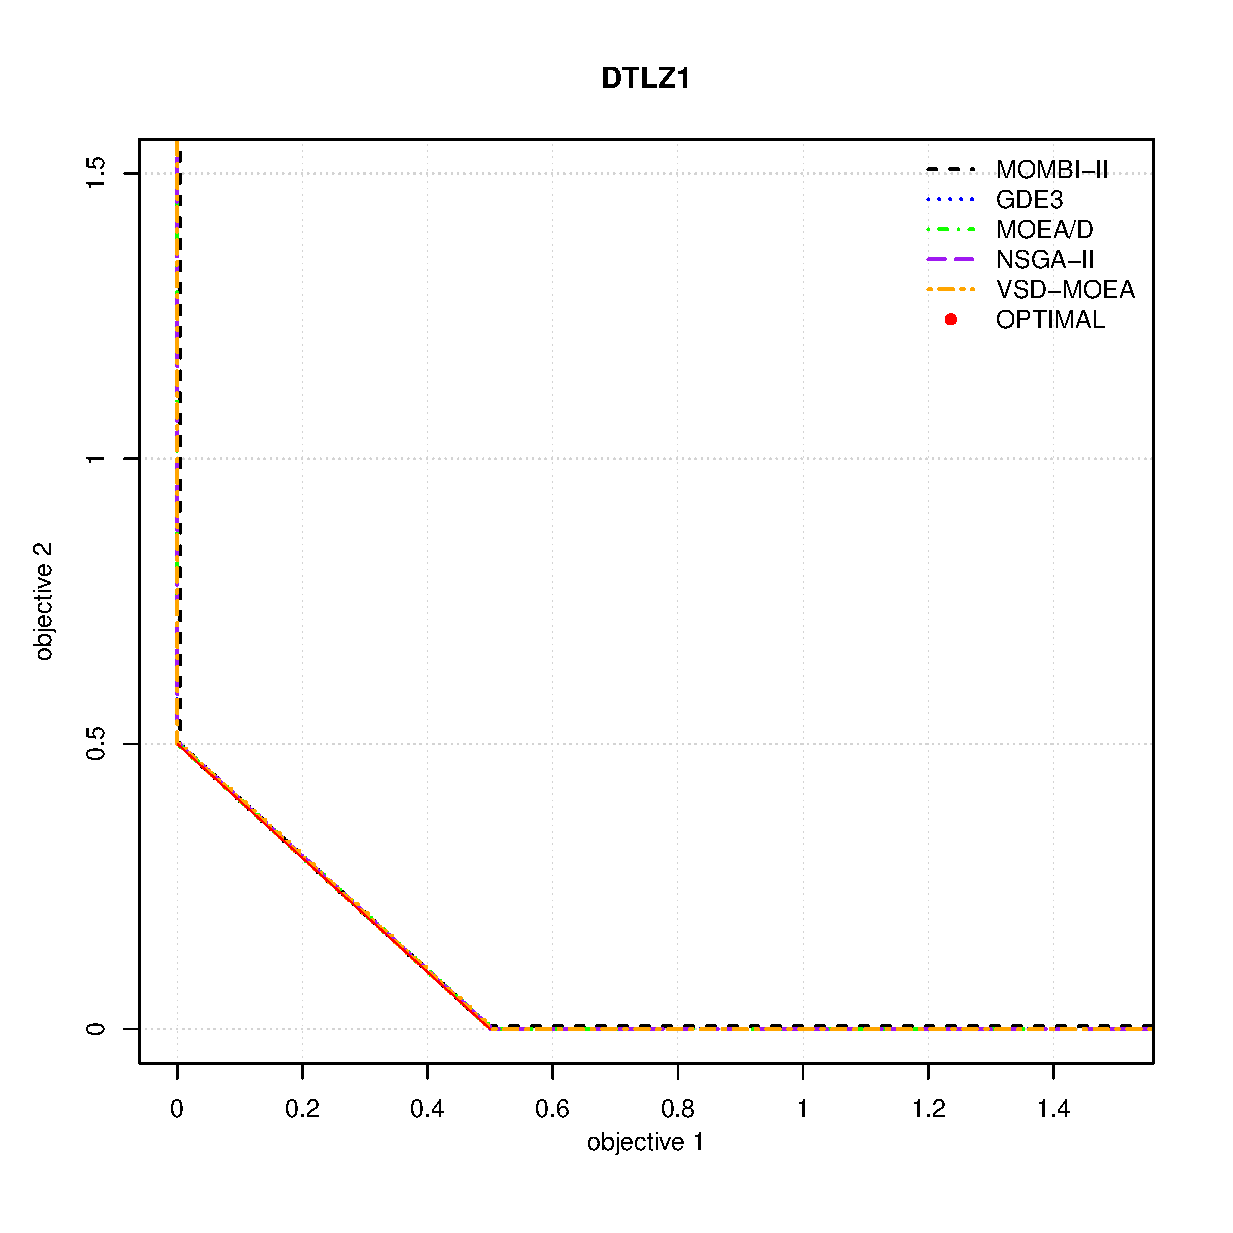
\includegraphics[width=0.33\textwidth]{Figures_Chapter7/Results_Chapter3/DTLZ1.eps} &
  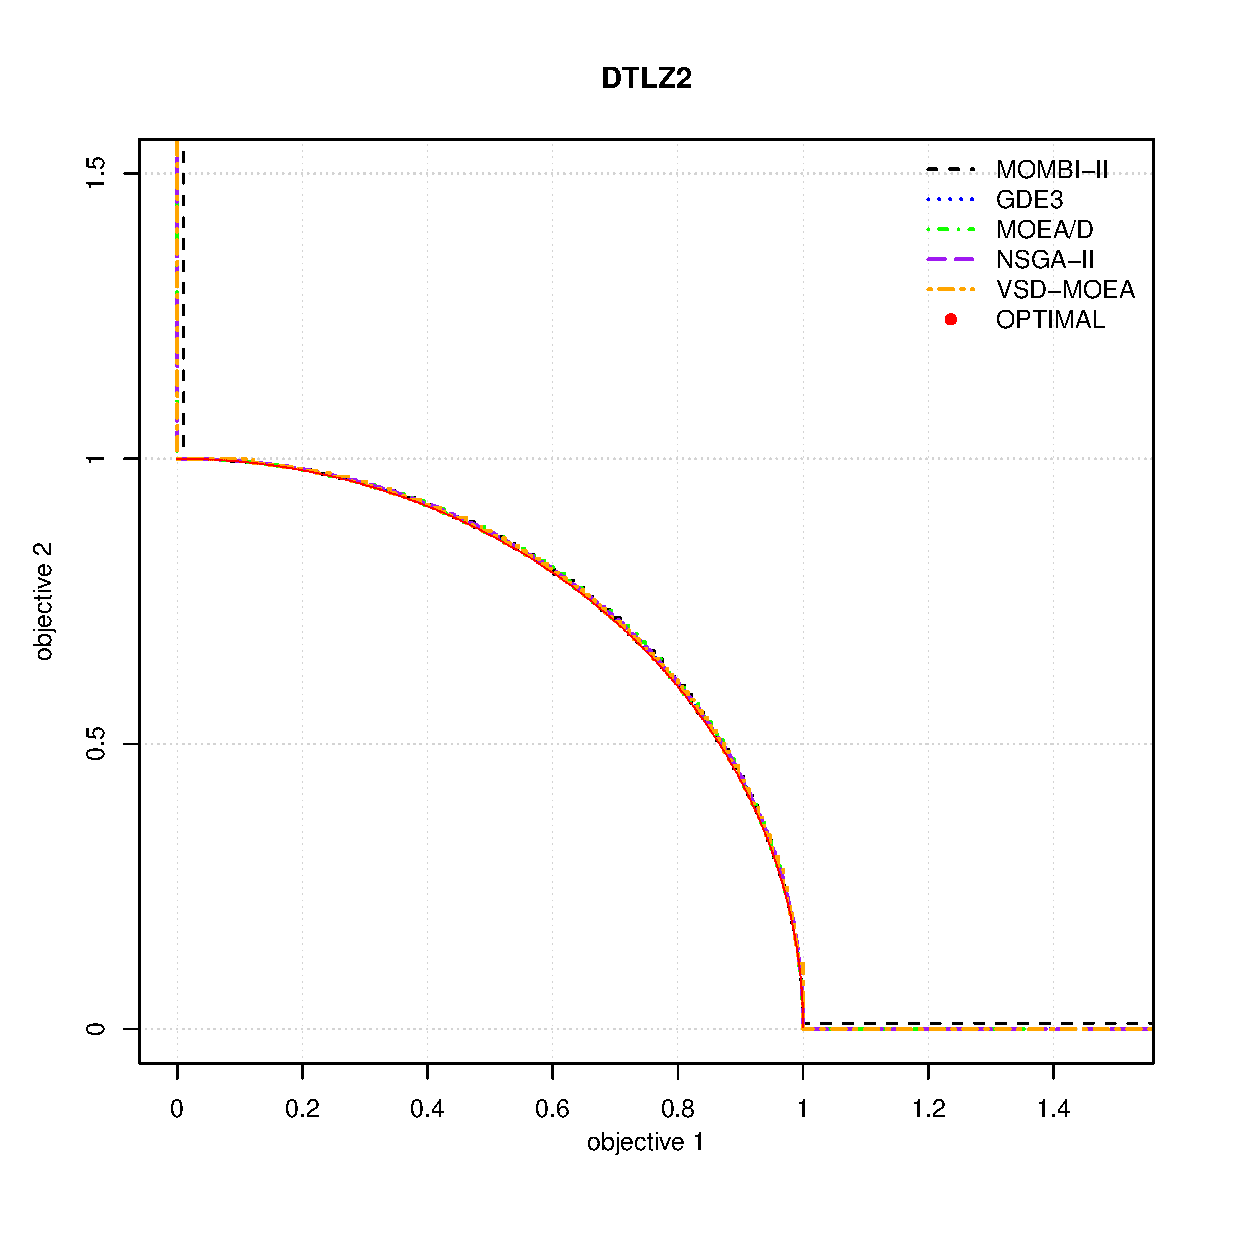
\includegraphics[width=0.33\textwidth]{Figures_Chapter7/Results_Chapter3/DTLZ2.eps} &
  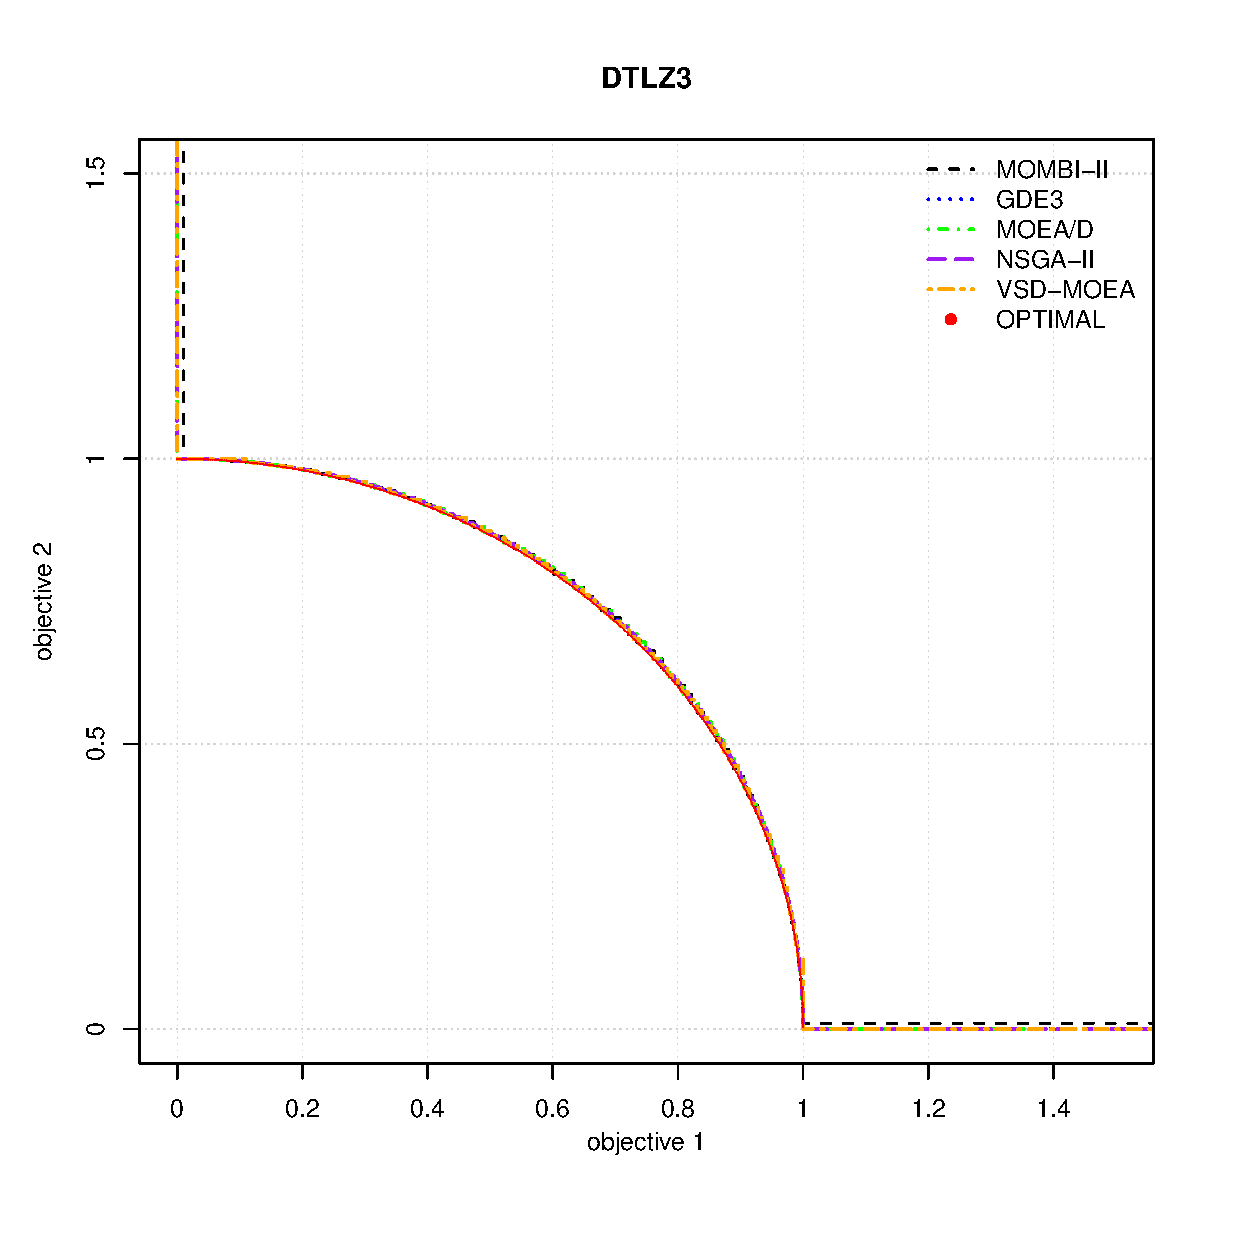
\includegraphics[width=0.33\textwidth]{Figures_Chapter7/Results_Chapter3/DTLZ3.eps} \\
  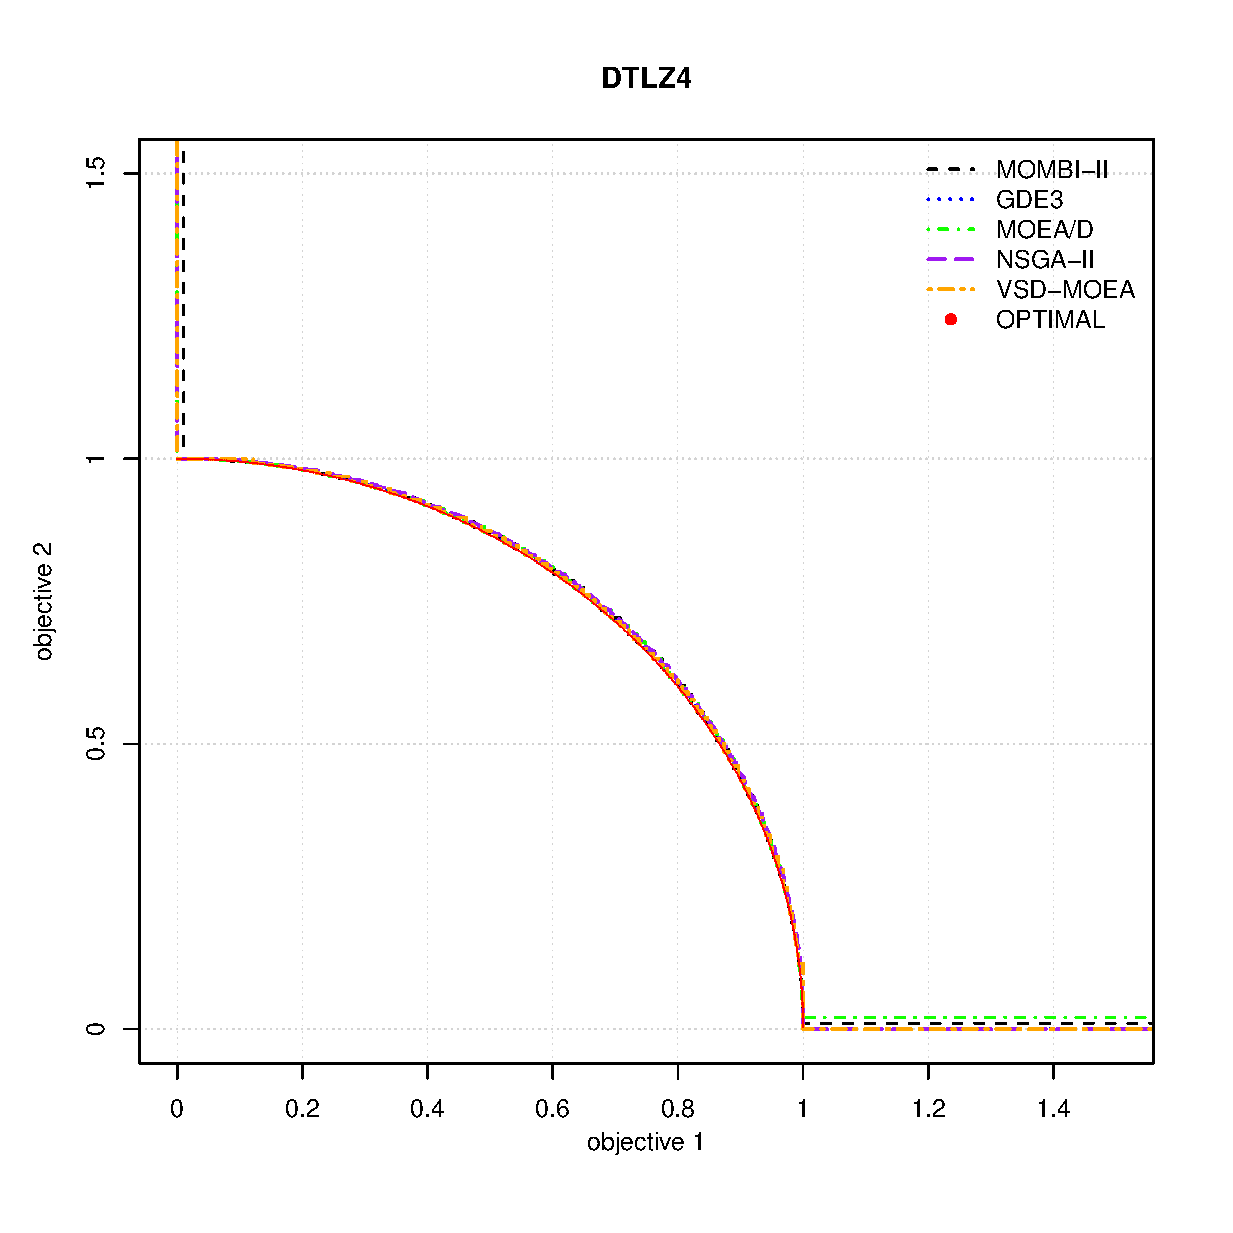
\includegraphics[width=0.33\textwidth]{Figures_Chapter7/Results_Chapter3/DTLZ4.eps} &
  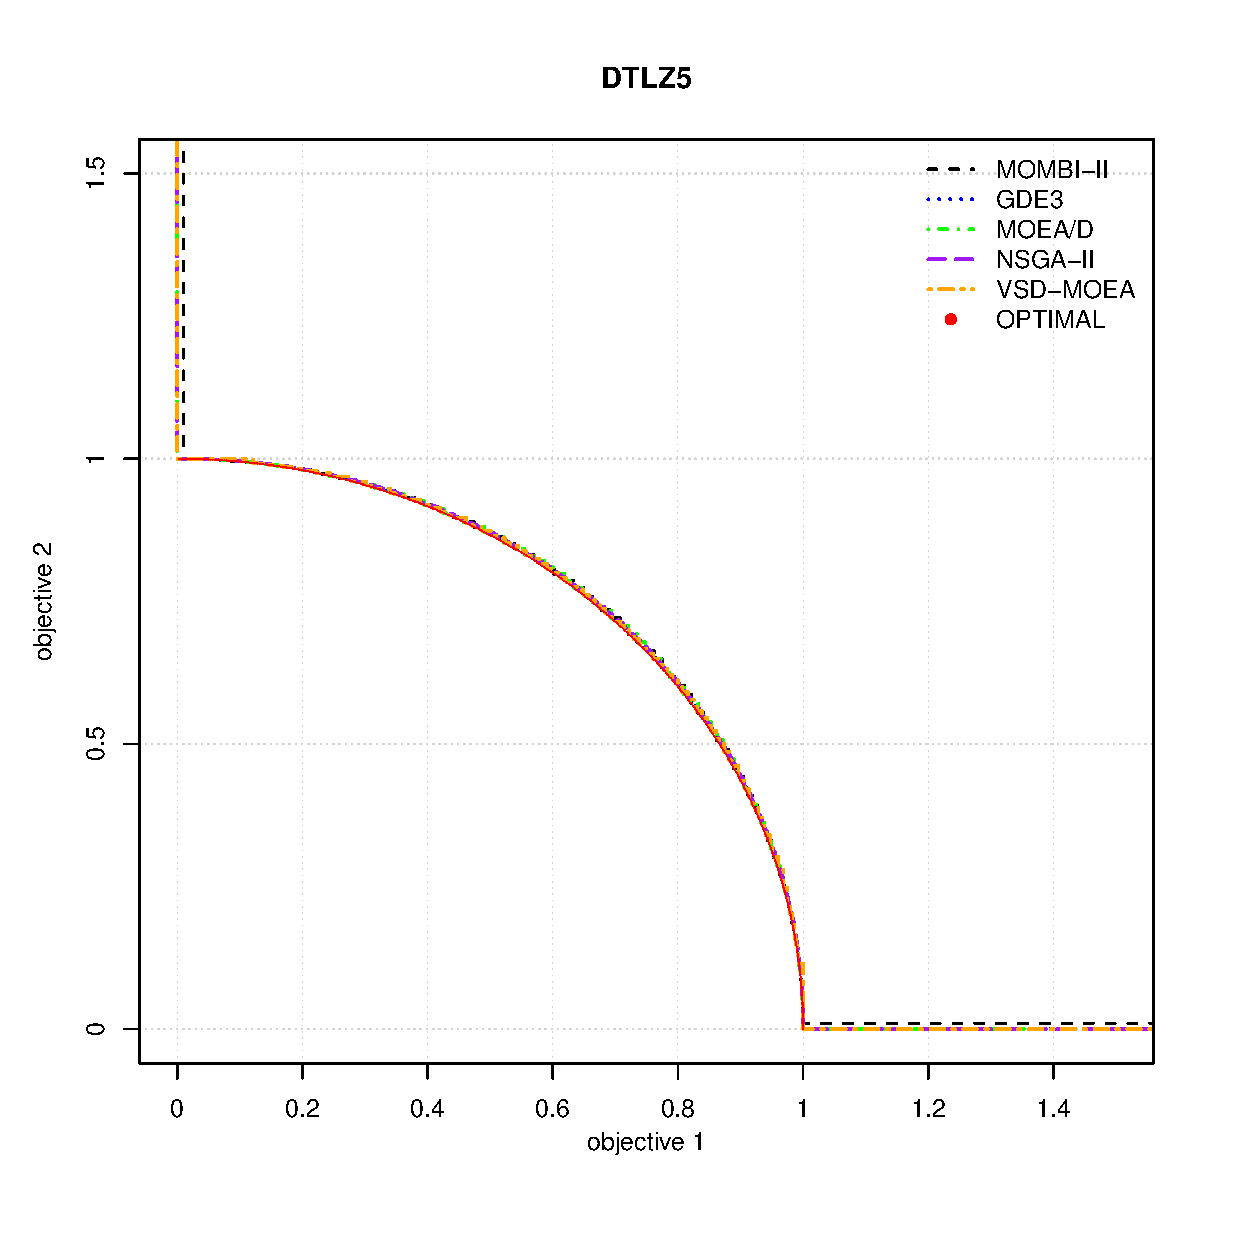
\includegraphics[width=0.33\textwidth]{Figures_Chapter7/Results_Chapter3/DTLZ5.eps} &
  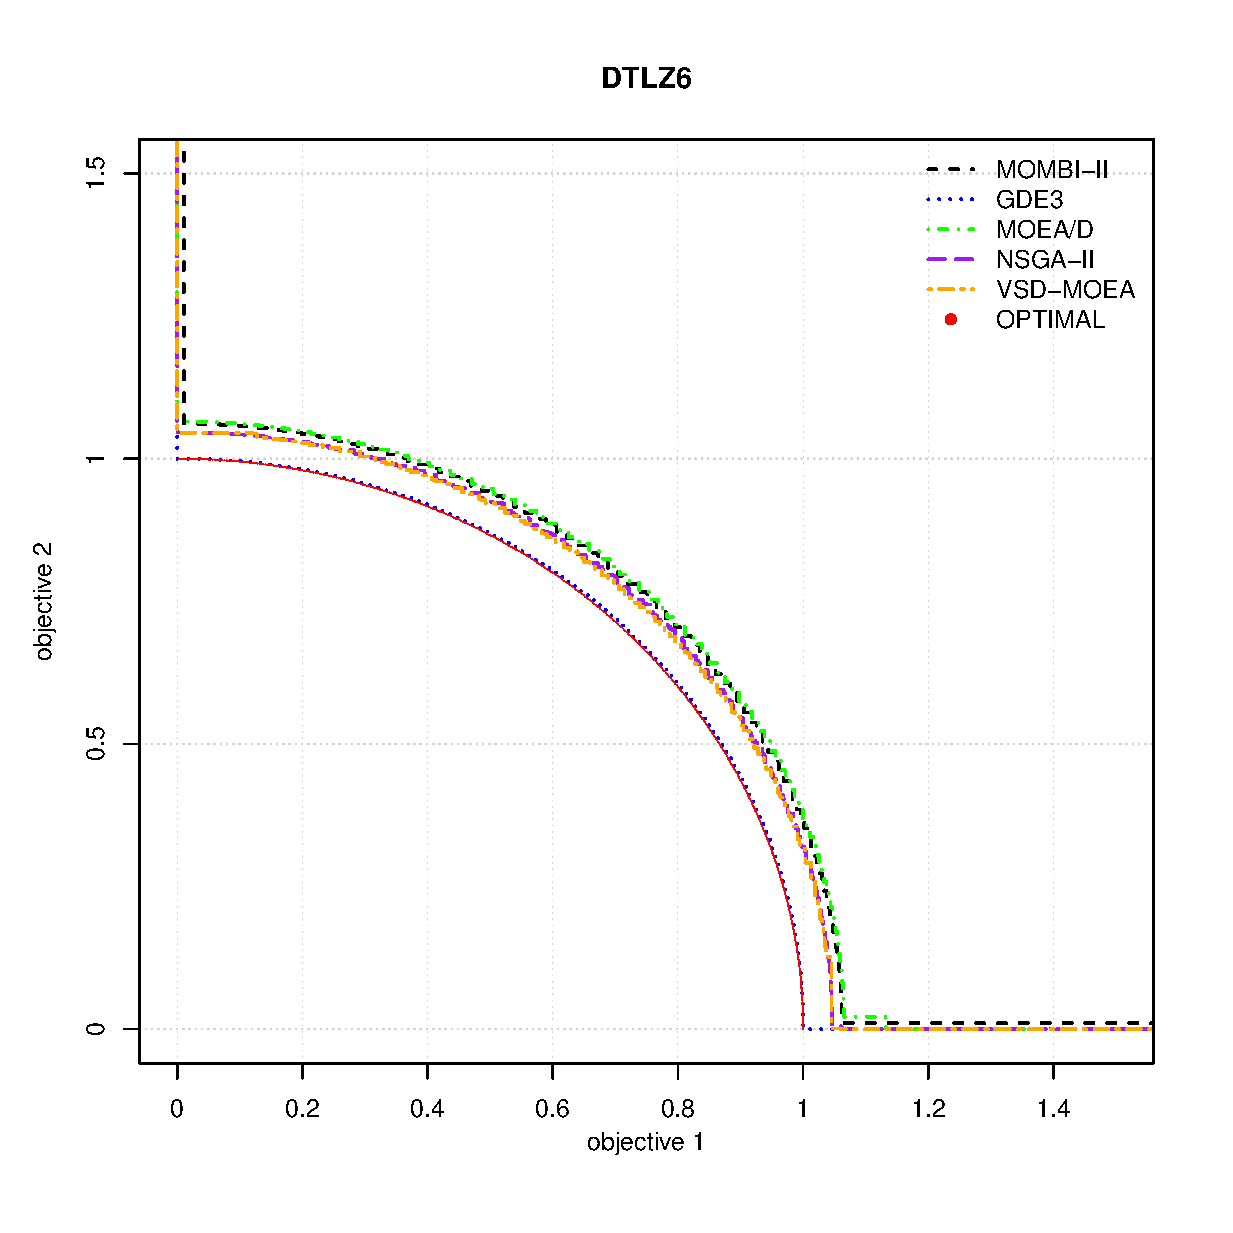
\includegraphics[width=0.33\textwidth]{Figures_Chapter7/Results_Chapter3/DTLZ6.eps} \\
  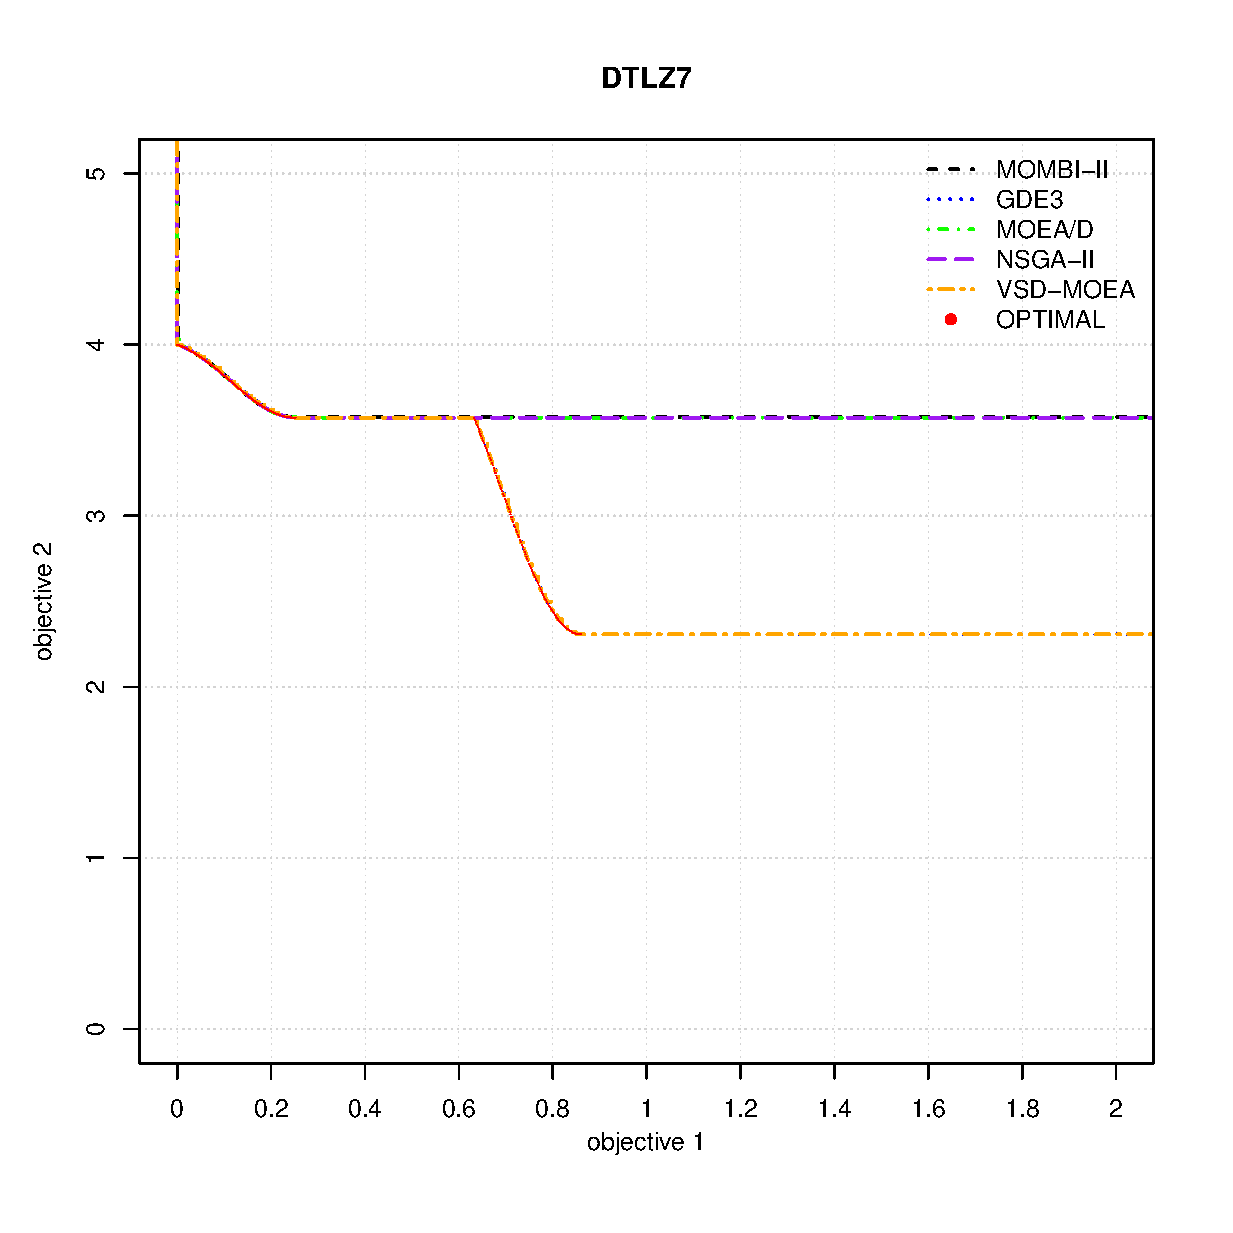
\includegraphics[width=0.33\textwidth]{Figures_Chapter7/Results_Chapter3/DTLZ7.eps}
  \end{tabular}
\end{figure*}
 
 \begin{figure*}[h]
\centering
\caption{superficies de cubrimiento logradas al 50\%}%Attainment Figures\_Chapter7 Achieved}
\begin{tabular}{ccc}
  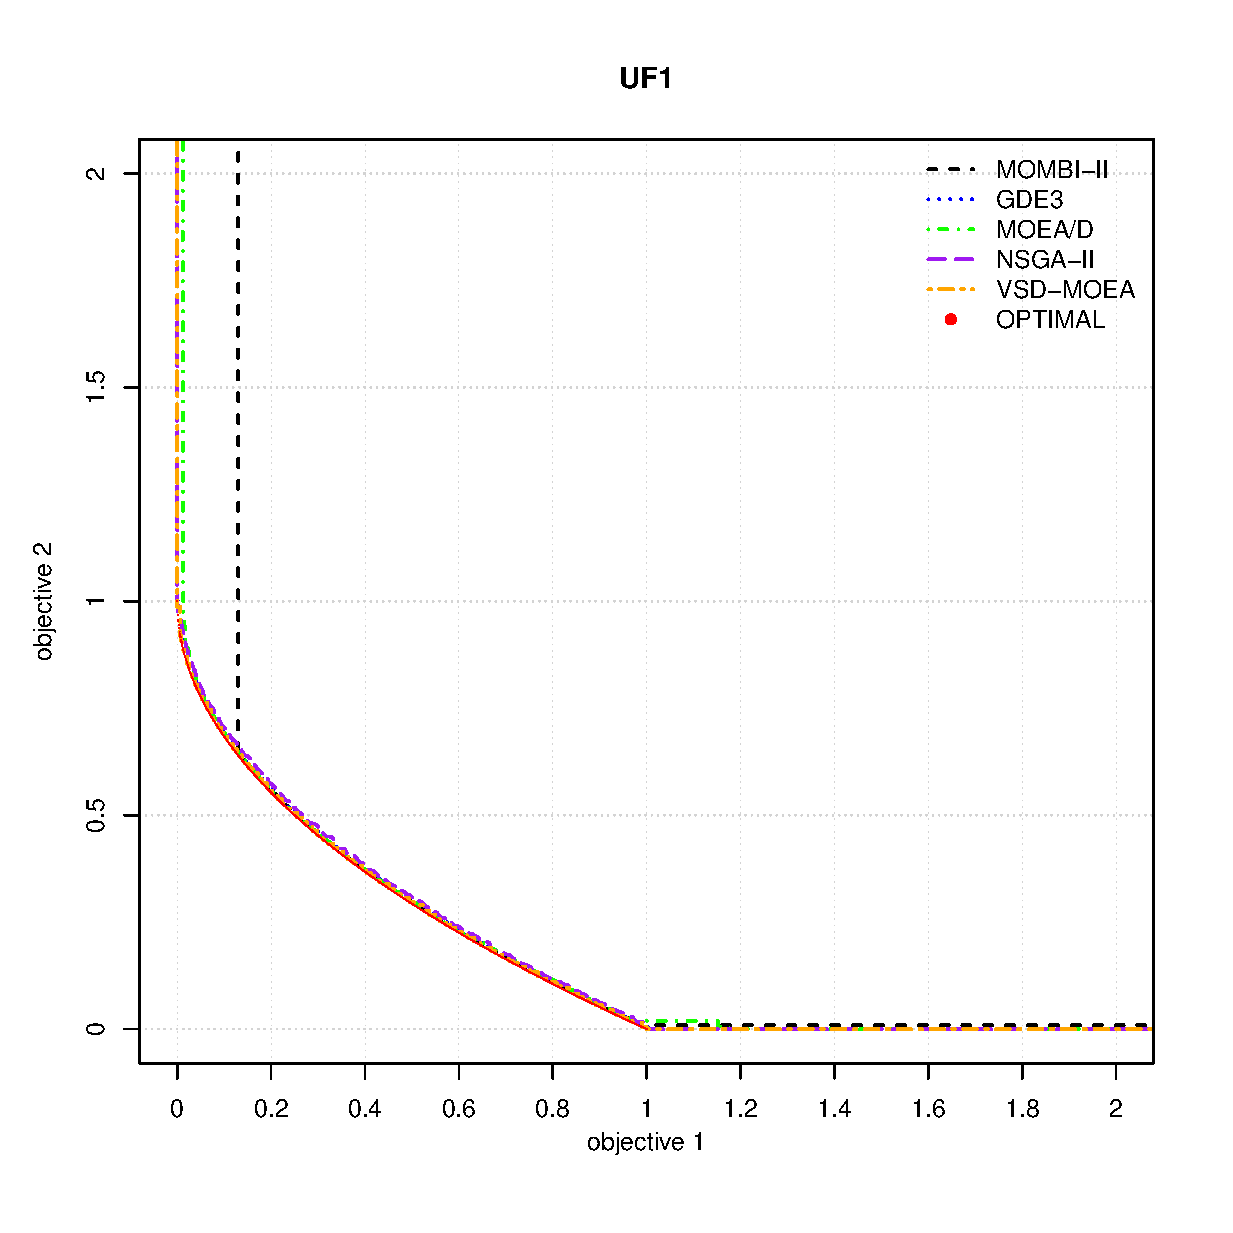
\includegraphics[width=0.33\textwidth]{Figures_Chapter7/Results_Chapter3/UF1.eps} &
  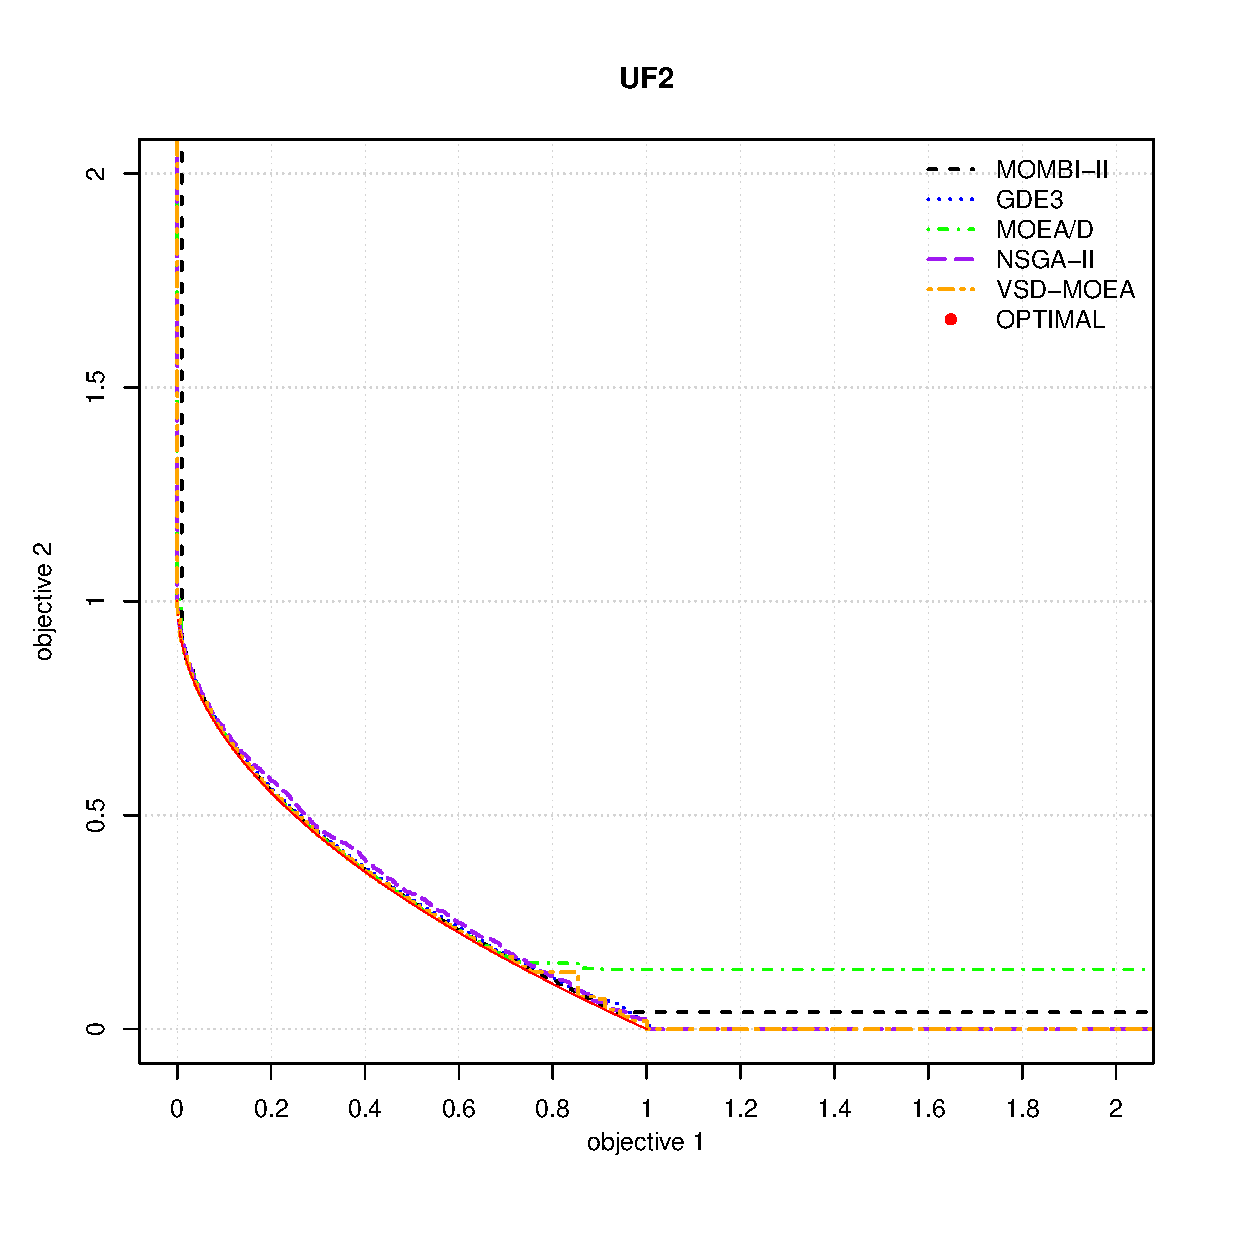
\includegraphics[width=0.33\textwidth]{Figures_Chapter7/Results_Chapter3/UF2.eps} &
  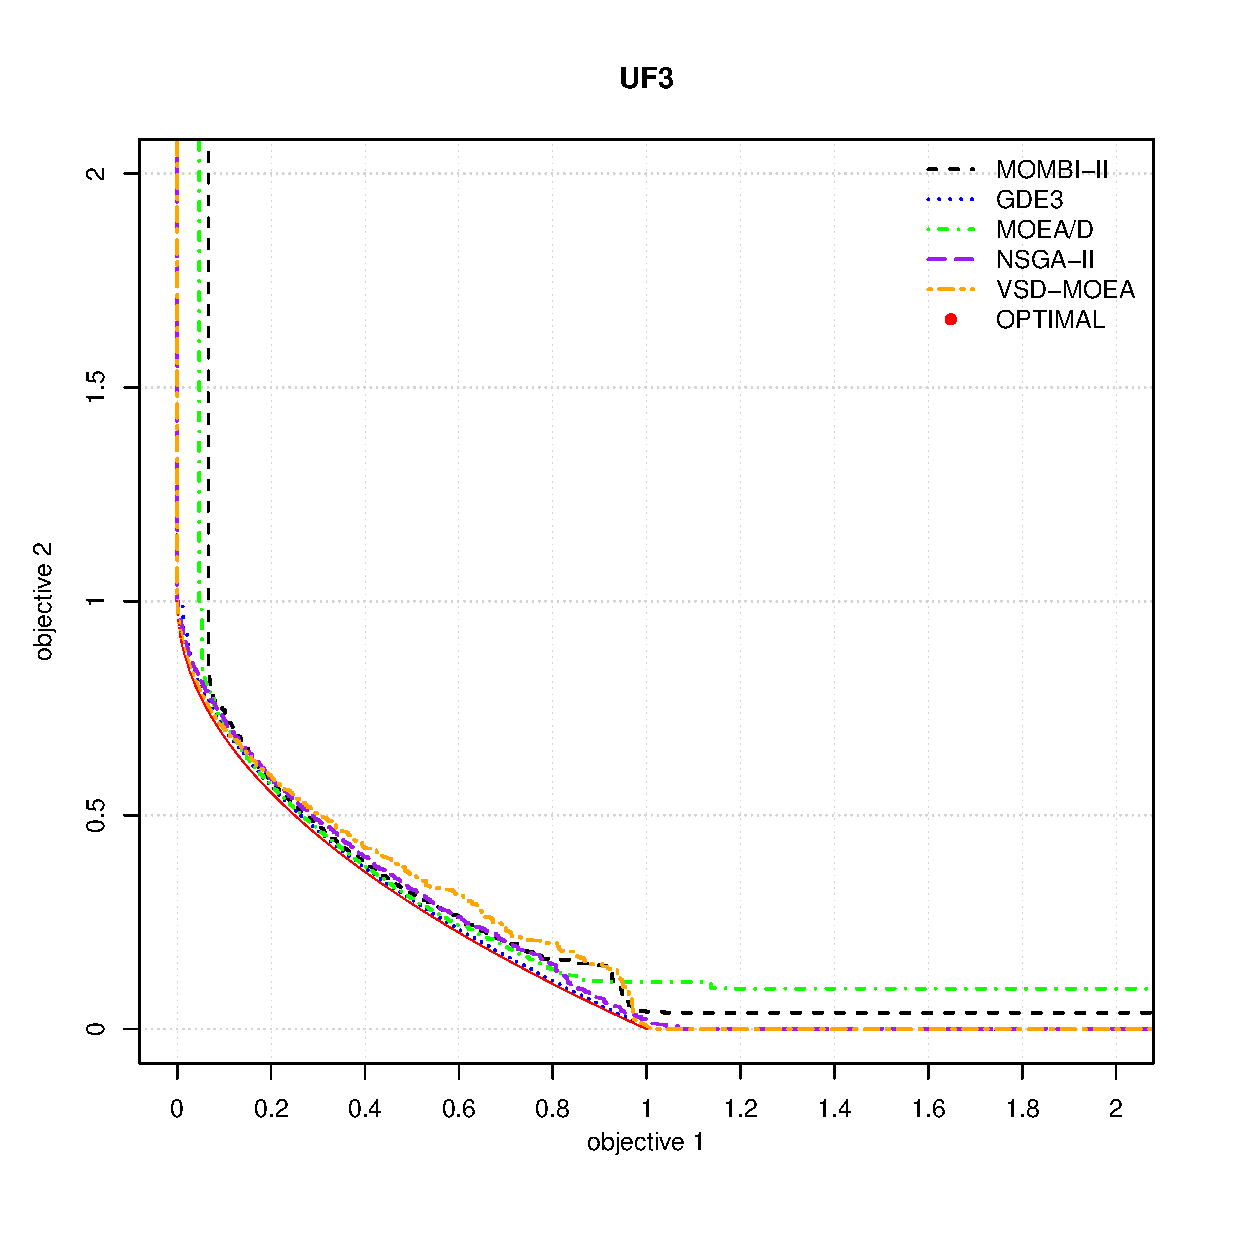
\includegraphics[width=0.33\textwidth]{Figures_Chapter7/Results_Chapter3/UF3.eps} 
\\  
  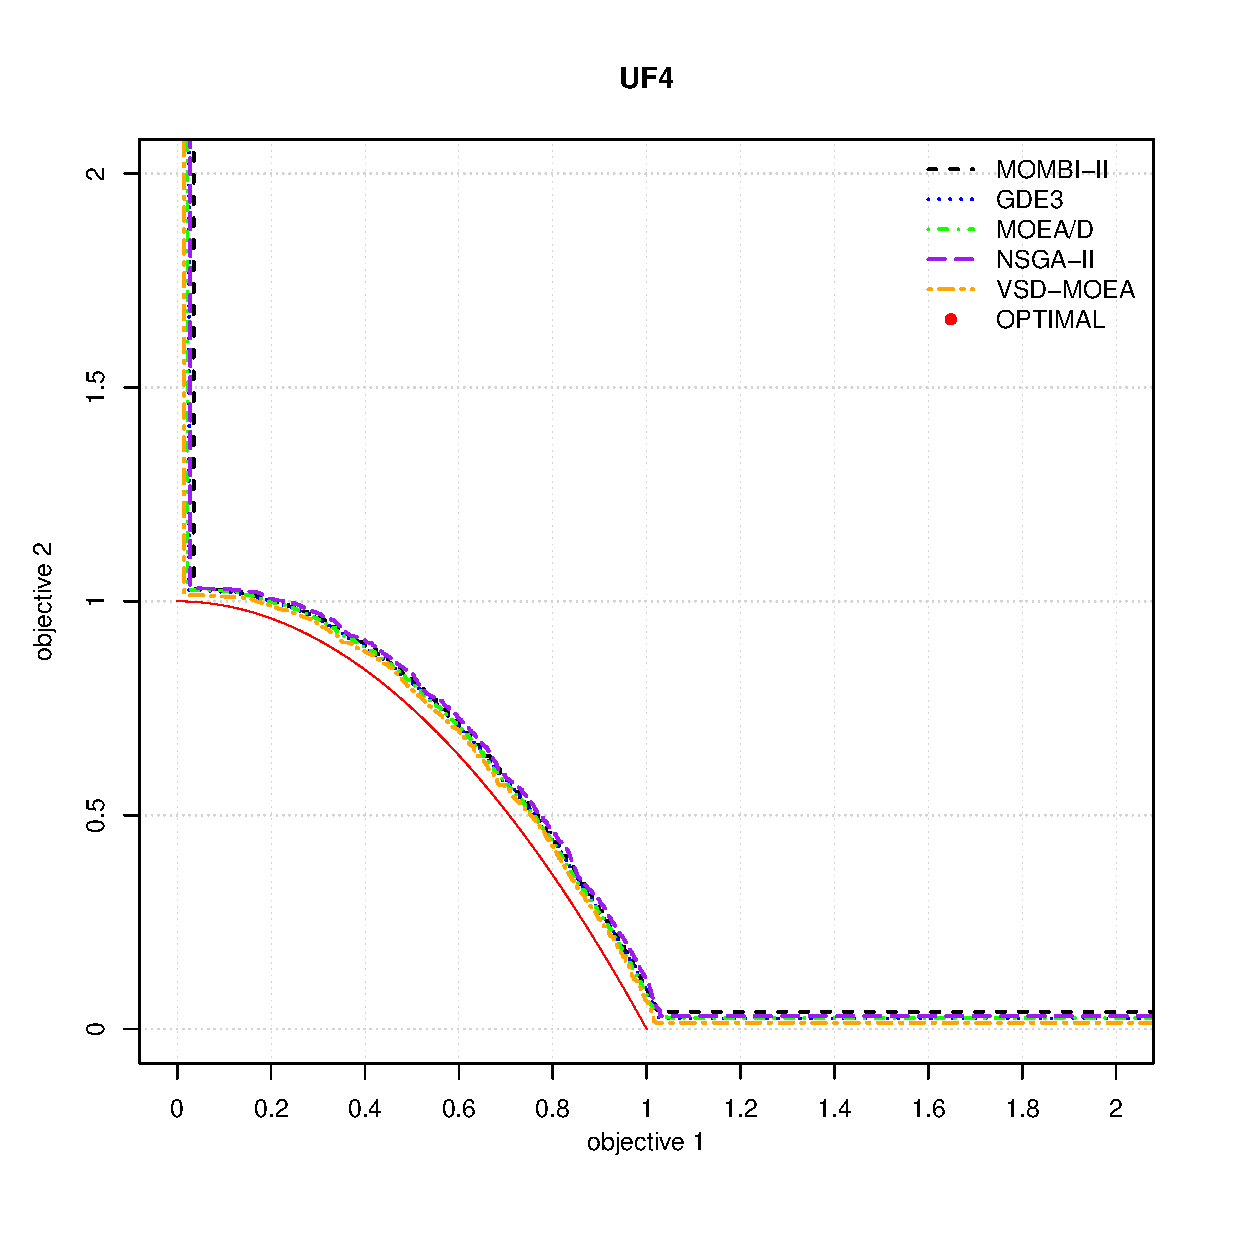
\includegraphics[width=0.33\textwidth]{Figures_Chapter7/Results_Chapter3/UF4.eps} &
  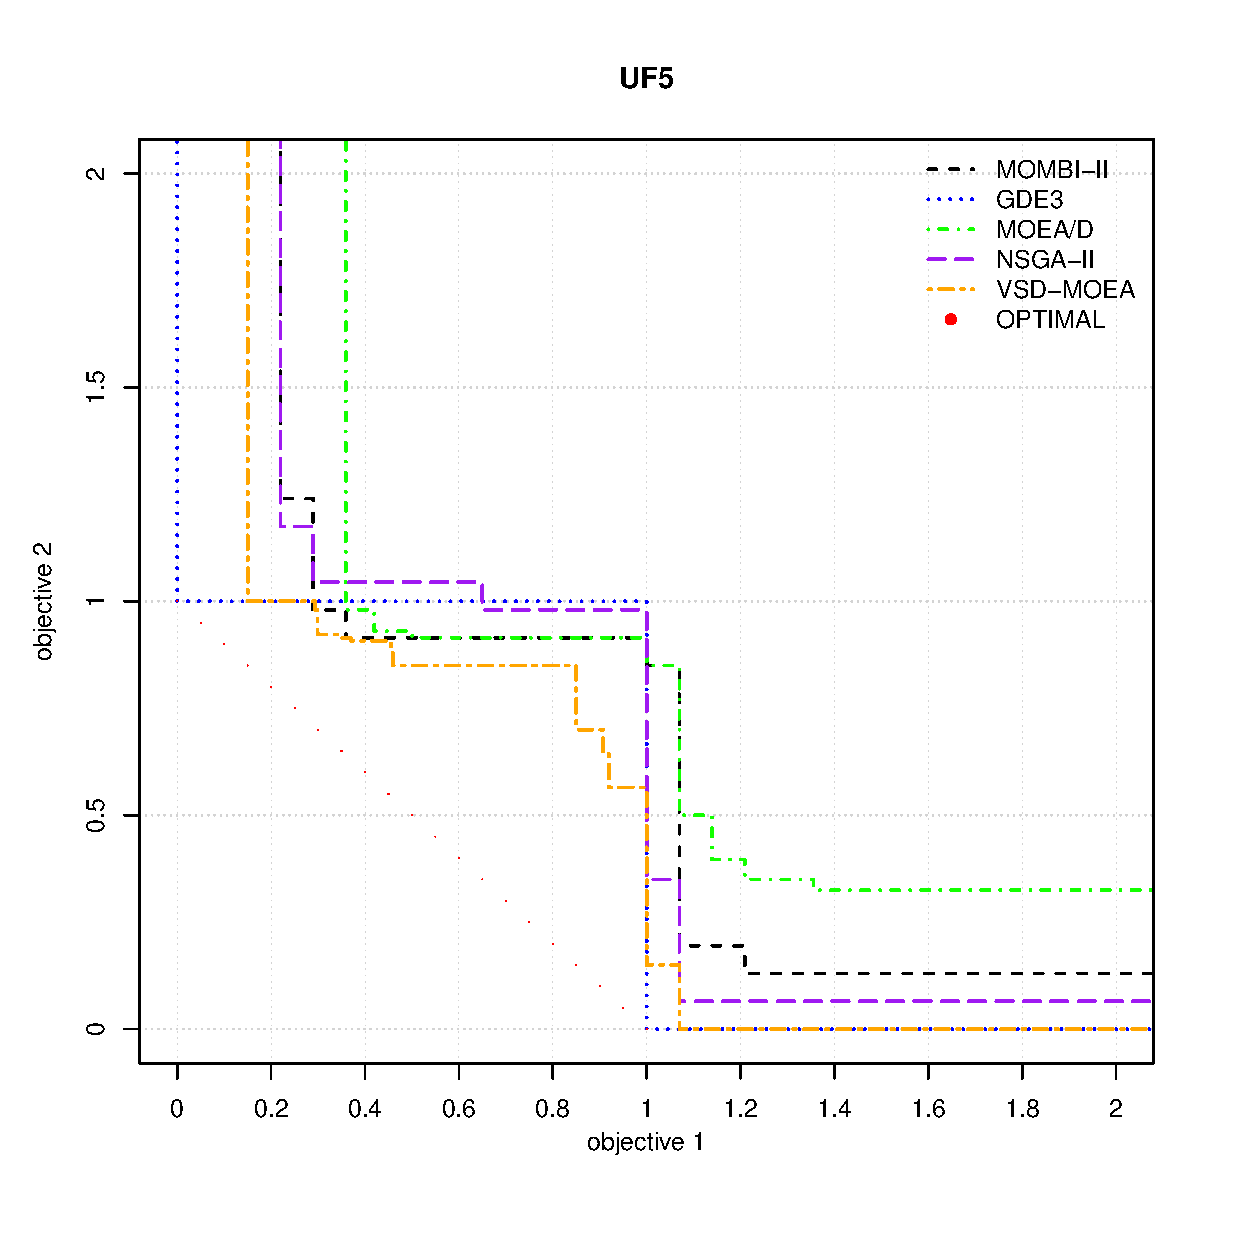
\includegraphics[width=0.33\textwidth]{Figures_Chapter7/Results_Chapter3/UF5.eps} &
  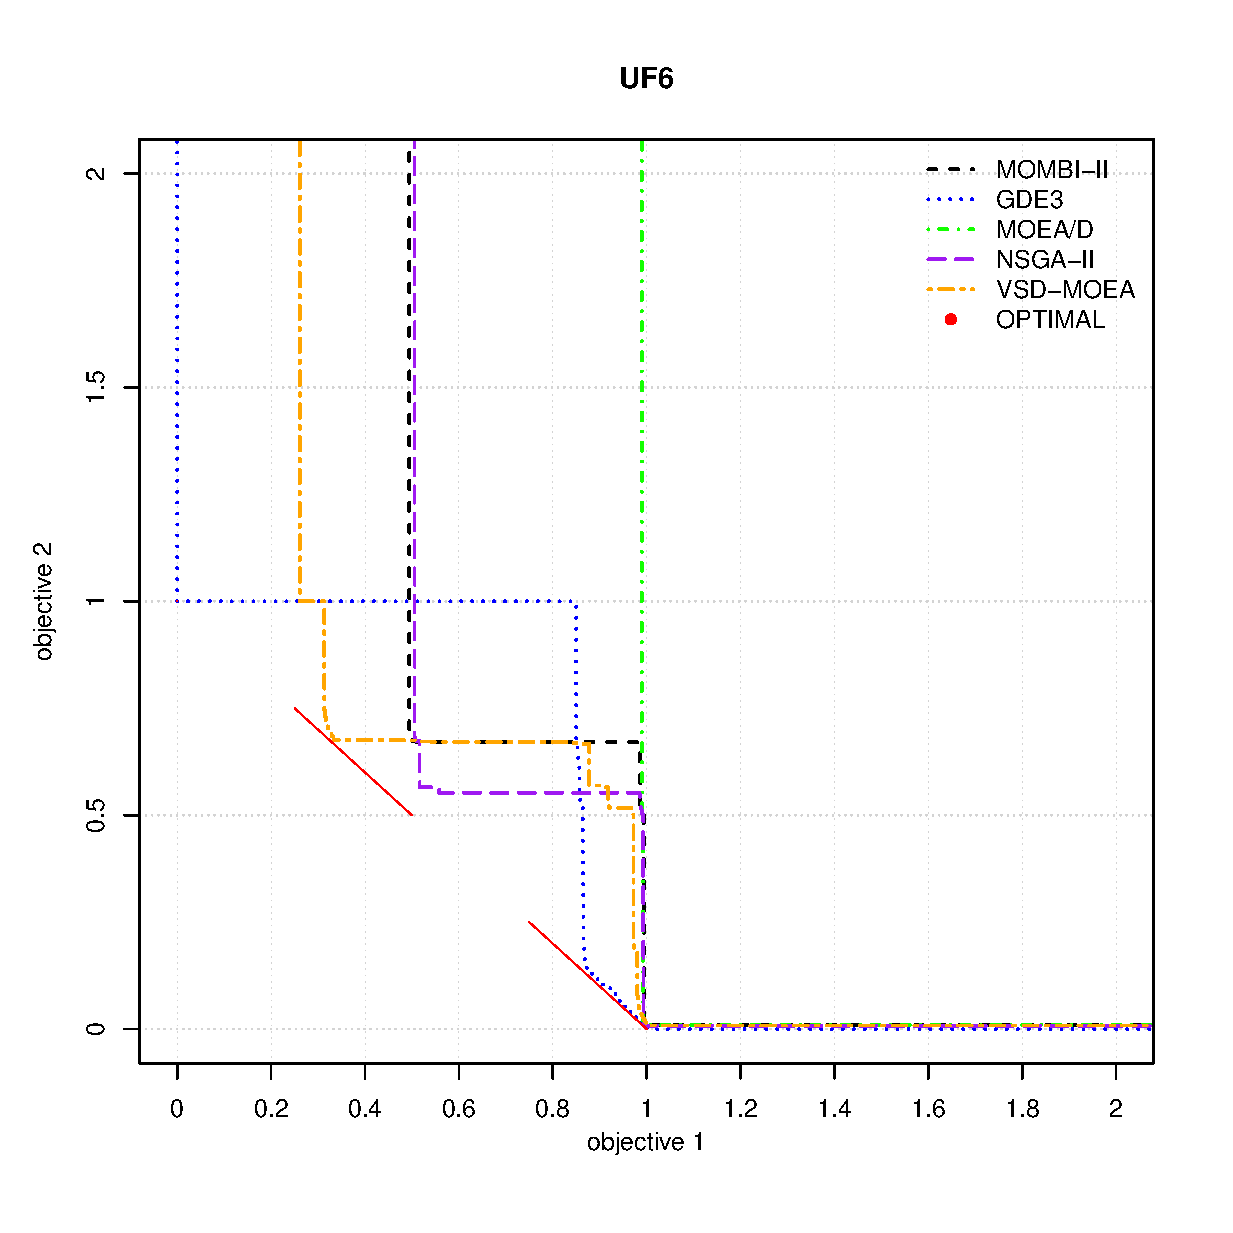
\includegraphics[width=0.33\textwidth]{Figures_Chapter7/Results_Chapter3/UF6.eps} 
\\
  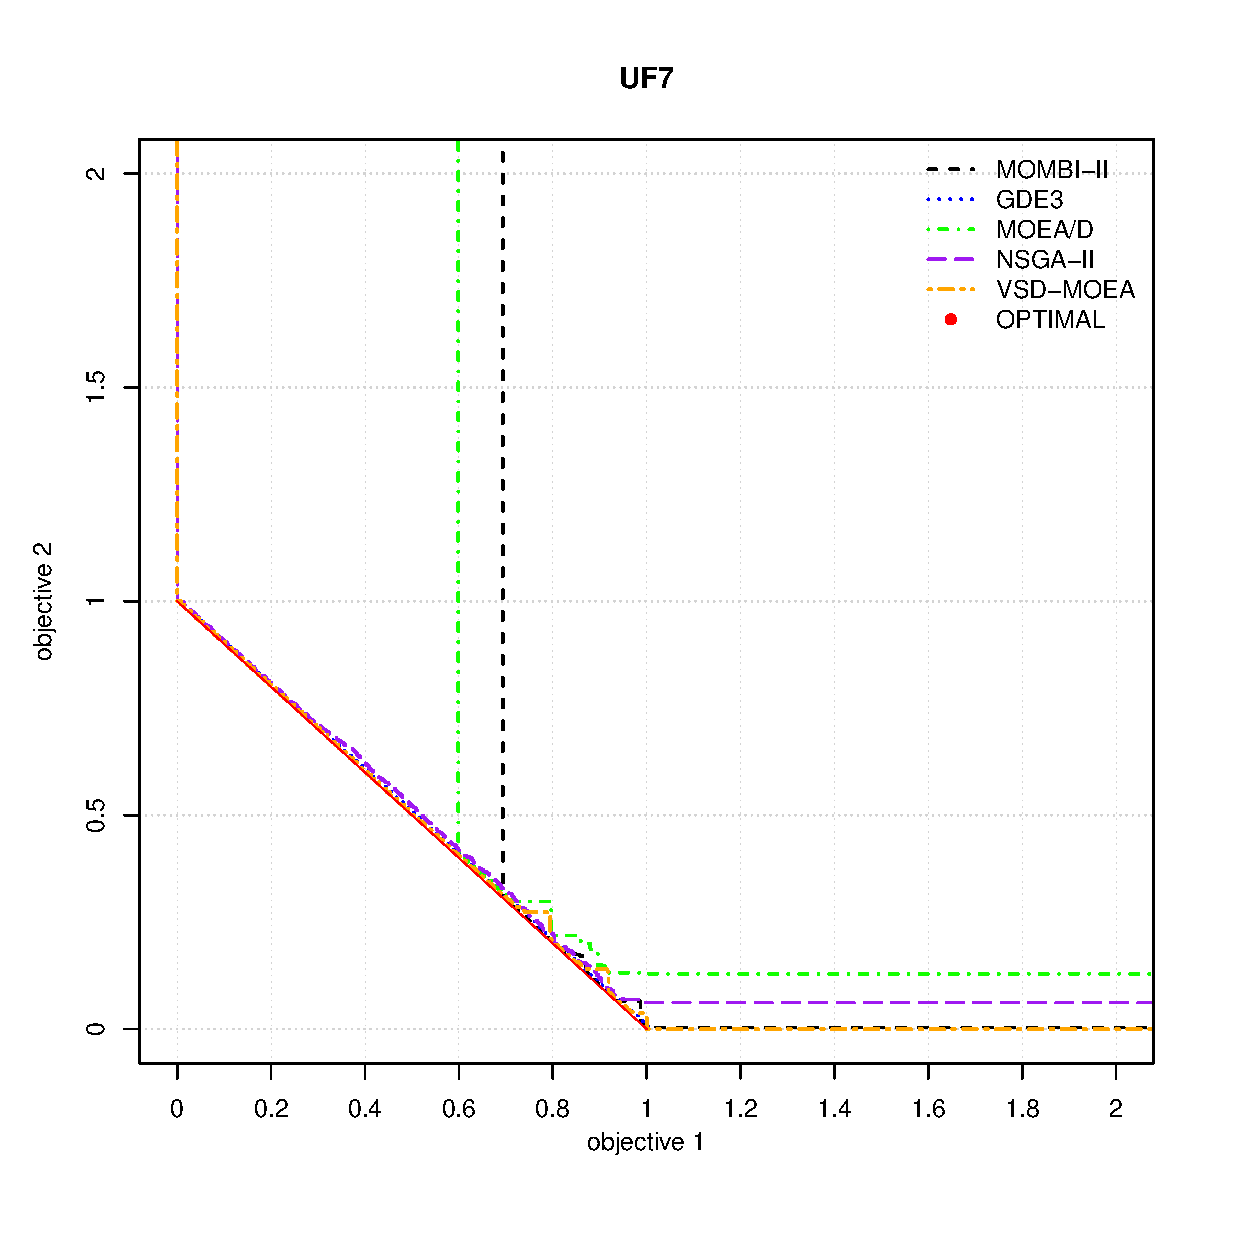
\includegraphics[width=0.33\textwidth]{Figures_Chapter7/Results_Chapter3/UF7.eps}
\end{tabular}
\end{figure*}  

\begin{figure*}[h]
\centering
\caption{superficies de cubrimiento logradas al 50\%}%Attainment Figures\_Chapter7 Achieved}
\begin{tabular}{ccc}
  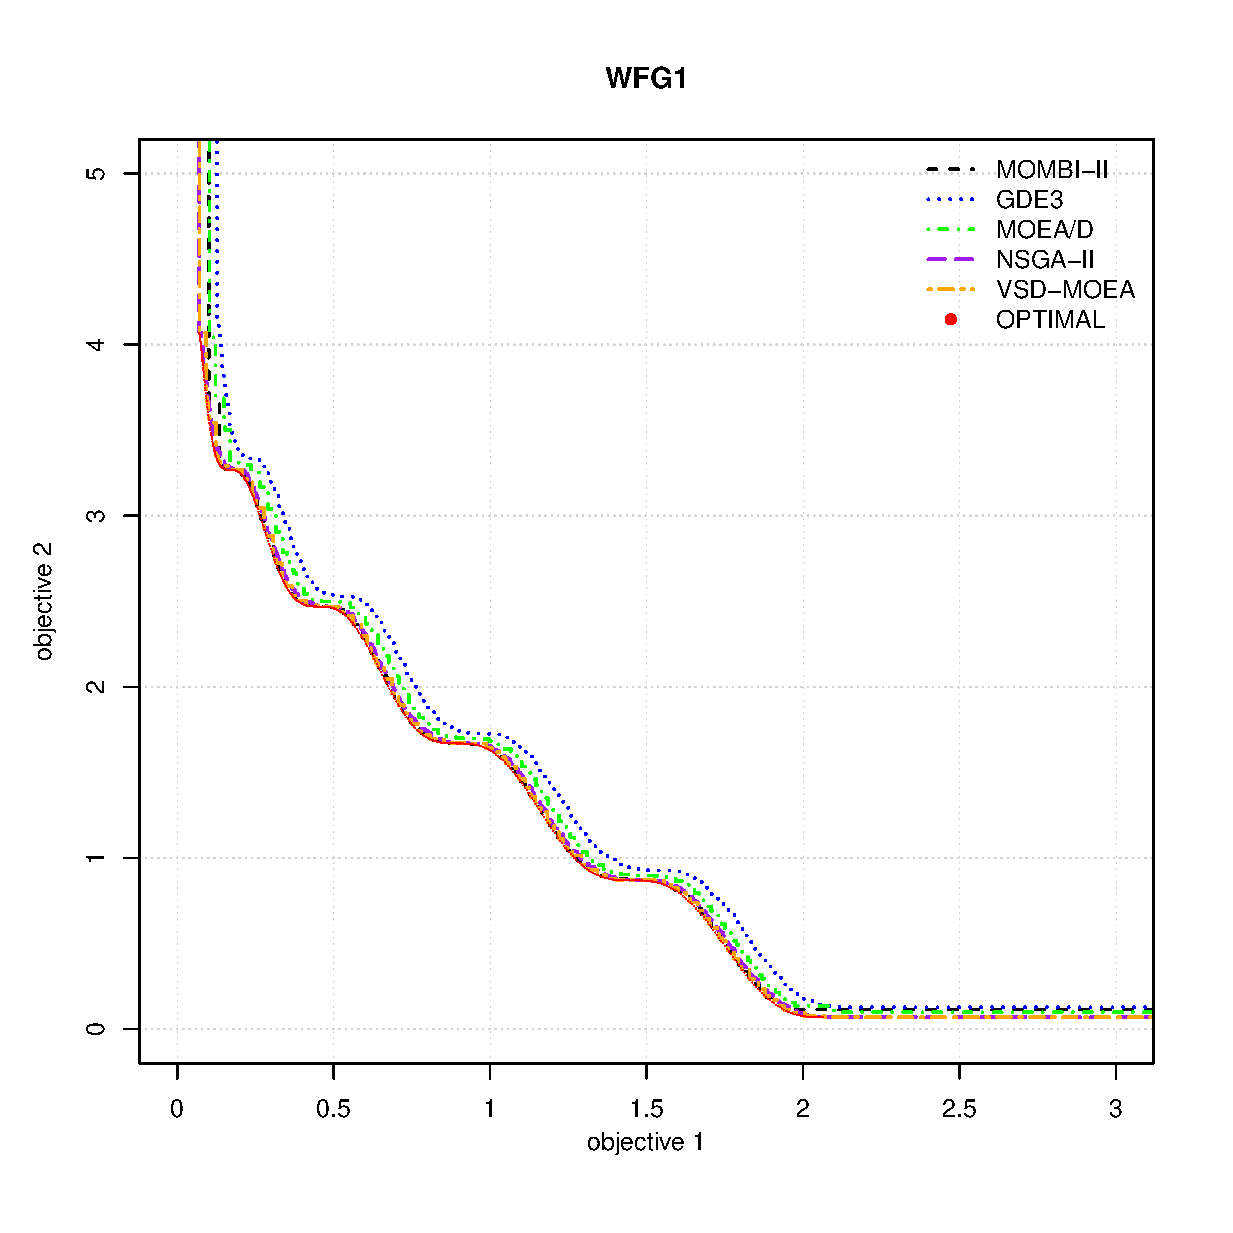
\includegraphics[width=0.33\textwidth]{Figures_Chapter7/Results_Chapter3/WFG1.eps} &
  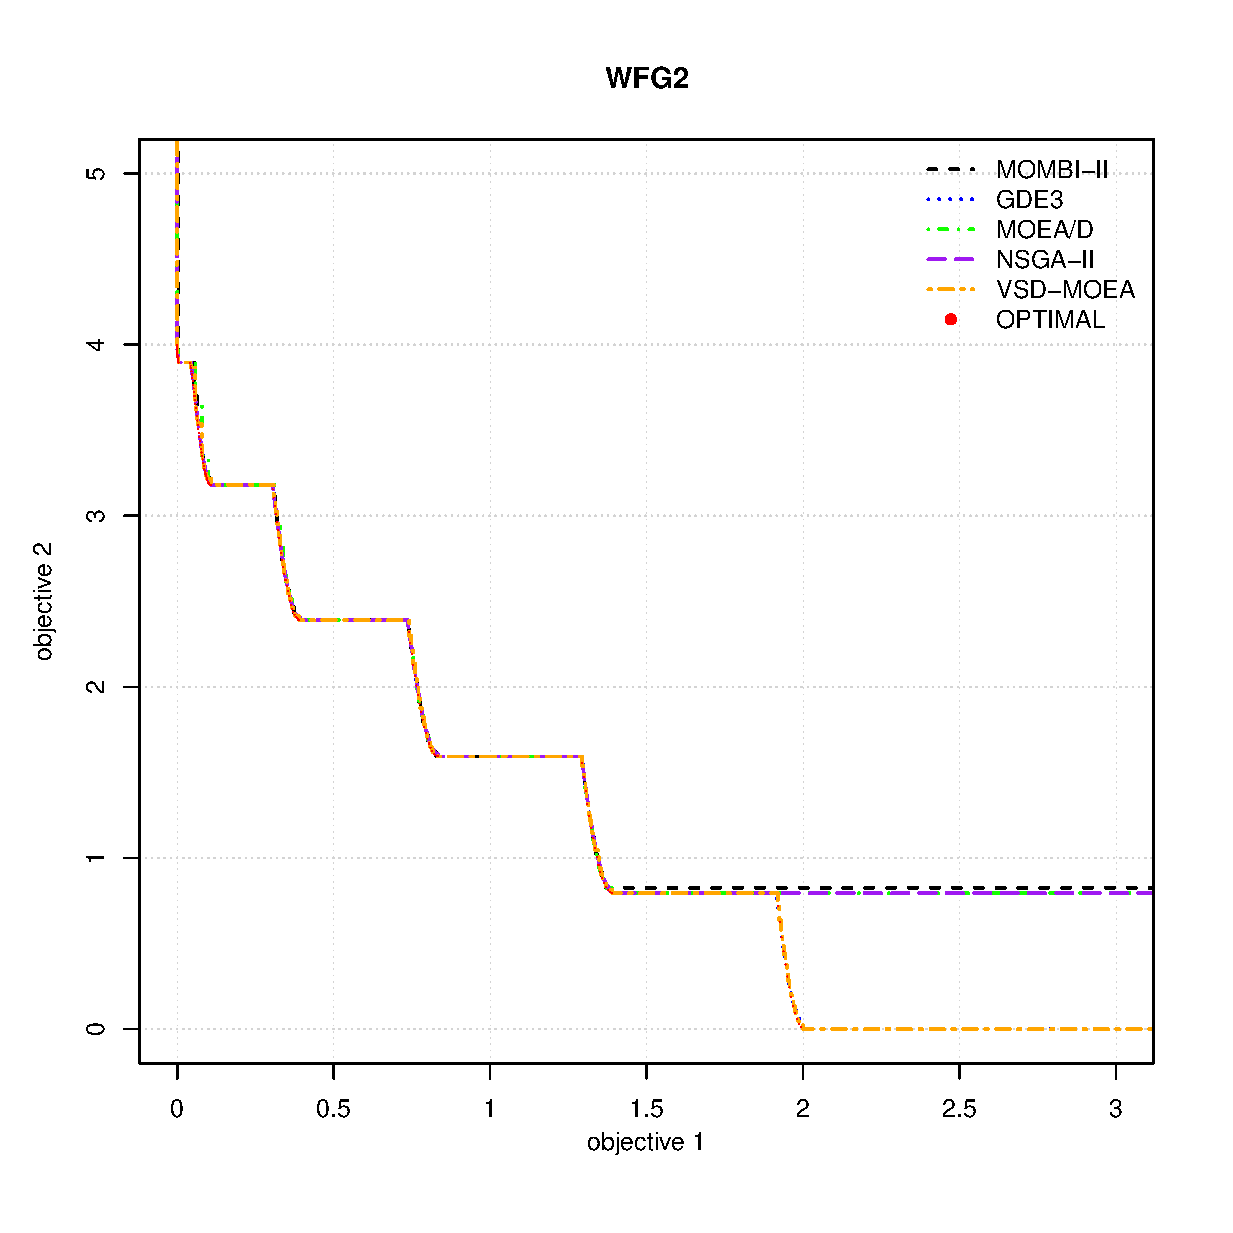
\includegraphics[width=0.33\textwidth]{Figures_Chapter7/Results_Chapter3/WFG2.eps} &
  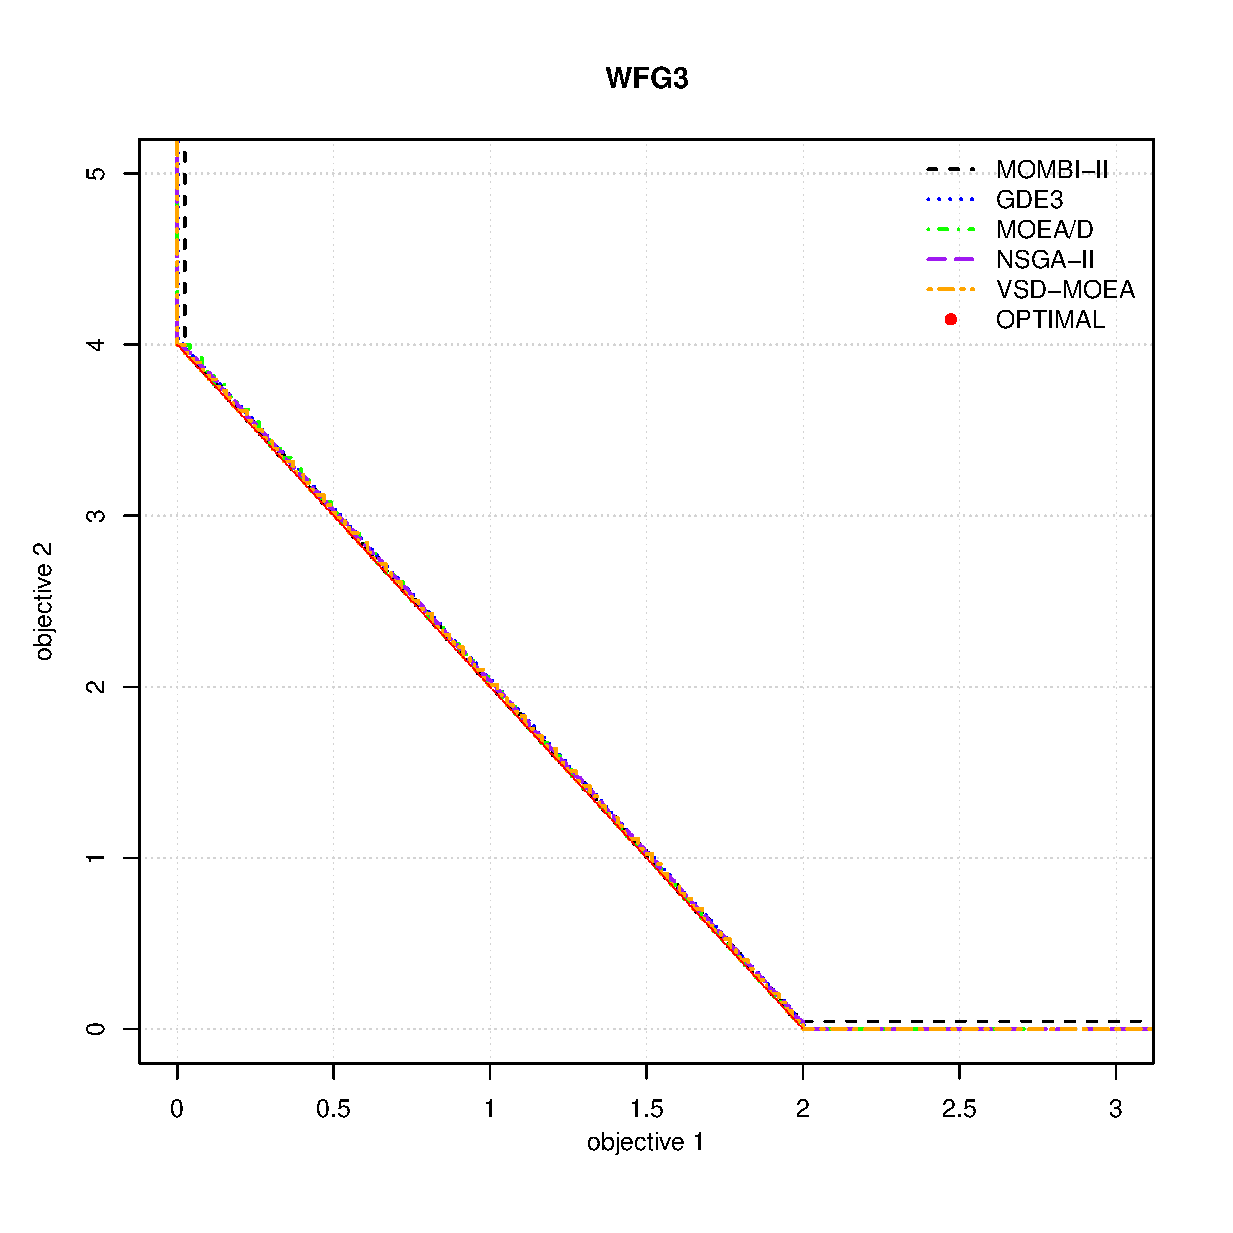
\includegraphics[width=0.33\textwidth]{Figures_Chapter7/Results_Chapter3/WFG3.eps} 
\\
  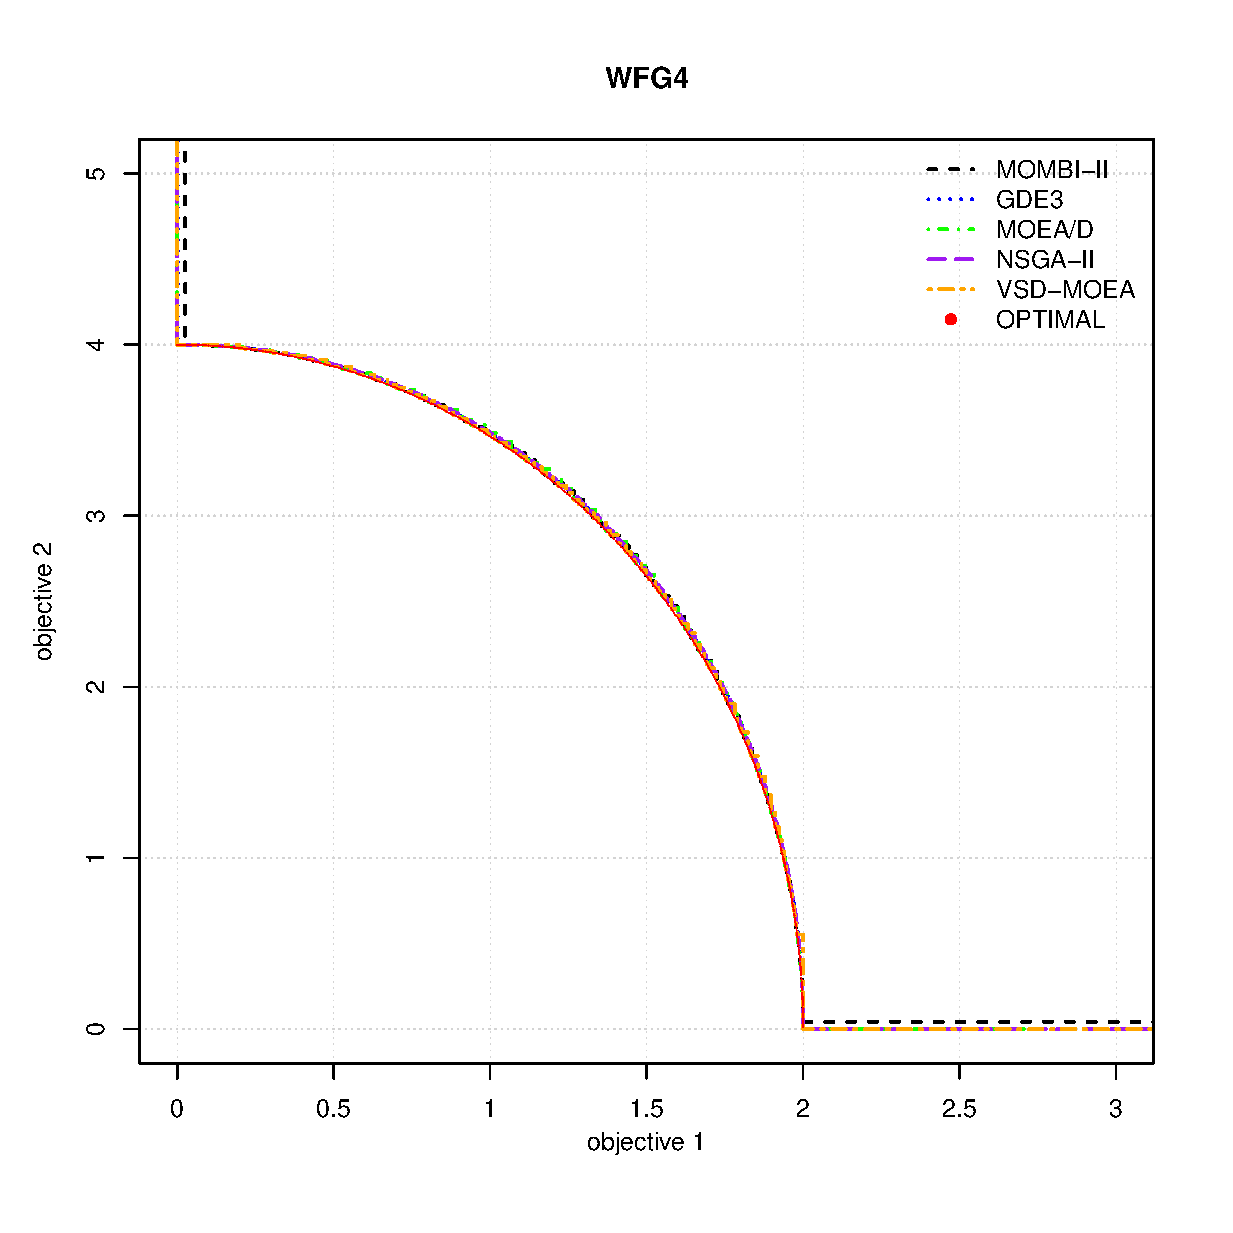
\includegraphics[width=0.33\textwidth]{Figures_Chapter7/Results_Chapter3/WFG4.eps} &
  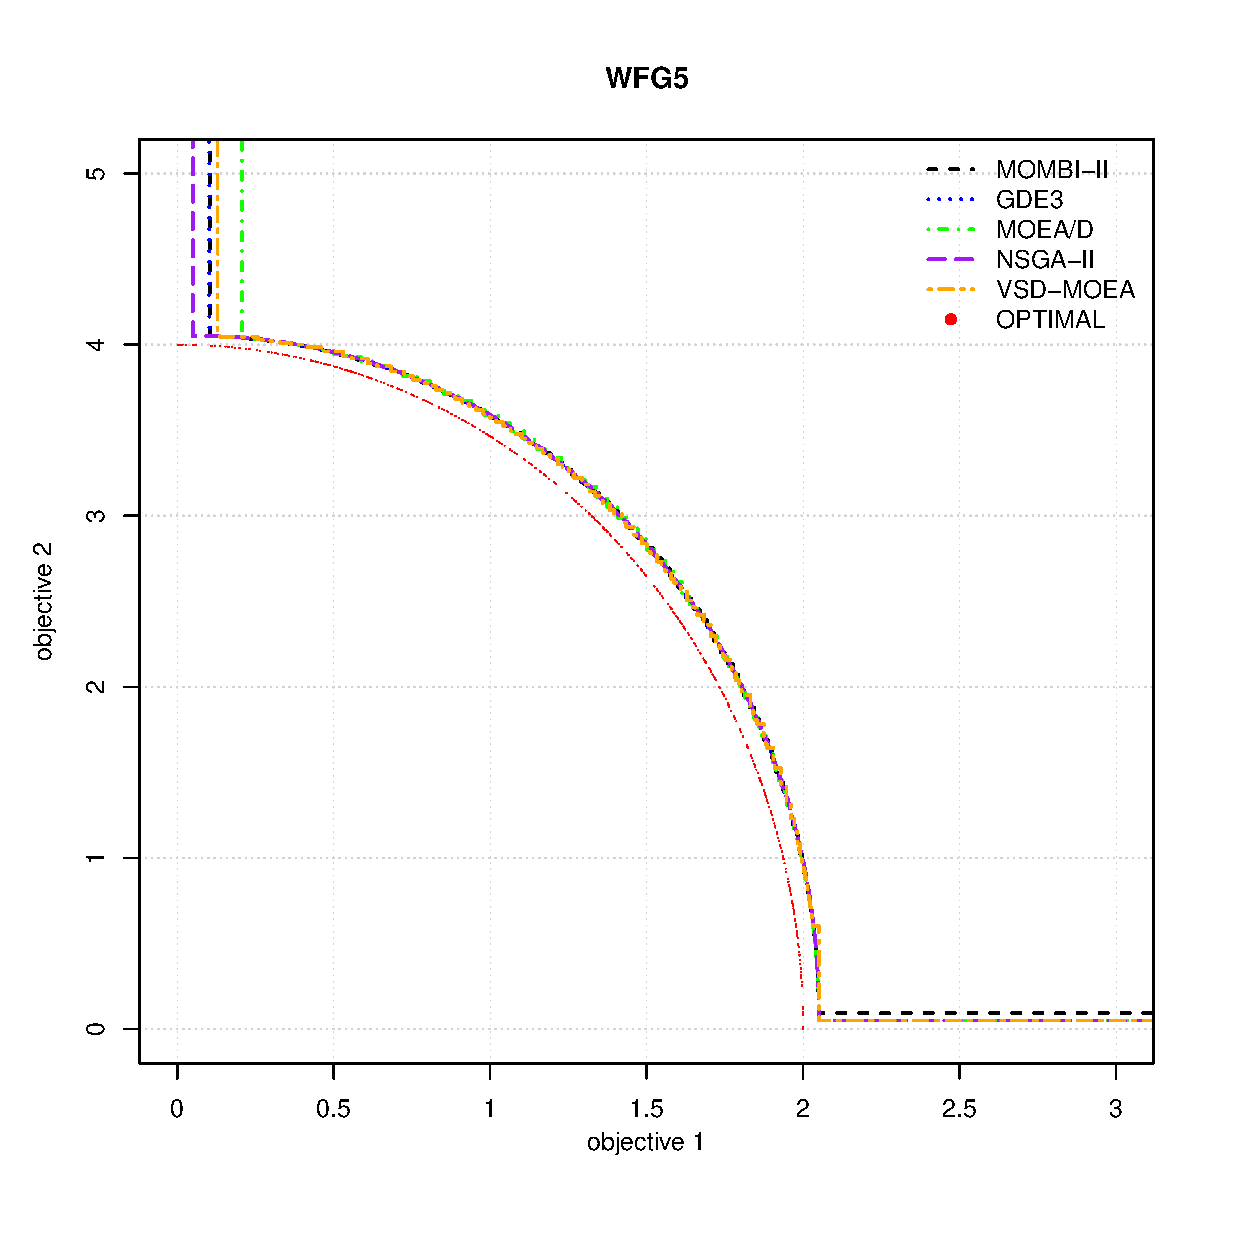
\includegraphics[width=0.33\textwidth]{Figures_Chapter7/Results_Chapter3/WFG5.eps} &
  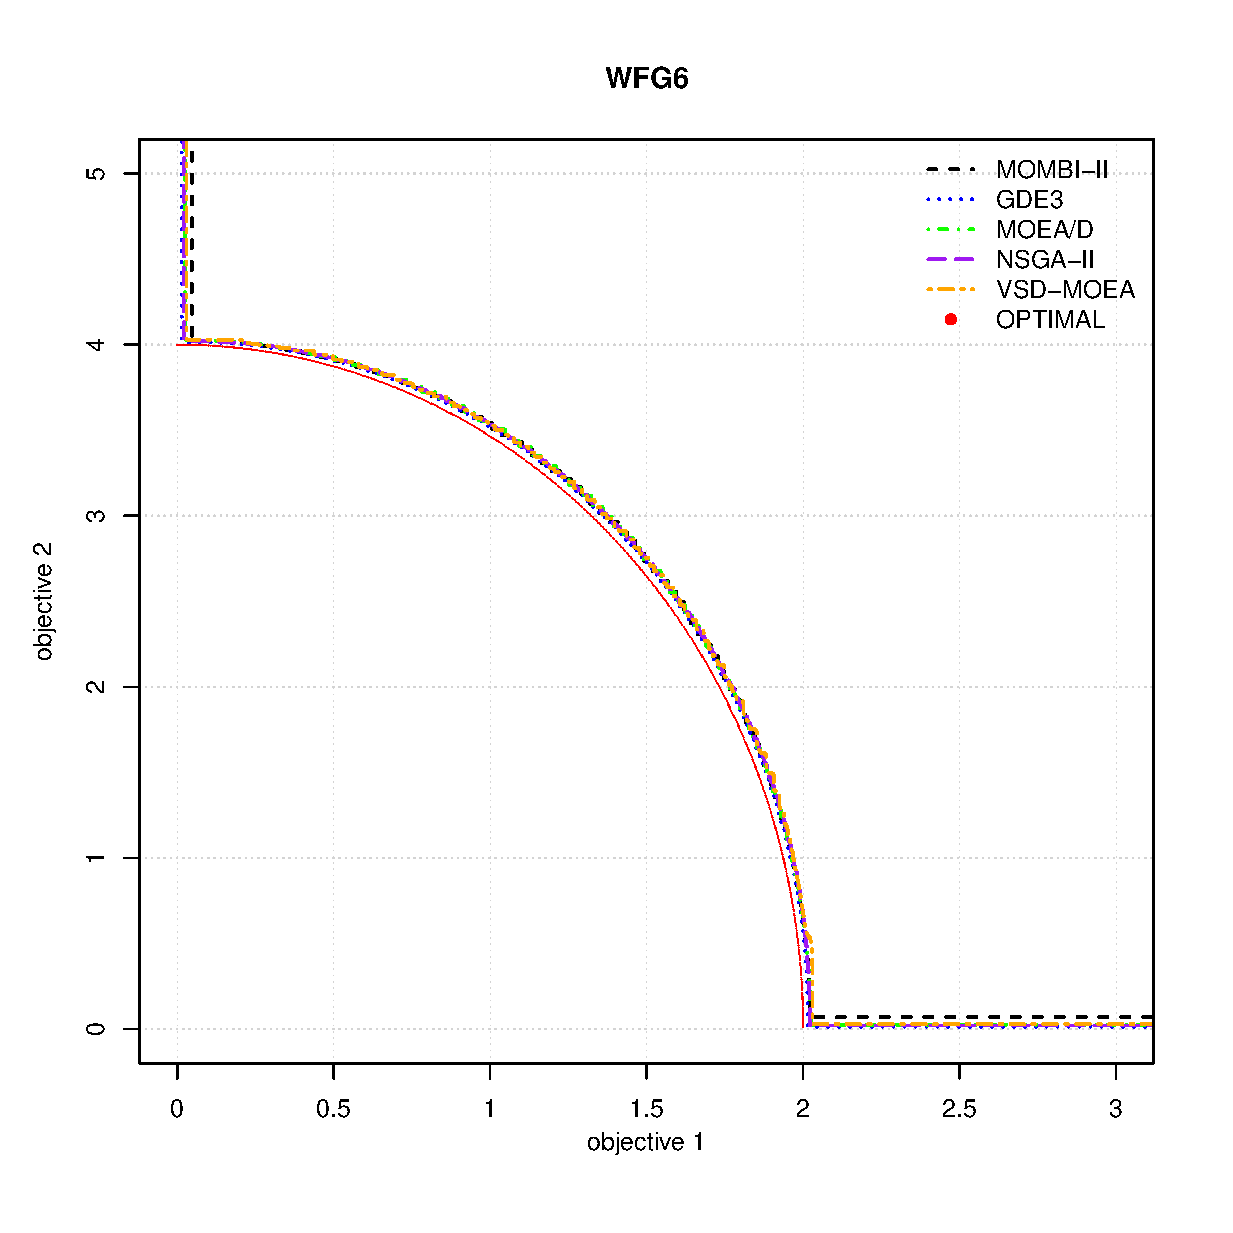
\includegraphics[width=0.33\textwidth]{Figures_Chapter7/Results_Chapter3/WFG6.eps} 
\\
  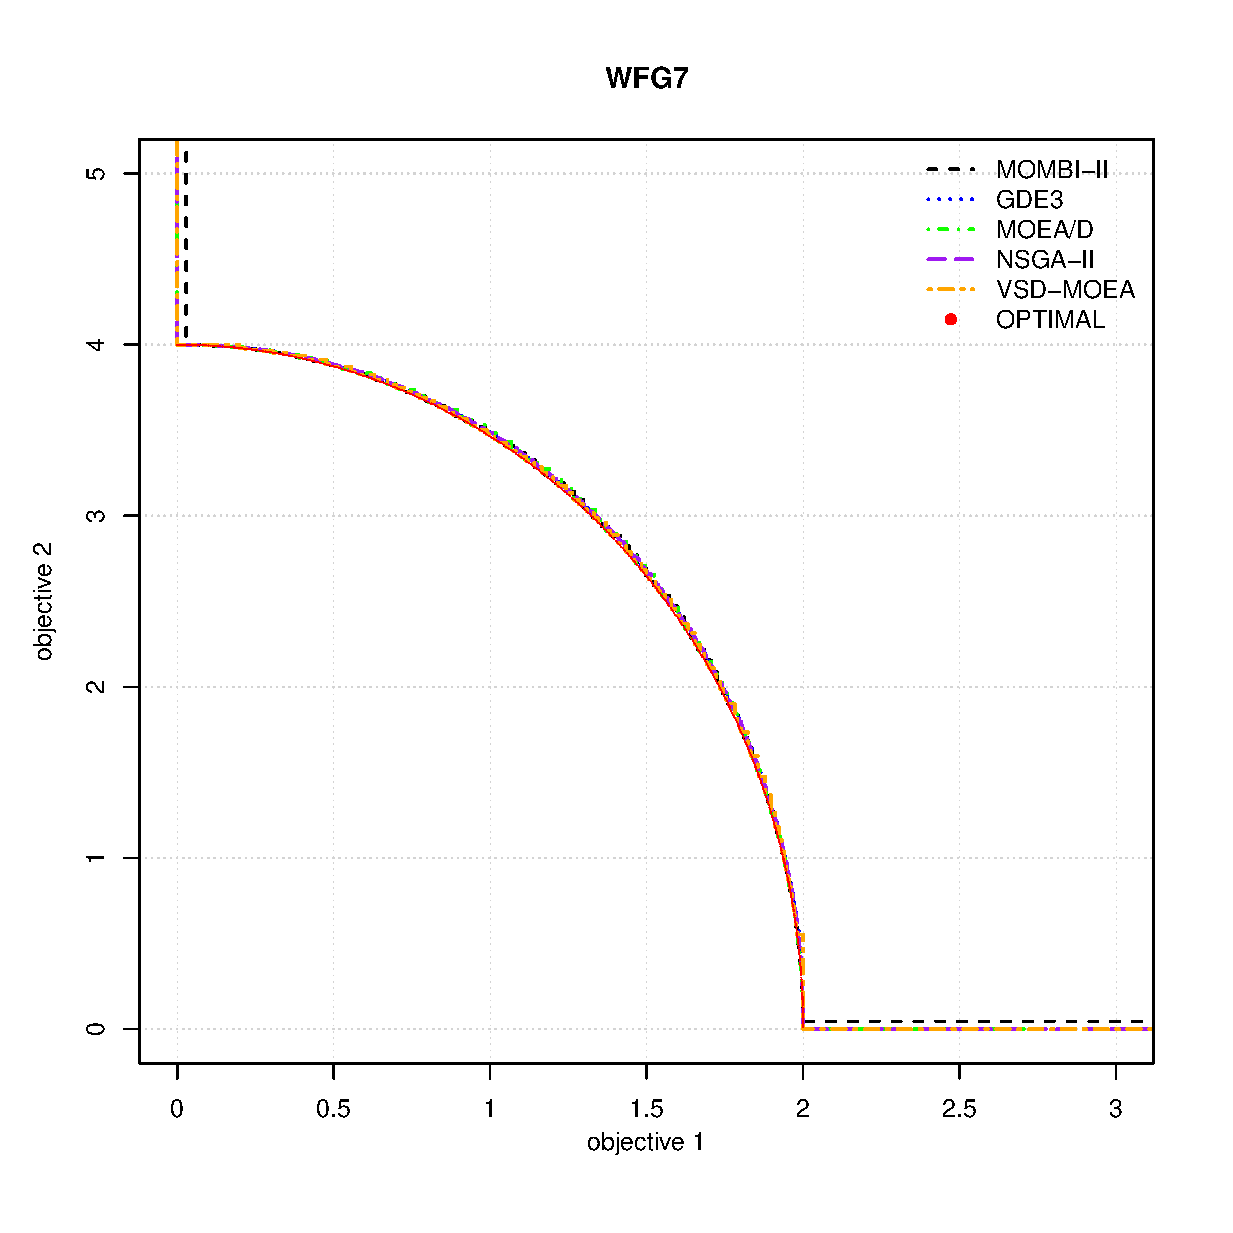
\includegraphics[width=0.33\textwidth]{Figures_Chapter7/Results_Chapter3/WFG7.eps} &
  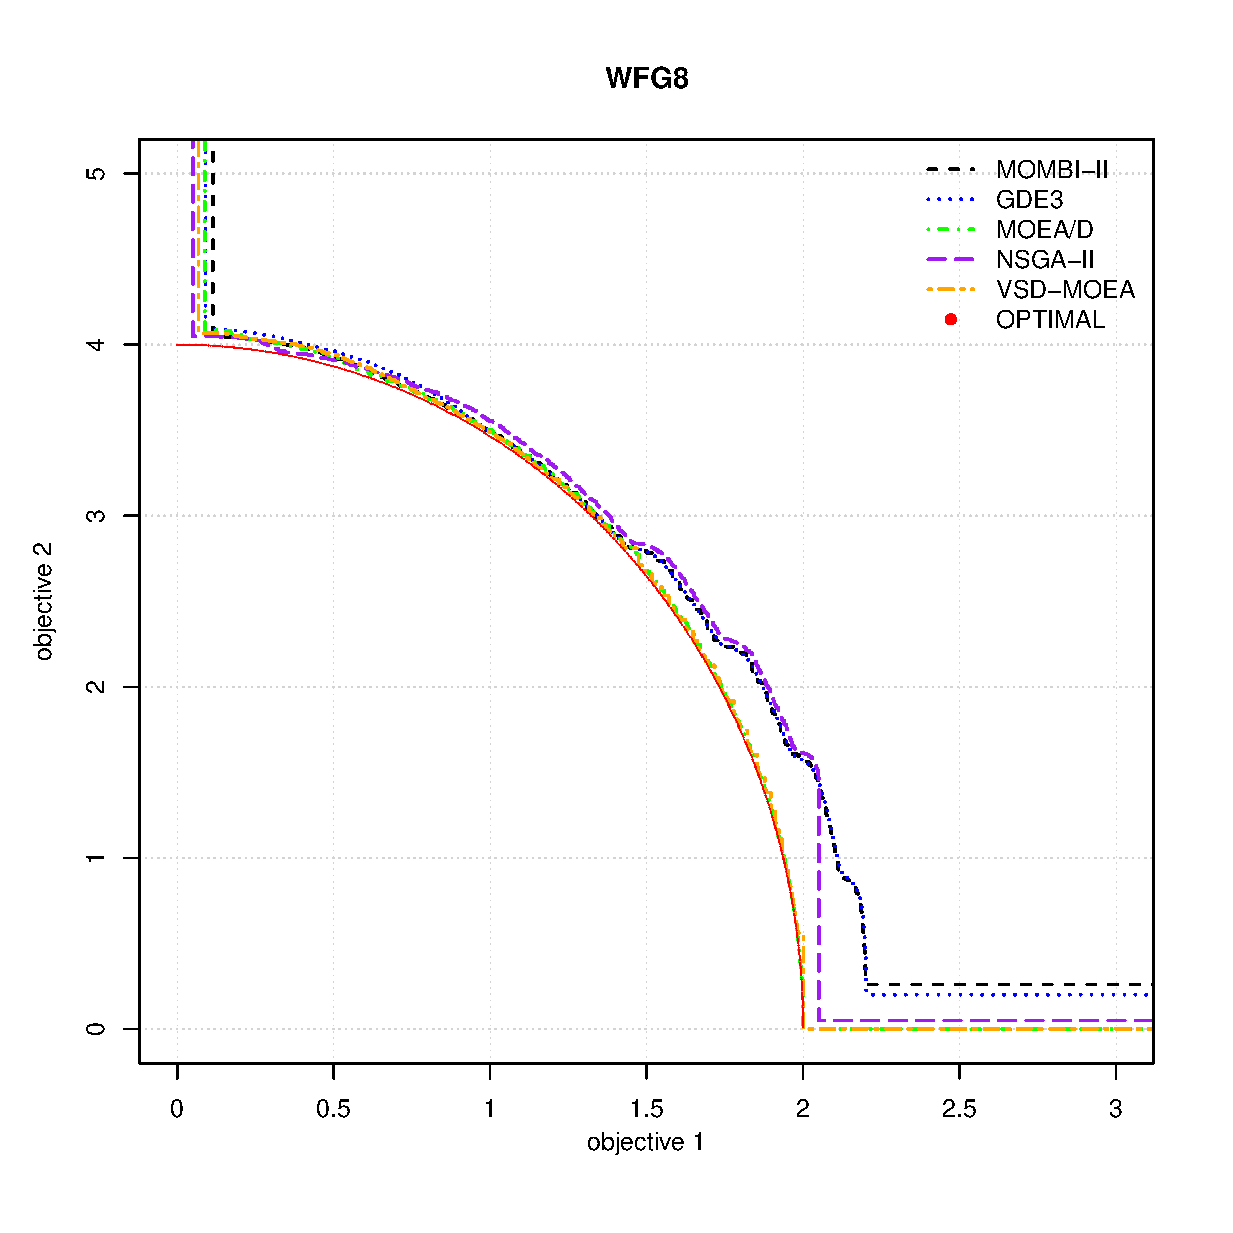
\includegraphics[width=0.33\textwidth]{Figures_Chapter7/Results_Chapter3/WFG8.eps} &
  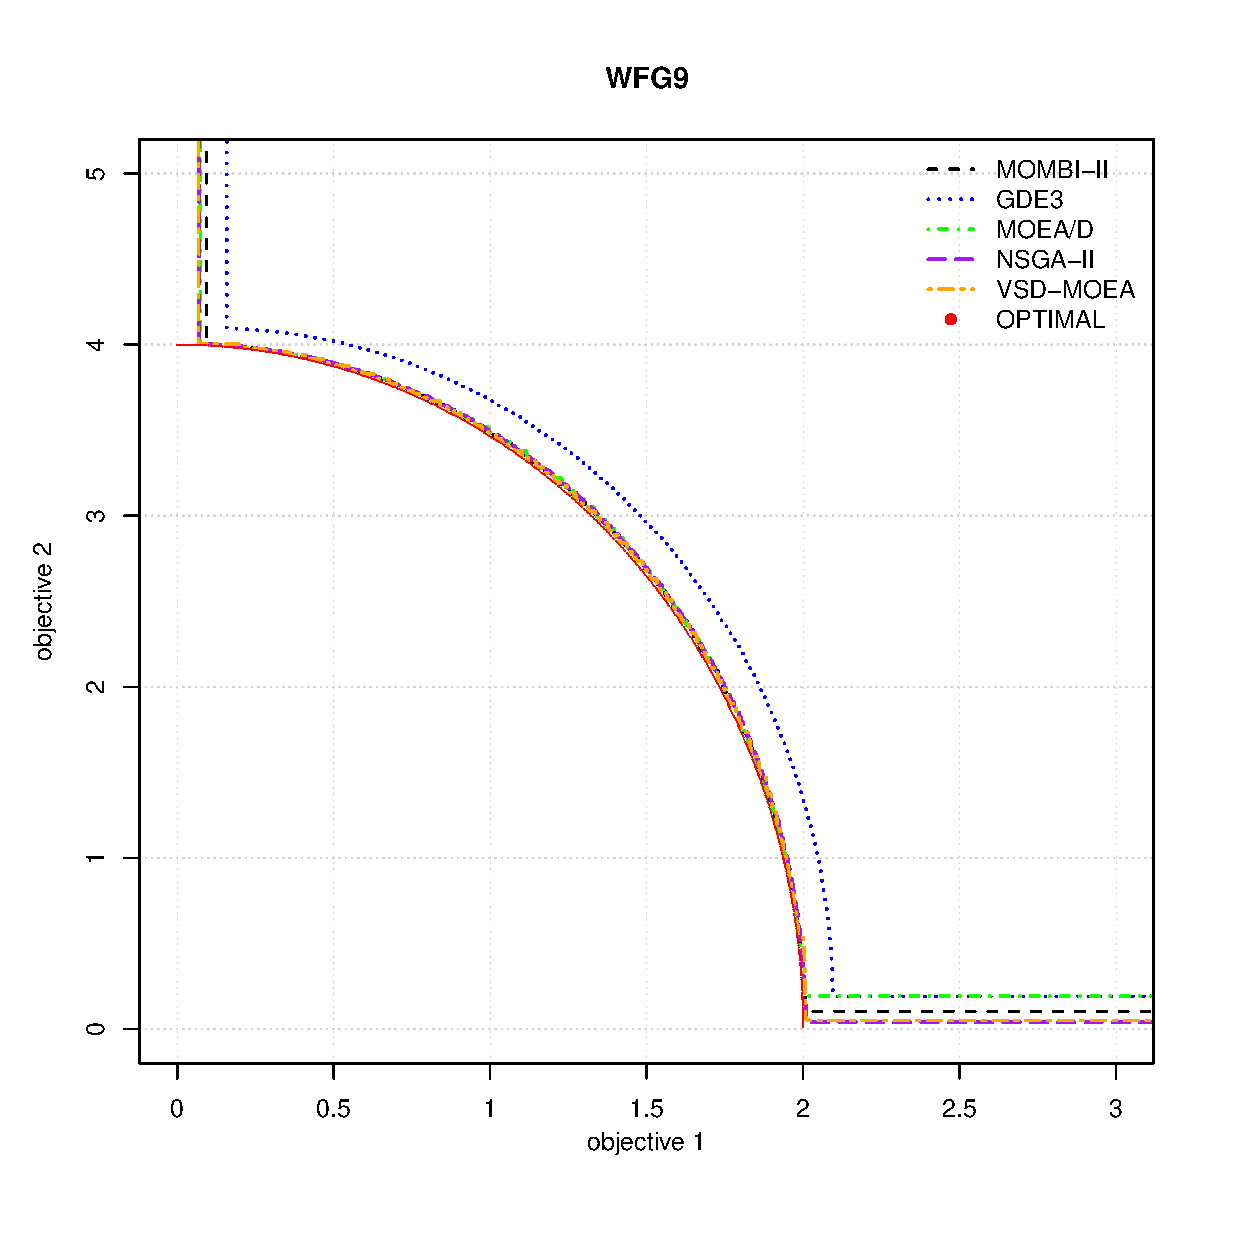
\includegraphics[width=0.33\textwidth]{Figures_Chapter7/Results_Chapter3/WFG9.eps}
\end{tabular}
\end{figure*}


%%\begin{figure}[h]
%%\centering
%%\caption{Estudio de escalabilidad en las variables de decisión considerando dos objetivos (Hipervolumen)}
%%\label{fig:Scalability_Study_HV_1}
%%\begin{tabular}{ccc}
%%   \includegraphics[width=0.2\textwidth, angle=-90,origin=c]{Figures_Chapter7/Results_Chapter3/DTLZ4_2obj_Scalability.eps} &
%%    \includegraphics[width=0.2\textwidth, angle=-90,origin=c]{Figures_Chapter7/Results_Chapter3/DTLZ7_2obj_Scalability.eps} &
%%    \includegraphics[width=0.2\textwidth,angle=-90,origin=c]{Figures_Chapter7/Results_Chapter3/UF7_Scalability.eps}  
%%    \\
%%       \includegraphics[width=0.2\textwidth, angle=-90,origin=c]{Figures_Chapter7/Results_Chapter3/UF5_Scalability.eps} &
%%    \includegraphics[width=0.2\textwidth, angle=-90,origin=c]{Figures_Chapter7/Results_Chapter3/WFG2_2obj_Scalability.eps} &
%%    \includegraphics[width=0.2\textwidth, angle=-90,origin=c]{Figures_Chapter7/Results_Chapter3/WFG8_2obj_Scalability.eps}  
%%
%%\end{tabular}
%%\end{figure}
%%
%%\begin{figure}[h]
%%\centering
%%\caption{Estudio de escalabilidad en las variables de decisión considerando tres objetivos (Hipervolumen)}
%%\label{fig:Scalability_Study_HV_1}
%%\begin{tabular}{ccc}
%%   \includegraphics[width=0.2\textwidth, angle=-90,origin=c]{Figures_Chapter7/Results_Chapter3/DTLZ4_3obj_Scalability.eps} &
%%    \includegraphics[width=0.2\textwidth, angle=-90,origin=c]{Figures_Chapter7/Results_Chapter3/DTLZ7_3obj_Scalability.eps} &
%%    \includegraphics[width=0.2\textwidth,  angle=-90,origin=c]{Figures_Chapter7/Results_Chapter3/UF10_Scalability.eps}  
%%    \\
%%    \includegraphics[width=0.2\textwidth, angle=-90,origin=c]{Figures_Chapter7/Results_Chapter3/WFG2_3obj_Scalability.eps} &
%%    \includegraphics[width=0.2\textwidth, angle=-90,origin=c]{Figures_Chapter7/Results_Chapter3/WFG8_3obj_Scalability.eps}  
%%\end{tabular}
%%\end{figure}
%%
%----------------------------------------------------------------------------------------

%
\begin{figure}[h]
\centering
\caption{Estudio del parámetro DI de la instancias DTLZ con dos objetivos}
\label{fig:Scalability_Study_HV_1}
\begin{tabular}{ccc}
   \includegraphics[width=0.2\textwidth, angle=-90,origin=c]{Figures_Chapter7/Results_Chapter3/EPS_DI/2obj_DTLZ1.eps} &
   \includegraphics[width=0.2\textwidth, angle=-90,origin=c]{Figures_Chapter7/Results_Chapter3/EPS_DI/2obj_DTLZ2.eps} &
   \includegraphics[width=0.2\textwidth,angle=-90,origin=c]{Figures_Chapter7/Results_Chapter3/EPS_DI/2obj_DTLZ3.eps}  
    \\ 
   \includegraphics[width=0.2\textwidth, angle=-90,origin=c]{Figures_Chapter7/Results_Chapter3/EPS_DI/2obj_DTLZ4.eps} &
   \includegraphics[width=0.2\textwidth, angle=-90,origin=c]{Figures_Chapter7/Results_Chapter3/EPS_DI/2obj_DTLZ5.eps} &
   \includegraphics[width=0.2\textwidth,angle=-90,origin=c]{Figures_Chapter7/Results_Chapter3/EPS_DI/2obj_DTLZ6.eps}
   \\
  \includegraphics[width=0.2\textwidth, angle=-90,origin=c]{Figures_Chapter7/Results_Chapter3/EPS_DI/2obj_DTLZ7.eps}
\end{tabular}
\end{figure}

\begin{figure}[h]
\centering
\caption{Estudio del parámetro DI de la instancias DTLZ con tres objetivos}
\label{fig:Scalability_Study_HV_1}
\begin{tabular}{ccc}
   \includegraphics[width=0.2\textwidth, angle=-90,origin=c]{Figures_Chapter7/Results_Chapter3/EPS_DI/3obj_DTLZ1.eps} &
   \includegraphics[width=0.2\textwidth, angle=-90,origin=c]{Figures_Chapter7/Results_Chapter3/EPS_DI/3obj_DTLZ2.eps} &
   \includegraphics[width=0.2\textwidth,angle=-90,origin=c]{Figures_Chapter7/Results_Chapter3/EPS_DI/3obj_DTLZ3.eps}  
    \\ 
   \includegraphics[width=0.2\textwidth, angle=-90,origin=c]{Figures_Chapter7/Results_Chapter3/EPS_DI/3obj_DTLZ4.eps} &
   \includegraphics[width=0.2\textwidth, angle=-90,origin=c]{Figures_Chapter7/Results_Chapter3/EPS_DI/3obj_DTLZ5.eps} &
   \includegraphics[width=0.2\textwidth,angle=-90,origin=c]{Figures_Chapter7/Results_Chapter3/EPS_DI/3obj_DTLZ6.eps}
   \\
  \includegraphics[width=0.2\textwidth, angle=-90,origin=c]{Figures_Chapter7/Results_Chapter3/EPS_DI/3obj_DTLZ7.eps}
\end{tabular}
\end{figure}


\begin{figure}[h]
\centering
\caption{Estudio del parámetro DI de la instancias WFG con dos objetivos}
\label{fig:Scalability_Study_HV_1}
\begin{tabular}{ccc}
   \includegraphics[width=0.2\textwidth, angle=-90,origin=c]{Figures_Chapter7/Results_Chapter3/EPS_DI/2obj_WFG1.eps} &
   \includegraphics[width=0.2\textwidth, angle=-90,origin=c]{Figures_Chapter7/Results_Chapter3/EPS_DI/2obj_WFG2.eps} &
   \includegraphics[width=0.2\textwidth,angle=-90,origin=c]{Figures_Chapter7/Results_Chapter3/EPS_DI/2obj_WFG3.eps}  
    \\ 
   \includegraphics[width=0.2\textwidth, angle=-90,origin=c]{Figures_Chapter7/Results_Chapter3/EPS_DI/2obj_WFG4.eps} &
   \includegraphics[width=0.2\textwidth, angle=-90,origin=c]{Figures_Chapter7/Results_Chapter3/EPS_DI/2obj_WFG5.eps} &
   \includegraphics[width=0.2\textwidth,angle=-90,origin=c]{Figures_Chapter7/Results_Chapter3/EPS_DI/2obj_WFG6.eps}
   \\
  \includegraphics[width=0.2\textwidth, angle=-90,origin=c]{Figures_Chapter7/Results_Chapter3/EPS_DI/2obj_WFG7.eps} &
   \includegraphics[width=0.2\textwidth, angle=-90,origin=c]{Figures_Chapter7/Results_Chapter3/EPS_DI/2obj_WFG8.eps} &
   \includegraphics[width=0.2\textwidth,angle=-90,origin=c]{Figures_Chapter7/Results_Chapter3/EPS_DI/2obj_WFG9.eps}
\end{tabular}
\end{figure}

\begin{figure*}[h]
\centering
\caption{Estudio del parámetro DI de la instancias WFG con tres objetivos}
\label{fig:Scalability_Study_HV_1}
\begin{tabular}{ccc}
   \includegraphics[width=0.2\textwidth, angle=-90,origin=c]{Figures_Chapter7/Results_Chapter3/EPS_DI/3obj_WFG1.eps} &
   \includegraphics[width=0.2\textwidth, angle=-90,origin=c]{Figures_Chapter7/Results_Chapter3/EPS_DI/3obj_WFG2.eps} &
   \includegraphics[width=0.2\textwidth,angle=-90,origin=c]{Figures_Chapter7/Results_Chapter3/EPS_DI/3obj_WFG3.eps}  
    \\ 
   \includegraphics[width=0.2\textwidth, angle=-90,origin=c]{Figures_Chapter7/Results_Chapter3/EPS_DI/3obj_WFG4.eps} &
   \includegraphics[width=0.2\textwidth, angle=-90,origin=c]{Figures_Chapter7/Results_Chapter3/EPS_DI/3obj_WFG5.eps} &
   \includegraphics[width=0.2\textwidth,angle=-90,origin=c]{Figures_Chapter7/Results_Chapter3/EPS_DI/3obj_WFG6.eps}
   \\
  \includegraphics[width=0.2\textwidth, angle=-90,origin=c]{Figures_Chapter7/Results_Chapter3/EPS_DI/3obj_WFG7.eps} &
   \includegraphics[width=0.2\textwidth, angle=-90,origin=c]{Figures_Chapter7/Results_Chapter3/EPS_DI/3obj_WFG8.eps} &
   \includegraphics[width=0.2\textwidth,angle=-90,origin=c]{Figures_Chapter7/Results_Chapter3/EPS_DI/3obj_WFG9.eps}
\end{tabular}
\end{figure*}


\begin{figure*}[h]
\centering
\caption{Estudio del parámetro DI de la instancias UF con dos y tres objetivos}
\label{fig:Scalability_Study_HV_1}
\begin{tabular}{ccc}
   \includegraphics[width=0.2\textwidth, angle=-90,origin=c]{Figures_Chapter7/Results_Chapter3/EPS_DI/UF1.eps} &
   \includegraphics[width=0.2\textwidth, angle=-90,origin=c]{Figures_Chapter7/Results_Chapter3/EPS_DI/UF2.eps} &
   \includegraphics[width=0.2\textwidth,angle=-90,origin=c]{Figures_Chapter7/Results_Chapter3/EPS_DI/UF3.eps}  
    \\ 
   \includegraphics[width=0.2\textwidth, angle=-90,origin=c]{Figures_Chapter7/Results_Chapter3/EPS_DI/UF4.eps} &
   \includegraphics[width=0.2\textwidth, angle=-90,origin=c]{Figures_Chapter7/Results_Chapter3/EPS_DI/UF5.eps} &
   \includegraphics[width=0.2\textwidth,angle=-90,origin=c]{Figures_Chapter7/Results_Chapter3/EPS_DI/UF6.eps}
   \\
  \includegraphics[width=0.2\textwidth, angle=-90,origin=c]{Figures_Chapter7/Results_Chapter3/EPS_DI/UF7.eps} &
   \includegraphics[width=0.2\textwidth, angle=-90,origin=c]{Figures_Chapter7/Results_Chapter3/EPS_DI/UF8.eps} &
   \includegraphics[width=0.2\textwidth,angle=-90,origin=c]{Figures_Chapter7/Results_Chapter3/EPS_DI/UF9.eps}
   \\
   \includegraphics[width=0.2\textwidth,angle=-90,origin=c]{Figures_Chapter7/Results_Chapter3/EPS_DI/UF10.eps}
\end{tabular}
\end{figure*}

